% The IEEE short version of the thesis (thesis_revised/). Every number is the thesis's own \V{key},
% read from generated/numbers.tex, and the tables and figures come from make_ieee_assets.py, which
% copies them from the thesis with each design named in words. Build with Tectonic:
%   python IEEE_Conference_Template/make_ieee_assets.py   (from src/probes/deception-detection)
%   tectonic main.tex --keep-logs                          (in this folder)
\documentclass[conference]{IEEEtran}
\usepackage{cite}
\usepackage{amsmath,amssymb,amsfonts}
% IEEEtran asks for Times, which XeTeX (Tectonic) has only as the OpenType clone TeX Gyre Termes,
% found by file name because Tectonic has no font configuration.
\usepackage{fontspec}
\setmainfont{texgyretermes}[Extension=.otf, UprightFont=*-regular, BoldFont=*-bold,
  ItalicFont=*-italic, BoldItalicFont=*-bolditalic]
\usepackage{graphicx}
\usepackage{textcomp}
\usepackage{xcolor}
\usepackage{booktabs,multirow,tabularx}
\usepackage{tikz} % the knowledge direction's diagram
\usetikzlibrary{arrows.meta,positioning,calc}
\usepackage[hidelinks]{hyperref}
\usepackage[capitalize]{cleveref} % must follow hyperref
\crefname{figure}{Fig.}{Figs.}
\Crefname{figure}{Fig.}{Figs.}
\crefname{table}{Table}{Tables}
\crefname{section}{Section}{Sections}
\crefformat{equation}{(#2#1#3)}
\crefmultiformat{equation}{(#2#1#3)}{ and~(#2#1#3)}{, (#2#1#3)}{ and~(#2#1#3)}
\graphicspath{{images/}}

% Every result is the thesis's, read as \V{key}; an unknown key stops the build instead of printing
% a blank.
\makeatletter
\newcommand{\setV}[2]{\expandafter\def\csname num@#1\endcsname{#2}}
\newcommand{\V}[1]{\ifcsname num@#1\endcsname\csname num@#1\endcsname\else
  \PackageError{numbers}{Undefined number `#1'}{Run make_ieee_assets.py}\fi}
\makeatother
% Generated by make_numbers.py -- do not edit.
\setV{n-cg}{267}
\setV{ndec-cg}{167}
\setV{n-hpc}{2,134}
\setV{ndec-hpc}{134}
\setV{n-hpkr}{2,139}
\setV{ndec-hpkr}{139}
\setV{n-it}{1,080}
\setV{ndec-it}{423}
\setV{n-id}{5,432}
\setV{ndec-id}{3,045}
\setV{n-repe}{550}
\setV{ndec-repe}{275}
\setV{n-control}{2,000}
\setV{bank-personas}{36}
\setV{bank-new}{10}
\setV{bank-kept}{3,749}
\setV{bank-generated}{5,400}
\setV{bank-kept-min}{47}
\setV{bank-kept-max}{149}
\setV{bank-kept-pct}{69}
\setV{zs-dec-cg-L20}{0.940}
\setV{zs-dec-hpc-L20}{0.717}
\setV{zs-dec-hpkr-L20}{0.148}
\setV{zs-dec-it-L20}{0.988}
\setV{zs-dec-id-L20}{0.959}
\setV{zs-dec-repe-L20}{0.994}
\setV{zs-dec-mean-L20}{0.791}
\setV{zs-dec-lb-L20}{0.750}
\setV{zs-den-cg-L20}{0.931}
\setV{zs-den-hpc-L20}{0.585}
\setV{zs-den-hpkr-L20}{0.890}
\setV{zs-den-it-L20}{0.976}
\setV{zs-den-id-L20}{0.932}
\setV{zs-den-repe-L20}{0.882}
\setV{zs-den-mean-L20}{0.866}
\setV{zs-den-lb-L20}{0.863}
\setV{zs-ext-cg-L20}{0.969}
\setV{zs-ext-hpc-L20}{0.639}
\setV{zs-ext-hpkr-L20}{0.882}
\setV{zs-ext-it-L20}{0.990}
\setV{zs-ext-id-L20}{0.954}
\setV{zs-ext-repe-L20}{0.991}
\setV{zs-ext-mean-L20}{0.904}
\setV{zs-ext-lb-L20}{0.887}
\setV{zs-syc-cg-L20}{0.999}
\setV{zs-syc-hpc-L20}{0.533}
\setV{zs-syc-hpkr-L20}{0.043}
\setV{zs-syc-it-L20}{0.983}
\setV{zs-syc-id-L20}{0.923}
\setV{zs-syc-repe-L20}{0.977}
\setV{zs-syc-mean-L20}{0.743}
\setV{zs-syc-lb-L20}{0.696}
\setV{zs-pcone-cg-L20}{0.942}
\setV{zs-pcone-hpc-L20}{0.700}
\setV{zs-pcone-hpkr-L20}{0.253}
\setV{zs-pcone-it-L20}{0.989}
\setV{zs-pcone-id-L20}{0.959}
\setV{zs-pcone-repe-L20}{0.991}
\setV{zs-pcone-mean-L20}{0.806}
\setV{zs-pcone-lb-L20}{0.769}
\setV{zs-extpcone-cg-L20}{0.737}
\setV{zs-extpcone-hpc-L20}{0.615}
\setV{zs-extpcone-hpkr-L20}{0.559}
\setV{zs-extpcone-it-L20}{0.681}
\setV{zs-extpcone-id-L20}{0.772}
\setV{zs-extpcone-repe-L20}{0.604}
\setV{zs-extpcone-mean-L20}{0.661}
\setV{zs-extpcone-lb-L20}{0.673}
\setV{zs-dec-cg-L40}{0.865}
\setV{zs-dec-hpc-L40}{0.581}
\setV{zs-dec-hpkr-L40}{0.593}
\setV{zs-dec-it-L40}{0.979}
\setV{zs-dec-id-L40}{0.974}
\setV{zs-dec-repe-L40}{1.000}
\setV{zs-dec-mean-L40}{0.832}
\setV{zs-dec-lb-L40}{0.798}
\setV{zs-den-cg-L40}{0.902}
\setV{zs-den-hpc-L40}{0.755}
\setV{zs-den-hpkr-L40}{0.919}
\setV{zs-den-it-L40}{0.913}
\setV{zs-den-id-L40}{0.980}
\setV{zs-den-repe-L40}{1.000}
\setV{zs-den-mean-L40}{0.912}
\setV{zs-den-lb-L40}{0.894}
\setV{zs-ext-cg-L40}{0.912}
\setV{zs-ext-hpc-L40}{0.712}
\setV{zs-ext-hpkr-L40}{0.912}
\setV{zs-ext-it-L40}{0.980}
\setV{zs-ext-id-L40}{0.978}
\setV{zs-ext-repe-L40}{1.000}
\setV{zs-ext-mean-L40}{0.916}
\setV{zs-ext-lb-L40}{0.899}
\setV{zs-syc-cg-L40}{0.998}
\setV{zs-syc-hpc-L40}{0.751}
\setV{zs-syc-hpkr-L40}{0.167}
\setV{zs-syc-it-L40}{0.985}
\setV{zs-syc-id-L40}{0.948}
\setV{zs-syc-repe-L40}{0.999}
\setV{zs-syc-mean-L40}{0.808}
\setV{zs-syc-lb-L40}{0.770}
\setV{zs-pcone-cg-L40}{0.906}
\setV{zs-pcone-hpc-L40}{0.599}
\setV{zs-pcone-hpkr-L40}{0.693}
\setV{zs-pcone-it-L40}{0.982}
\setV{zs-pcone-id-L40}{0.975}
\setV{zs-pcone-repe-L40}{1.000}
\setV{zs-pcone-mean-L40}{0.859}
\setV{zs-pcone-lb-L40}{0.831}
\setV{zs-extpcone-cg-L40}{0.813}
\setV{zs-extpcone-hpc-L40}{0.564}
\setV{zs-extpcone-hpkr-L40}{0.736}
\setV{zs-extpcone-it-L40}{0.546}
\setV{zs-extpcone-id-L40}{0.958}
\setV{zs-extpcone-repe-L40}{0.990}
\setV{zs-extpcone-mean-L40}{0.768}
\setV{zs-extpcone-lb-L40}{0.723}
\setV{zs-dec-cg-L44}{0.819}
\setV{zs-dec-hpc-L44}{0.607}
\setV{zs-dec-hpkr-L44}{0.589}
\setV{zs-dec-it-L44}{0.979}
\setV{zs-dec-id-L44}{0.962}
\setV{zs-dec-repe-L44}{1.000}
\setV{zs-dec-mean-L44}{0.826}
\setV{zs-dec-lb-L44}{0.791}
\setV{zs-den-cg-L44}{0.858}
\setV{zs-den-hpc-L44}{0.725}
\setV{zs-den-hpkr-L44}{0.908}
\setV{zs-den-it-L44}{0.933}
\setV{zs-den-id-L44}{0.978}
\setV{zs-den-repe-L44}{1.000}
\setV{zs-den-mean-L44}{0.900}
\setV{zs-den-lb-L44}{0.880}
\setV{zs-ext-cg-L44}{0.859}
\setV{zs-ext-hpc-L44}{0.712}
\setV{zs-ext-hpkr-L44}{0.894}
\setV{zs-ext-it-L44}{0.982}
\setV{zs-ext-id-L44}{0.974}
\setV{zs-ext-repe-L44}{1.000}
\setV{zs-ext-mean-L44}{0.903}
\setV{zs-ext-lb-L44}{0.884}
\setV{zs-syc-cg-L44}{0.983}
\setV{zs-syc-hpc-L44}{0.692}
\setV{zs-syc-hpkr-L44}{0.480}
\setV{zs-syc-it-L44}{0.987}
\setV{zs-syc-id-L44}{0.949}
\setV{zs-syc-repe-L44}{1.000}
\setV{zs-syc-mean-L44}{0.848}
\setV{zs-syc-lb-L44}{0.818}
\setV{zs-pcone-cg-L44}{0.859}
\setV{zs-pcone-hpc-L44}{0.633}
\setV{zs-pcone-hpkr-L44}{0.665}
\setV{zs-pcone-it-L44}{0.982}
\setV{zs-pcone-id-L44}{0.966}
\setV{zs-pcone-repe-L44}{1.000}
\setV{zs-pcone-mean-L44}{0.851}
\setV{zs-pcone-lb-L44}{0.821}
\setV{zs-extpcone-cg-L44}{0.784}
\setV{zs-extpcone-hpc-L44}{0.583}
\setV{zs-extpcone-hpkr-L44}{0.715}
\setV{zs-extpcone-it-L44}{0.663}
\setV{zs-extpcone-id-L44}{0.962}
\setV{zs-extpcone-repe-L44}{0.973}
\setV{zs-extpcone-mean-L44}{0.780}
\setV{zs-extpcone-lb-L44}{0.742}
\setV{off-base-L20}{0.648}
\setV{offx-base-L20}{0.728}
\setV{diag-base-L20}{0.956}
\setV{off-dec-L20}{0.651}
\setV{offx-dec-L20}{0.919}
\setV{diag-dec-L20}{0.908}
\setV{off-den-L20}{0.866}
\setV{offx-den-L20}{0.861}
\setV{diag-den-L20}{0.865}
\setV{off-ext-L20}{0.904}
\setV{offx-ext-L20}{0.909}
\setV{diag-ext-L20}{0.904}
\setV{off-pcone-L20}{0.667}
\setV{offx-pcone-L20}{0.916}
\setV{diag-pcone-L20}{0.887}
\setV{off-pcthree-L20}{0.679}
\setV{offx-pcthree-L20}{0.888}
\setV{diag-pcthree-L20}{0.919}
\setV{off-extpcone-L20}{0.661}
\setV{offx-extpcone-L20}{0.682}
\setV{diag-extpcone-L20}{0.643}
\setV{off-extpcthree-L20}{0.684}
\setV{offx-extpcthree-L20}{0.900}
\setV{diag-extpcthree-L20}{0.915}
\setV{off-denpcthree-L20}{0.710}
\setV{offx-denpcthree-L20}{0.752}
\setV{diag-denpcthree-L20}{0.875}
\setV{off-rand-L20}{0.527}
\setV{offx-rand-L20}{0.560}
\setV{diag-rand-L20}{0.787}
\setV{off-syc-L20}{0.615}
\setV{offx-syc-L20}{0.883}
\setV{diag-syc-L20}{0.892}
\setV{off-sycpcone-L20}{0.615}
\setV{offx-sycpcone-L20}{0.884}
\setV{diag-sycpcone-L20}{0.893}
\setV{off-sycthree-L20}{0.657}
\setV{offx-sycthree-L20}{0.823}
\setV{diag-sycthree-L20}{0.931}
\setV{gap-ext-base-L20}{0.256}
\setV{gap-ext-extpcthree-L20}{0.220}
\setV{gap-ext-dec-L20}{0.253}
\setV{drop-base-L20}{0.309}
\setV{pt-base-cg-L20}{0.663}
\setV{pt-base-hpc-L20}{0.535}
\setV{pt-base-hpkr-L20}{0.394}
\setV{pt-base-it-L20}{0.799}
\setV{pt-base-id-L20}{0.778}
\setV{pt-base-repe-L20}{0.718}
\setV{pt-dec-cg-L20}{0.764}
\setV{pt-dec-hpc-L20}{0.630}
\setV{pt-dec-hpkr-L20}{0.148}
\setV{pt-dec-it-L20}{0.793}
\setV{pt-dec-id-L20}{0.775}
\setV{pt-dec-repe-L20}{0.796}
\setV{pt-den-cg-L20}{0.931}
\setV{pt-den-hpc-L20}{0.585}
\setV{pt-den-hpkr-L20}{0.890}
\setV{pt-den-it-L20}{0.976}
\setV{pt-den-id-L20}{0.932}
\setV{pt-den-repe-L20}{0.883}
\setV{pt-ext-cg-L20}{0.969}
\setV{pt-ext-hpc-L20}{0.639}
\setV{pt-ext-hpkr-L20}{0.882}
\setV{pt-ext-it-L20}{0.990}
\setV{pt-ext-id-L20}{0.954}
\setV{pt-ext-repe-L20}{0.991}
\setV{off-base-L40}{0.732}
\setV{offx-base-L40}{0.758}
\setV{diag-base-L40}{0.983}
\setV{off-dec-L40}{0.832}
\setV{offx-dec-L40}{0.880}
\setV{diag-dec-L40}{0.829}
\setV{off-den-L40}{0.912}
\setV{offx-den-L40}{0.910}
\setV{diag-den-L40}{0.911}
\setV{off-ext-L40}{0.916}
\setV{offx-ext-L40}{0.917}
\setV{diag-ext-L40}{0.916}
\setV{off-pcone-L40}{0.859}
\setV{offx-pcone-L40}{0.893}
\setV{diag-pcone-L40}{0.858}
\setV{off-pcthree-L40}{0.639}
\setV{offx-pcthree-L40}{0.751}
\setV{diag-pcthree-L40}{0.916}
\setV{off-extpcone-L40}{0.768}
\setV{offx-extpcone-L40}{0.774}
\setV{diag-extpcone-L40}{0.764}
\setV{off-extpcthree-L40}{0.866}
\setV{offx-extpcthree-L40}{0.867}
\setV{diag-extpcthree-L40}{0.943}
\setV{off-denpcthree-L40}{0.872}
\setV{offx-denpcthree-L40}{0.873}
\setV{diag-denpcthree-L40}{0.926}
\setV{off-rand-L40}{0.504}
\setV{offx-rand-L40}{0.544}
\setV{diag-rand-L40}{0.807}
\setV{off-syc-L40}{0.663}
\setV{offx-syc-L40}{0.936}
\setV{diag-syc-L40}{0.919}
\setV{off-sycpcone-L40}{0.662}
\setV{offx-sycpcone-L40}{0.937}
\setV{diag-sycpcone-L40}{0.920}
\setV{off-sycthree-L40}{0.697}
\setV{offx-sycthree-L40}{0.888}
\setV{diag-sycthree-L40}{0.937}
\setV{gap-ext-base-L40}{0.184}
\setV{gap-ext-extpcthree-L40}{0.050}
\setV{gap-ext-dec-L40}{0.084}
\setV{drop-base-L40}{0.251}
\setV{pt-base-cg-L40}{0.787}
\setV{pt-base-hpc-L40}{0.571}
\setV{pt-base-hpkr-L40}{0.584}
\setV{pt-base-it-L40}{0.800}
\setV{pt-base-id-L40}{0.827}
\setV{pt-base-repe-L40}{0.824}
\setV{pt-dec-cg-L40}{0.865}
\setV{pt-dec-hpc-L40}{0.581}
\setV{pt-dec-hpkr-L40}{0.593}
\setV{pt-dec-it-L40}{0.979}
\setV{pt-dec-id-L40}{0.974}
\setV{pt-dec-repe-L40}{1.000}
\setV{pt-den-cg-L40}{0.902}
\setV{pt-den-hpc-L40}{0.755}
\setV{pt-den-hpkr-L40}{0.919}
\setV{pt-den-it-L40}{0.913}
\setV{pt-den-id-L40}{0.980}
\setV{pt-den-repe-L40}{1.000}
\setV{pt-ext-cg-L40}{0.912}
\setV{pt-ext-hpc-L40}{0.712}
\setV{pt-ext-hpkr-L40}{0.912}
\setV{pt-ext-it-L40}{0.980}
\setV{pt-ext-id-L40}{0.978}
\setV{pt-ext-repe-L40}{1.000}
\setV{off-base-L44}{0.716}
\setV{offx-base-L44}{0.730}
\setV{diag-base-L44}{0.982}
\setV{off-dec-L44}{0.826}
\setV{offx-dec-L44}{0.873}
\setV{diag-dec-L44}{0.821}
\setV{off-den-L44}{0.900}
\setV{offx-den-L44}{0.899}
\setV{diag-den-L44}{0.900}
\setV{off-ext-L44}{0.903}
\setV{offx-ext-L44}{0.905}
\setV{diag-ext-L44}{0.903}
\setV{off-pcone-L44}{0.851}
\setV{offx-pcone-L44}{0.888}
\setV{diag-pcone-L44}{0.849}
\setV{off-pcthree-L44}{0.617}
\setV{offx-pcthree-L44}{0.728}
\setV{diag-pcthree-L44}{0.916}
\setV{off-extpcone-L44}{0.780}
\setV{offx-extpcone-L44}{0.793}
\setV{diag-extpcone-L44}{0.778}
\setV{off-extpcthree-L44}{0.880}
\setV{offx-extpcthree-L44}{0.870}
\setV{diag-extpcthree-L44}{0.931}
\setV{off-denpcthree-L44}{0.870}
\setV{offx-denpcthree-L44}{0.864}
\setV{diag-denpcthree-L44}{0.915}
\setV{off-rand-L44}{0.493}
\setV{offx-rand-L44}{0.547}
\setV{diag-rand-L44}{0.796}
\setV{off-syc-L44}{0.708}
\setV{offx-syc-L44}{0.922}
\setV{diag-syc-L44}{0.852}
\setV{off-sycpcone-L44}{0.859}
\setV{offx-sycpcone-L44}{0.927}
\setV{diag-sycpcone-L44}{0.845}
\setV{off-sycthree-L44}{0.813}
\setV{offx-sycthree-L44}{0.882}
\setV{diag-sycthree-L44}{0.931}
\setV{gap-ext-base-L44}{0.188}
\setV{gap-ext-extpcthree-L44}{0.023}
\setV{gap-ext-dec-L44}{0.077}
\setV{drop-base-L44}{0.267}
\setV{pt-base-cg-L44}{0.757}
\setV{pt-base-hpc-L44}{0.570}
\setV{pt-base-hpkr-L44}{0.637}
\setV{pt-base-it-L44}{0.736}
\setV{pt-base-id-L44}{0.808}
\setV{pt-base-repe-L44}{0.785}
\setV{pt-dec-cg-L44}{0.819}
\setV{pt-dec-hpc-L44}{0.607}
\setV{pt-dec-hpkr-L44}{0.590}
\setV{pt-dec-it-L44}{0.979}
\setV{pt-dec-id-L44}{0.962}
\setV{pt-dec-repe-L44}{1.000}
\setV{pt-den-cg-L44}{0.858}
\setV{pt-den-hpc-L44}{0.725}
\setV{pt-den-hpkr-L44}{0.908}
\setV{pt-den-it-L44}{0.932}
\setV{pt-den-id-L44}{0.978}
\setV{pt-den-repe-L44}{1.000}
\setV{pt-ext-cg-L44}{0.859}
\setV{pt-ext-hpc-L44}{0.712}
\setV{pt-ext-hpkr-L44}{0.894}
\setV{pt-ext-it-L44}{0.982}
\setV{pt-ext-id-L44}{0.974}
\setV{pt-ext-repe-L44}{1.000}
\setV{balacc-off-base-L20}{0.554}
\setV{floor-base-L20}{15}
\setV{balacc-off-ext-L20}{0.651}
\setV{floor-ext-L20}{10}
\setV{balacc-off-den-L20}{0.594}
\setV{floor-den-L20}{10}
\setV{floor-cells-L20}{30}
\setV{balacc-off-base-L40}{0.592}
\setV{floor-base-L40}{18}
\setV{balacc-off-ext-L40}{0.745}
\setV{floor-ext-L40}{10}
\setV{balacc-off-den-L40}{0.771}
\setV{floor-den-L40}{5}
\setV{floor-cells-L40}{30}
\setV{balacc-off-base-L44}{0.592}
\setV{floor-base-L44}{17}
\setV{balacc-off-ext-L44}{0.722}
\setV{floor-ext-L44}{10}
\setV{balacc-off-den-L44}{0.734}
\setV{floor-den-L44}{10}
\setV{floor-cells-L44}{30}
\setV{op-base-balacc-L20}{0.721}
\setV{op-base-balacc-lo-L20}{0.713}
\setV{op-base-balacc-hi-L20}{0.728}
\setV{op-base-balacc-cg-L20}{0.838}
\setV{op-base-balacc-hpc-L20}{0.500}
\setV{op-base-balacc-hpkr-L20}{0.500}
\setV{op-base-balacc-it-L20}{0.909}
\setV{op-base-balacc-id-L20}{0.858}
\setV{op-base-balacc-repe-L20}{1.000}
\setV{op-base-recall-L20}{0.489}
\setV{op-base-recall-lo-L20}{0.475}
\setV{op-base-recall-hi-L20}{0.503}
\setV{op-base-recall-cg-L20}{0.677}
\setV{op-base-recall-hpc-L20}{0.000}
\setV{op-base-recall-hpkr-L20}{0.000}
\setV{op-base-recall-it-L20}{0.948}
\setV{op-base-recall-id-L20}{0.822}
\setV{op-base-recall-repe-L20}{1.000}
\setV{op-base-auroc-L20}{0.697}
\setV{op-base-auroc-lo-L20}{0.685}
\setV{op-base-auroc-hi-L20}{0.709}
\setV{op-base-auroc-cg-L20}{0.984}
\setV{op-base-auroc-hpc-L20}{0.471}
\setV{op-base-auroc-hpkr-L20}{0.109}
\setV{op-base-auroc-it-L20}{0.973}
\setV{op-base-auroc-id-L20}{0.950}
\setV{op-base-auroc-repe-L20}{1.000}
\setV{fp-base-cg-L20}{0}
\setV{fp-base-hpc-L20}{0}
\setV{fp-base-hpkr-L20}{0}
\setV{fp-base-it-L20}{13}
\setV{fp-base-id-L20}{11}
\setV{fp-base-repe-L20}{0}
\setV{op-dec-balacc-L20}{0.534}
\setV{op-dec-balacc-lo-L20}{0.531}
\setV{op-dec-balacc-hi-L20}{0.537}
\setV{op-dec-balacc-cg-L20}{0.500}
\setV{op-dec-balacc-hpc-L20}{0.500}
\setV{op-dec-balacc-hpkr-L20}{0.500}
\setV{op-dec-balacc-it-L20}{0.550}
\setV{op-dec-balacc-id-L20}{0.621}
\setV{op-dec-balacc-repe-L20}{0.804}
\setV{op-dec-recall-L20}{0.069}
\setV{op-dec-recall-lo-L20}{0.063}
\setV{op-dec-recall-hi-L20}{0.075}
\setV{op-dec-recall-cg-L20}{0.000}
\setV{op-dec-recall-hpc-L20}{0.000}
\setV{op-dec-recall-hpkr-L20}{0.000}
\setV{op-dec-recall-it-L20}{0.099}
\setV{op-dec-recall-id-L20}{0.247}
\setV{op-dec-recall-repe-L20}{0.607}
\setV{op-dec-auroc-L20}{0.750}
\setV{op-dec-auroc-lo-L20}{0.739}
\setV{op-dec-auroc-hi-L20}{0.761}
\setV{op-dec-auroc-cg-L20}{0.940}
\setV{op-dec-auroc-hpc-L20}{0.717}
\setV{op-dec-auroc-hpkr-L20}{0.148}
\setV{op-dec-auroc-it-L20}{0.988}
\setV{op-dec-auroc-id-L20}{0.959}
\setV{op-dec-auroc-repe-L20}{0.994}
\setV{fp-dec-cg-L20}{0}
\setV{fp-dec-hpc-L20}{0}
\setV{fp-dec-hpkr-L20}{0}
\setV{fp-dec-it-L20}{0}
\setV{fp-dec-id-L20}{0}
\setV{fp-dec-repe-L20}{0}
\setV{op-den-balacc-L20}{0.559}
\setV{op-den-balacc-lo-L20}{0.551}
\setV{op-den-balacc-hi-L20}{0.567}
\setV{op-den-balacc-cg-L20}{0.602}
\setV{op-den-balacc-hpc-L20}{0.500}
\setV{op-den-balacc-hpkr-L20}{0.533}
\setV{op-den-balacc-it-L20}{0.500}
\setV{op-den-balacc-id-L20}{0.659}
\setV{op-den-balacc-repe-L20}{0.771}
\setV{op-den-recall-L20}{0.305}
\setV{op-den-recall-lo-L20}{0.289}
\setV{op-den-recall-hi-L20}{0.321}
\setV{op-den-recall-cg-L20}{0.204}
\setV{op-den-recall-hpc-L20}{0.045}
\setV{op-den-recall-hpkr-L20}{0.950}
\setV{op-den-recall-it-L20}{0.000}
\setV{op-den-recall-id-L20}{0.328}
\setV{op-den-recall-repe-L20}{0.898}
\setV{op-den-auroc-L20}{0.863}
\setV{op-den-auroc-lo-L20}{0.850}
\setV{op-den-auroc-hi-L20}{0.876}
\setV{op-den-auroc-cg-L20}{0.931}
\setV{op-den-auroc-hpc-L20}{0.585}
\setV{op-den-auroc-hpkr-L20}{0.890}
\setV{op-den-auroc-it-L20}{0.976}
\setV{op-den-auroc-id-L20}{0.932}
\setV{op-den-auroc-repe-L20}{0.883}
\setV{fp-den-cg-L20}{0}
\setV{fp-den-hpc-L20}{5}
\setV{fp-den-hpkr-L20}{88}
\setV{fp-den-it-L20}{0}
\setV{fp-den-id-L20}{1}
\setV{fp-den-repe-L20}{36}
\setV{op-ext-balacc-L20}{0.591}
\setV{op-ext-balacc-lo-L20}{0.585}
\setV{op-ext-balacc-hi-L20}{0.598}
\setV{op-ext-balacc-cg-L20}{0.587}
\setV{op-ext-balacc-hpc-L20}{0.500}
\setV{op-ext-balacc-hpkr-L20}{0.500}
\setV{op-ext-balacc-it-L20}{0.617}
\setV{op-ext-balacc-id-L20}{0.753}
\setV{op-ext-balacc-repe-L20}{0.947}
\setV{op-ext-recall-L20}{0.187}
\setV{op-ext-recall-lo-L20}{0.174}
\setV{op-ext-recall-hi-L20}{0.202}
\setV{op-ext-recall-cg-L20}{0.174}
\setV{op-ext-recall-hpc-L20}{0.000}
\setV{op-ext-recall-hpkr-L20}{0.000}
\setV{op-ext-recall-it-L20}{0.234}
\setV{op-ext-recall-id-L20}{0.528}
\setV{op-ext-recall-repe-L20}{0.953}
\setV{op-ext-auroc-L20}{0.887}
\setV{op-ext-auroc-lo-L20}{0.875}
\setV{op-ext-auroc-hi-L20}{0.899}
\setV{op-ext-auroc-cg-L20}{0.969}
\setV{op-ext-auroc-hpc-L20}{0.639}
\setV{op-ext-auroc-hpkr-L20}{0.882}
\setV{op-ext-auroc-it-L20}{0.990}
\setV{op-ext-auroc-id-L20}{0.954}
\setV{op-ext-auroc-repe-L20}{0.991}
\setV{fp-ext-cg-L20}{0}
\setV{fp-ext-hpc-L20}{0}
\setV{fp-ext-hpkr-L20}{0}
\setV{fp-ext-it-L20}{0}
\setV{fp-ext-id-L20}{2}
\setV{fp-ext-repe-L20}{6}
\setV{op-base-balacc-L40}{0.626}
\setV{op-base-balacc-lo-L40}{0.619}
\setV{op-base-balacc-hi-L40}{0.633}
\setV{op-base-balacc-cg-L40}{0.704}
\setV{op-base-balacc-hpc-L40}{0.500}
\setV{op-base-balacc-hpkr-L40}{0.500}
\setV{op-base-balacc-it-L40}{0.500}
\setV{op-base-balacc-id-L40}{0.924}
\setV{op-base-balacc-repe-L40}{1.000}
\setV{op-base-recall-L40}{0.281}
\setV{op-base-recall-lo-L40}{0.268}
\setV{op-base-recall-hi-L40}{0.296}
\setV{op-base-recall-cg-L40}{0.407}
\setV{op-base-recall-hpc-L40}{0.000}
\setV{op-base-recall-hpkr-L40}{0.000}
\setV{op-base-recall-it-L40}{0.000}
\setV{op-base-recall-id-L40}{1.000}
\setV{op-base-recall-repe-L40}{1.000}
\setV{op-base-auroc-L40}{0.778}
\setV{op-base-auroc-lo-L40}{0.765}
\setV{op-base-auroc-hi-L40}{0.792}
\setV{op-base-auroc-cg-L40}{0.972}
\setV{op-base-auroc-hpc-L40}{0.675}
\setV{op-base-auroc-hpkr-L40}{0.936}
\setV{op-base-auroc-it-L40}{0.338}
\setV{op-base-auroc-id-L40}{0.971}
\setV{op-base-auroc-repe-L40}{1.000}
\setV{fp-base-cg-L40}{0}
\setV{fp-base-hpc-L40}{0}
\setV{fp-base-hpkr-L40}{0}
\setV{fp-base-it-L40}{0}
\setV{fp-base-id-L40}{15}
\setV{fp-base-repe-L40}{0}
\setV{op-dec-balacc-L40}{0.675}
\setV{op-dec-balacc-lo-L40}{0.669}
\setV{op-dec-balacc-hi-L40}{0.681}
\setV{op-dec-balacc-cg-L40}{0.563}
\setV{op-dec-balacc-hpc-L40}{0.500}
\setV{op-dec-balacc-hpkr-L40}{0.500}
\setV{op-dec-balacc-it-L40}{0.897}
\setV{op-dec-balacc-id-L40}{0.915}
\setV{op-dec-balacc-repe-L40}{0.976}
\setV{op-dec-recall-L40}{0.382}
\setV{op-dec-recall-lo-L40}{0.370}
\setV{op-dec-recall-hi-L40}{0.394}
\setV{op-dec-recall-cg-L40}{0.126}
\setV{op-dec-recall-hpc-L40}{0.000}
\setV{op-dec-recall-hpkr-L40}{0.000}
\setV{op-dec-recall-it-L40}{0.872}
\setV{op-dec-recall-id-L40}{0.911}
\setV{op-dec-recall-repe-L40}{0.953}
\setV{op-dec-auroc-L40}{0.798}
\setV{op-dec-auroc-lo-L40}{0.781}
\setV{op-dec-auroc-hi-L40}{0.816}
\setV{op-dec-auroc-cg-L40}{0.865}
\setV{op-dec-auroc-hpc-L40}{0.581}
\setV{op-dec-auroc-hpkr-L40}{0.593}
\setV{op-dec-auroc-it-L40}{0.979}
\setV{op-dec-auroc-id-L40}{0.974}
\setV{op-dec-auroc-repe-L40}{1.000}
\setV{fp-dec-cg-L40}{0}
\setV{fp-dec-hpc-L40}{0}
\setV{fp-dec-hpkr-L40}{0}
\setV{fp-dec-it-L40}{8}
\setV{fp-dec-id-L40}{8}
\setV{fp-dec-repe-L40}{0}
\setV{op-den-balacc-L40}{0.725}
\setV{op-den-balacc-lo-L40}{0.715}
\setV{op-den-balacc-hi-L40}{0.735}
\setV{op-den-balacc-cg-L40}{0.778}
\setV{op-den-balacc-hpc-L40}{0.508}
\setV{op-den-balacc-hpkr-L40}{0.910}
\setV{op-den-balacc-it-L40}{0.500}
\setV{op-den-balacc-id-L40}{0.929}
\setV{op-den-balacc-repe-L40}{1.000}
\setV{op-den-recall-L40}{0.487}
\setV{op-den-recall-lo-L40}{0.468}
\setV{op-den-recall-hi-L40}{0.506}
\setV{op-den-recall-cg-L40}{0.557}
\setV{op-den-recall-hpc-L40}{0.015}
\setV{op-den-recall-hpkr-L40}{0.885}
\setV{op-den-recall-it-L40}{0.000}
\setV{op-den-recall-id-L40}{0.977}
\setV{op-den-recall-repe-L40}{1.000}
\setV{op-den-auroc-L40}{0.894}
\setV{op-den-auroc-lo-L40}{0.880}
\setV{op-den-auroc-hi-L40}{0.907}
\setV{op-den-auroc-cg-L40}{0.902}
\setV{op-den-auroc-hpc-L40}{0.755}
\setV{op-den-auroc-hpkr-L40}{0.919}
\setV{op-den-auroc-it-L40}{0.913}
\setV{op-den-auroc-id-L40}{0.980}
\setV{op-den-auroc-repe-L40}{1.000}
\setV{fp-den-cg-L40}{0}
\setV{fp-den-hpc-L40}{0}
\setV{fp-den-hpkr-L40}{6}
\setV{fp-den-it-L40}{0}
\setV{fp-den-id-L40}{12}
\setV{fp-den-repe-L40}{0}
\setV{op-ext-balacc-L40}{0.694}
\setV{op-ext-balacc-lo-L40}{0.686}
\setV{op-ext-balacc-hi-L40}{0.702}
\setV{op-ext-balacc-cg-L40}{0.680}
\setV{op-ext-balacc-hpc-L40}{0.500}
\setV{op-ext-balacc-hpkr-L40}{0.500}
\setV{op-ext-balacc-it-L40}{0.869}
\setV{op-ext-balacc-id-L40}{0.921}
\setV{op-ext-balacc-repe-L40}{0.998}
\setV{op-ext-recall-L40}{0.413}
\setV{op-ext-recall-lo-L40}{0.397}
\setV{op-ext-recall-hi-L40}{0.430}
\setV{op-ext-recall-cg-L40}{0.359}
\setV{op-ext-recall-hpc-L40}{0.000}
\setV{op-ext-recall-hpkr-L40}{0.000}
\setV{op-ext-recall-it-L40}{0.749}
\setV{op-ext-recall-id-L40}{0.956}
\setV{op-ext-recall-repe-L40}{0.996}
\setV{op-ext-auroc-L40}{0.899}
\setV{op-ext-auroc-lo-L40}{0.885}
\setV{op-ext-auroc-hi-L40}{0.913}
\setV{op-ext-auroc-cg-L40}{0.912}
\setV{op-ext-auroc-hpc-L40}{0.712}
\setV{op-ext-auroc-hpkr-L40}{0.912}
\setV{op-ext-auroc-it-L40}{0.980}
\setV{op-ext-auroc-id-L40}{0.978}
\setV{op-ext-auroc-repe-L40}{1.000}
\setV{fp-ext-cg-L40}{0}
\setV{fp-ext-hpc-L40}{0}
\setV{fp-ext-hpkr-L40}{0}
\setV{fp-ext-it-L40}{1}
\setV{fp-ext-id-L40}{11}
\setV{fp-ext-repe-L40}{0}
\setV{op-base-balacc-L44}{0.626}
\setV{op-base-balacc-lo-L44}{0.619}
\setV{op-base-balacc-hi-L44}{0.633}
\setV{op-base-balacc-cg-L44}{0.704}
\setV{op-base-balacc-hpc-L44}{0.500}
\setV{op-base-balacc-hpkr-L44}{0.500}
\setV{op-base-balacc-it-L44}{0.500}
\setV{op-base-balacc-id-L44}{0.925}
\setV{op-base-balacc-repe-L44}{1.000}
\setV{op-base-recall-L44}{0.281}
\setV{op-base-recall-lo-L44}{0.268}
\setV{op-base-recall-hi-L44}{0.296}
\setV{op-base-recall-cg-L44}{0.407}
\setV{op-base-recall-hpc-L44}{0.000}
\setV{op-base-recall-hpkr-L44}{0.000}
\setV{op-base-recall-it-L44}{0.000}
\setV{op-base-recall-id-L44}{0.999}
\setV{op-base-recall-repe-L44}{1.000}
\setV{op-base-auroc-L44}{0.756}
\setV{op-base-auroc-lo-L44}{0.742}
\setV{op-base-auroc-hi-L44}{0.771}
\setV{op-base-auroc-cg-L44}{0.940}
\setV{op-base-auroc-hpc-L44}{0.758}
\setV{op-base-auroc-hpkr-L44}{0.828}
\setV{op-base-auroc-it-L44}{0.289}
\setV{op-base-auroc-id-L44}{0.968}
\setV{op-base-auroc-repe-L44}{1.000}
\setV{fp-base-cg-L44}{0}
\setV{fp-base-hpc-L44}{0}
\setV{fp-base-hpkr-L44}{0}
\setV{fp-base-it-L44}{0}
\setV{fp-base-id-L44}{15}
\setV{fp-base-repe-L44}{0}
\setV{op-dec-balacc-L44}{0.654}
\setV{op-dec-balacc-lo-L44}{0.647}
\setV{op-dec-balacc-hi-L44}{0.660}
\setV{op-dec-balacc-cg-L44}{0.560}
\setV{op-dec-balacc-hpc-L44}{0.500}
\setV{op-dec-balacc-hpkr-L44}{0.500}
\setV{op-dec-balacc-it-L44}{0.837}
\setV{op-dec-balacc-id-L44}{0.870}
\setV{op-dec-balacc-repe-L44}{0.975}
\setV{op-dec-recall-L44}{0.318}
\setV{op-dec-recall-lo-L44}{0.305}
\setV{op-dec-recall-hi-L44}{0.331}
\setV{op-dec-recall-cg-L44}{0.120}
\setV{op-dec-recall-hpc-L44}{0.000}
\setV{op-dec-recall-hpkr-L44}{0.000}
\setV{op-dec-recall-it-L44}{0.676}
\setV{op-dec-recall-id-L44}{0.794}
\setV{op-dec-recall-repe-L44}{0.949}
\setV{op-dec-auroc-L44}{0.791}
\setV{op-dec-auroc-lo-L44}{0.772}
\setV{op-dec-auroc-hi-L44}{0.810}
\setV{op-dec-auroc-cg-L44}{0.819}
\setV{op-dec-auroc-hpc-L44}{0.607}
\setV{op-dec-auroc-hpkr-L44}{0.590}
\setV{op-dec-auroc-it-L44}{0.979}
\setV{op-dec-auroc-id-L44}{0.962}
\setV{op-dec-auroc-repe-L44}{1.000}
\setV{fp-dec-cg-L44}{0}
\setV{fp-dec-hpc-L44}{0}
\setV{fp-dec-hpkr-L44}{0}
\setV{fp-dec-it-L44}{0}
\setV{fp-dec-id-L44}{5}
\setV{fp-dec-repe-L44}{0}
\setV{op-den-balacc-L44}{0.683}
\setV{op-den-balacc-lo-L44}{0.672}
\setV{op-den-balacc-hi-L44}{0.694}
\setV{op-den-balacc-cg-L44}{0.731}
\setV{op-den-balacc-hpc-L44}{0.500}
\setV{op-den-balacc-hpkr-L44}{0.757}
\setV{op-den-balacc-it-L44}{0.500}
\setV{op-den-balacc-id-L44}{0.927}
\setV{op-den-balacc-repe-L44}{0.991}
\setV{op-den-recall-L44}{0.395}
\setV{op-den-recall-lo-L44}{0.373}
\setV{op-den-recall-hi-L44}{0.417}
\setV{op-den-recall-cg-L44}{0.461}
\setV{op-den-recall-hpc-L44}{0.000}
\setV{op-den-recall-hpkr-L44}{0.561}
\setV{op-den-recall-it-L44}{0.000}
\setV{op-den-recall-id-L44}{0.952}
\setV{op-den-recall-repe-L44}{0.982}
\setV{op-den-auroc-L44}{0.880}
\setV{op-den-auroc-lo-L44}{0.865}
\setV{op-den-auroc-hi-L44}{0.894}
\setV{op-den-auroc-cg-L44}{0.858}
\setV{op-den-auroc-hpc-L44}{0.725}
\setV{op-den-auroc-hpkr-L44}{0.908}
\setV{op-den-auroc-it-L44}{0.933}
\setV{op-den-auroc-id-L44}{0.978}
\setV{op-den-auroc-repe-L44}{1.000}
\setV{fp-den-cg-L44}{0}
\setV{fp-den-hpc-L44}{0}
\setV{fp-den-hpkr-L44}{5}
\setV{fp-den-it-L44}{0}
\setV{fp-den-id-L44}{10}
\setV{fp-den-repe-L44}{0}
\setV{op-ext-balacc-L44}{0.666}
\setV{op-ext-balacc-lo-L44}{0.658}
\setV{op-ext-balacc-hi-L44}{0.674}
\setV{op-ext-balacc-cg-L44}{0.635}
\setV{op-ext-balacc-hpc-L44}{0.500}
\setV{op-ext-balacc-hpkr-L44}{0.500}
\setV{op-ext-balacc-it-L44}{0.781}
\setV{op-ext-balacc-id-L44}{0.916}
\setV{op-ext-balacc-repe-L44}{0.998}
\setV{op-ext-recall-L44}{0.350}
\setV{op-ext-recall-lo-L44}{0.334}
\setV{op-ext-recall-hi-L44}{0.367}
\setV{op-ext-recall-cg-L44}{0.270}
\setV{op-ext-recall-hpc-L44}{0.000}
\setV{op-ext-recall-hpkr-L44}{0.000}
\setV{op-ext-recall-it-L44}{0.563}
\setV{op-ext-recall-id-L44}{0.920}
\setV{op-ext-recall-repe-L44}{0.996}
\setV{op-ext-auroc-L44}{0.884}
\setV{op-ext-auroc-lo-L44}{0.870}
\setV{op-ext-auroc-hi-L44}{0.898}
\setV{op-ext-auroc-cg-L44}{0.859}
\setV{op-ext-auroc-hpc-L44}{0.712}
\setV{op-ext-auroc-hpkr-L44}{0.894}
\setV{op-ext-auroc-it-L44}{0.982}
\setV{op-ext-auroc-id-L44}{0.974}
\setV{op-ext-auroc-repe-L44}{1.000}
\setV{fp-ext-cg-L44}{0}
\setV{fp-ext-hpc-L44}{0}
\setV{fp-ext-hpkr-L44}{0}
\setV{fp-ext-it-L44}{0}
\setV{fp-ext-id-L44}{9}
\setV{fp-ext-repe-L44}{0}
\setV{bp-auroc-cg-L20}{0.984}
\setV{bp-balacc-cg-L20}{0.838}
\setV{bp-auroc-hpc-L20}{0.471}
\setV{bp-balacc-hpc-L20}{0.500}
\setV{bp-auroc-hpkr-L20}{0.109}
\setV{bp-balacc-hpkr-L20}{0.500}
\setV{bp-auroc-it-L20}{0.973}
\setV{bp-balacc-it-L20}{0.909}
\setV{bp-auroc-id-L20}{0.950}
\setV{bp-balacc-id-L20}{0.858}
\setV{bp-auroc-lb-L20}{0.697}
\setV{bp-balacc-lb-L20}{0.721}
\setV{bp-auroc-cg-L40}{0.972}
\setV{bp-balacc-cg-L40}{0.704}
\setV{bp-auroc-hpc-L40}{0.675}
\setV{bp-balacc-hpc-L40}{0.500}
\setV{bp-auroc-hpkr-L40}{0.936}
\setV{bp-balacc-hpkr-L40}{0.500}
\setV{bp-auroc-it-L40}{0.338}
\setV{bp-balacc-it-L40}{0.500}
\setV{bp-auroc-id-L40}{0.971}
\setV{bp-balacc-id-L40}{0.924}
\setV{bp-auroc-lb-L40}{0.778}
\setV{bp-balacc-lb-L40}{0.626}
\setV{bp-auroc-cg-L44}{0.940}
\setV{bp-balacc-cg-L44}{0.704}
\setV{bp-auroc-hpc-L44}{0.758}
\setV{bp-balacc-hpc-L44}{0.500}
\setV{bp-auroc-hpkr-L44}{0.828}
\setV{bp-balacc-hpkr-L44}{0.500}
\setV{bp-auroc-it-L44}{0.289}
\setV{bp-balacc-it-L44}{0.500}
\setV{bp-auroc-id-L44}{0.968}
\setV{bp-balacc-id-L44}{0.925}
\setV{bp-auroc-lb-L44}{0.756}
\setV{bp-balacc-lb-L44}{0.626}
\setV{lb-mean-auroc-cg}{1.00}
\setV{lb-mean-auroc-hpc}{0.41}
\setV{lb-mean-auroc-hpkr}{0.12}
\setV{lb-mean-auroc-it}{0.93}
\setV{lb-mean-auroc-id}{0.95}
\setV{lb-mean-auroc-avg}{0.682}
\setV{lb-mean-balacc-cg}{0.83}
\setV{lb-mean-balacc-hpc}{0.50}
\setV{lb-mean-balacc-hpkr}{0.50}
\setV{lb-mean-balacc-it}{0.50}
\setV{lb-mean-balacc-id}{0.85}
\setV{lb-mean-balacc-avg}{0.636}
\setV{lb-followup-auroc-cg}{0.75}
\setV{lb-followup-auroc-hpc}{0.50}
\setV{lb-followup-auroc-hpkr}{0.14}
\setV{lb-followup-auroc-it}{0.85}
\setV{lb-followup-auroc-id}{0.93}
\setV{lb-followup-auroc-avg}{0.634}
\setV{lb-followup-balacc-cg}{0.60}
\setV{lb-followup-balacc-hpc}{0.50}
\setV{lb-followup-balacc-hpkr}{0.26}
\setV{lb-followup-balacc-it}{0.66}
\setV{lb-followup-balacc-id}{0.87}
\setV{lb-followup-balacc-avg}{0.578}
\setV{lb-upper-auroc-cg}{1.00}
\setV{lb-upper-auroc-hpc}{0.74}
\setV{lb-upper-auroc-hpkr}{0.97}
\setV{lb-upper-auroc-it}{0.99}
\setV{lb-upper-auroc-id}{0.95}
\setV{lb-upper-auroc-avg}{0.930}
\setV{lb-upper-balacc-cg}{1.00}
\setV{lb-upper-balacc-hpc}{0.67}
\setV{lb-upper-balacc-hpkr}{0.95}
\setV{lb-upper-balacc-it}{0.93}
\setV{lb-upper-balacc-id}{0.90}
\setV{lb-upper-balacc-avg}{0.890}
\setV{fu-measured-auroc}{0.636}
\setV{fu-measured-balacc}{0.622}
\setV{fu-measured-auroc-hpkr}{0.088}
\setV{fu-measured-fpr-hpkr}{88}
\setV{fuzs-dec-cg}{0.912}
\setV{fuzs-dec-hpc}{0.612}
\setV{fuzs-dec-hpkr}{0.168}
\setV{fuzs-dec-it}{0.165}
\setV{fuzs-dec-id}{0.900}
\setV{fuzs-dec-repe}{1.000}
\setV{fuzs-dec-lb}{0.551}
\setV{fuzs-den-cg}{0.933}
\setV{fuzs-den-hpc}{0.472}
\setV{fuzs-den-hpkr}{0.237}
\setV{fuzs-den-it}{0.216}
\setV{fuzs-den-id}{0.904}
\setV{fuzs-den-repe}{1.000}
\setV{fuzs-den-lb}{0.553}
\setV{fuzs-ext-cg}{0.938}
\setV{fuzs-ext-hpc}{0.556}
\setV{fuzs-ext-hpkr}{0.190}
\setV{fuzs-ext-it}{0.173}
\setV{fuzs-ext-id}{0.903}
\setV{fuzs-ext-repe}{1.000}
\setV{fuzs-ext-lb}{0.552}
\setV{fuzs-syc-cg}{0.934}
\setV{fuzs-syc-hpc}{0.630}
\setV{fuzs-syc-hpkr}{0.430}
\setV{fuzs-syc-it}{0.112}
\setV{fuzs-syc-id}{0.848}
\setV{fuzs-syc-repe}{0.325}
\setV{fuzs-syc-lb}{0.591}
\setV{fuzs-pcone-cg}{0.905}
\setV{fuzs-pcone-hpc}{0.637}
\setV{fuzs-pcone-hpkr}{0.154}
\setV{fuzs-pcone-it}{0.149}
\setV{fuzs-pcone-id}{0.895}
\setV{fuzs-pcone-repe}{1.000}
\setV{fuzs-pcone-lb}{0.548}
\setV{fuzs-extpcone-cg}{0.834}
\setV{fuzs-extpcone-hpc}{0.567}
\setV{fuzs-extpcone-hpkr}{0.291}
\setV{fuzs-extpcone-it}{0.168}
\setV{fuzs-extpcone-id}{0.882}
\setV{fuzs-extpcone-repe}{1.000}
\setV{fuzs-extpcone-lb}{0.549}
\setV{repe-base-resp}{0.734}
\setV{repe-ext-resp}{0.887}
\setV{repe-extpcthree-resp}{0.736}
\setV{repe-pcthree-resp}{0.733}
\setV{repe-denpcthree-resp}{0.810}
\setV{repe-base-fu}{0.636}
\setV{repe-ext-fu}{0.552}
\setV{repe-extpcthree-fu}{0.579}
\setV{repe-pcthree-fu}{0.574}
\setV{repe-denpcthree-fu}{0.699}
\setV{rd-first-auroc-L20}{0.753}
\setV{rd-first-balacc-L20}{0.605}
\setV{rd-first-recall-L20}{0.334}
\setV{rd-last-auroc-L20}{0.843}
\setV{rd-last-balacc-L20}{0.645}
\setV{rd-last-recall-L20}{0.312}
\setV{rd-max-auroc-L20}{0.858}
\setV{rd-max-balacc-L20}{0.659}
\setV{rd-max-recall-L20}{0.336}
\setV{rd-mean-auroc-L20}{0.887}
\setV{rd-mean-balacc-L20}{0.591}
\setV{rd-mean-recall-L20}{0.187}
\setV{rd-pre-auroc-L20}{0.739}
\setV{rd-pre-balacc-L20}{0.628}
\setV{rd-pre-recall-L20}{0.415}
\setV{rd-topten-auroc-L20}{0.873}
\setV{rd-topten-balacc-L20}{0.664}
\setV{rd-topten-recall-L20}{0.348}
\setV{rd-mean-auroc-cg-L20}{0.969}
\setV{rd-mean-balacc-cg-L20}{0.587}
\setV{rd-mean-auroc-hpc-L20}{0.639}
\setV{rd-mean-balacc-hpc-L20}{0.500}
\setV{rd-mean-auroc-hpkr-L20}{0.882}
\setV{rd-mean-balacc-hpkr-L20}{0.500}
\setV{rd-mean-auroc-it-L20}{0.990}
\setV{rd-mean-balacc-it-L20}{0.617}
\setV{rd-mean-auroc-id-L20}{0.954}
\setV{rd-mean-balacc-id-L20}{0.753}
\setV{rd-mean-auroc-repe-L20}{0.991}
\setV{rd-mean-balacc-repe-L20}{0.947}
\setV{rd-max-auroc-cg-L20}{0.954}
\setV{rd-max-balacc-cg-L20}{0.725}
\setV{rd-max-auroc-hpc-L20}{0.639}
\setV{rd-max-balacc-hpc-L20}{0.500}
\setV{rd-max-auroc-hpkr-L20}{0.814}
\setV{rd-max-balacc-hpkr-L20}{0.500}
\setV{rd-max-auroc-it-L20}{0.950}
\setV{rd-max-balacc-it-L20}{0.794}
\setV{rd-max-auroc-id-L20}{0.933}
\setV{rd-max-balacc-id-L20}{0.779}
\setV{rd-max-auroc-repe-L20}{0.997}
\setV{rd-max-balacc-repe-L20}{0.851}
\setV{rd-topten-auroc-cg-L20}{0.999}
\setV{rd-topten-balacc-cg-L20}{0.668}
\setV{rd-topten-auroc-hpc-L20}{0.639}
\setV{rd-topten-balacc-hpc-L20}{0.500}
\setV{rd-topten-auroc-hpkr-L20}{0.814}
\setV{rd-topten-balacc-hpkr-L20}{0.500}
\setV{rd-topten-auroc-it-L20}{0.971}
\setV{rd-topten-balacc-it-L20}{0.817}
\setV{rd-topten-auroc-id-L20}{0.941}
\setV{rd-topten-balacc-id-L20}{0.833}
\setV{rd-topten-auroc-repe-L20}{0.997}
\setV{rd-topten-balacc-repe-L20}{0.987}
\setV{rd-first-auroc-L40}{0.863}
\setV{rd-first-balacc-L40}{0.606}
\setV{rd-first-recall-L40}{0.227}
\setV{rd-last-auroc-L40}{0.880}
\setV{rd-last-balacc-L40}{0.656}
\setV{rd-last-recall-L40}{0.422}
\setV{rd-max-auroc-L40}{0.910}
\setV{rd-max-balacc-L40}{0.750}
\setV{rd-max-recall-L40}{0.548}
\setV{rd-mean-auroc-L40}{0.899}
\setV{rd-mean-balacc-L40}{0.694}
\setV{rd-mean-recall-L40}{0.413}
\setV{rd-pre-auroc-L40}{0.825}
\setV{rd-pre-balacc-L40}{0.652}
\setV{rd-pre-recall-L40}{0.383}
\setV{rd-topten-auroc-L40}{0.908}
\setV{rd-topten-balacc-L40}{0.737}
\setV{rd-topten-recall-L40}{0.531}
\setV{rd-mean-auroc-cg-L40}{0.912}
\setV{rd-mean-balacc-cg-L40}{0.680}
\setV{rd-mean-auroc-hpc-L40}{0.712}
\setV{rd-mean-balacc-hpc-L40}{0.500}
\setV{rd-mean-auroc-hpkr-L40}{0.912}
\setV{rd-mean-balacc-hpkr-L40}{0.500}
\setV{rd-mean-auroc-it-L40}{0.980}
\setV{rd-mean-balacc-it-L40}{0.869}
\setV{rd-mean-auroc-id-L40}{0.978}
\setV{rd-mean-balacc-id-L40}{0.921}
\setV{rd-mean-auroc-repe-L40}{1.000}
\setV{rd-mean-balacc-repe-L40}{0.998}
\setV{rd-max-auroc-cg-L40}{0.993}
\setV{rd-max-balacc-cg-L40}{0.907}
\setV{rd-max-auroc-hpc-L40}{0.711}
\setV{rd-max-balacc-hpc-L40}{0.500}
\setV{rd-max-auroc-hpkr-L40}{0.900}
\setV{rd-max-balacc-hpkr-L40}{0.500}
\setV{rd-max-auroc-it-L40}{0.975}
\setV{rd-max-balacc-it-L40}{0.924}
\setV{rd-max-auroc-id-L40}{0.969}
\setV{rd-max-balacc-id-L40}{0.917}
\setV{rd-max-auroc-repe-L40}{1.000}
\setV{rd-max-balacc-repe-L40}{0.638}
\setV{rd-topten-auroc-cg-L40}{0.991}
\setV{rd-topten-balacc-cg-L40}{0.844}
\setV{rd-topten-auroc-hpc-L40}{0.711}
\setV{rd-topten-balacc-hpc-L40}{0.500}
\setV{rd-topten-auroc-hpkr-L40}{0.896}
\setV{rd-topten-balacc-hpkr-L40}{0.500}
\setV{rd-topten-auroc-it-L40}{0.963}
\setV{rd-topten-balacc-it-L40}{0.917}
\setV{rd-topten-auroc-id-L40}{0.976}
\setV{rd-topten-balacc-id-L40}{0.925}
\setV{rd-topten-auroc-repe-L40}{1.000}
\setV{rd-topten-balacc-repe-L40}{0.958}
\setV{rd-first-auroc-L44}{0.876}
\setV{rd-first-balacc-L44}{0.568}
\setV{rd-first-recall-L44}{0.140}
\setV{rd-last-auroc-L44}{0.882}
\setV{rd-last-balacc-L44}{0.636}
\setV{rd-last-recall-L44}{0.352}
\setV{rd-max-auroc-L44}{0.914}
\setV{rd-max-balacc-L44}{0.701}
\setV{rd-max-recall-L44}{0.418}
\setV{rd-mean-auroc-L44}{0.884}
\setV{rd-mean-balacc-L44}{0.666}
\setV{rd-mean-recall-L44}{0.350}
\setV{rd-pre-auroc-L44}{0.822}
\setV{rd-pre-balacc-L44}{0.656}
\setV{rd-pre-recall-L44}{0.327}
\setV{rd-topten-auroc-L44}{0.907}
\setV{rd-topten-balacc-L44}{0.715}
\setV{rd-topten-recall-L44}{0.470}
\setV{rd-mean-auroc-cg-L44}{0.859}
\setV{rd-mean-balacc-cg-L44}{0.635}
\setV{rd-mean-auroc-hpc-L44}{0.712}
\setV{rd-mean-balacc-hpc-L44}{0.500}
\setV{rd-mean-auroc-hpkr-L44}{0.894}
\setV{rd-mean-balacc-hpkr-L44}{0.500}
\setV{rd-mean-auroc-it-L44}{0.982}
\setV{rd-mean-balacc-it-L44}{0.781}
\setV{rd-mean-auroc-id-L44}{0.974}
\setV{rd-mean-balacc-id-L44}{0.916}
\setV{rd-mean-auroc-repe-L44}{1.000}
\setV{rd-mean-balacc-repe-L44}{0.998}
\setV{rd-max-auroc-cg-L44}{0.991}
\setV{rd-max-balacc-cg-L44}{0.778}
\setV{rd-max-auroc-hpc-L44}{0.711}
\setV{rd-max-balacc-hpc-L44}{0.500}
\setV{rd-max-auroc-hpkr-L44}{0.925}
\setV{rd-max-balacc-hpkr-L44}{0.500}
\setV{rd-max-auroc-it-L44}{0.977}
\setV{rd-max-balacc-it-L44}{0.870}
\setV{rd-max-auroc-id-L44}{0.966}
\setV{rd-max-balacc-id-L44}{0.858}
\setV{rd-max-auroc-repe-L44}{1.000}
\setV{rd-max-balacc-repe-L44}{0.573}
\setV{rd-topten-auroc-cg-L44}{0.962}
\setV{rd-topten-balacc-cg-L44}{0.773}
\setV{rd-topten-auroc-hpc-L44}{0.711}
\setV{rd-topten-balacc-hpc-L44}{0.500}
\setV{rd-topten-auroc-hpkr-L44}{0.920}
\setV{rd-topten-balacc-hpkr-L44}{0.500}
\setV{rd-topten-auroc-it-L44}{0.970}
\setV{rd-topten-balacc-it-L44}{0.882}
\setV{rd-topten-auroc-id-L44}{0.973}
\setV{rd-topten-balacc-id-L44}{0.922}
\setV{rd-topten-auroc-repe-L44}{1.000}
\setV{rd-topten-balacc-repe-L44}{0.920}
\setV{lb-examples}{72,863}
\setV{lb-it-reas-auroc}{0.93}
\setV{lb-it-noreas-auroc}{0.97}
\setV{kumar-kone-min}{0.61}
\setV{kumar-kone-max}{0.80}
\setV{orig-dec-hpkr-L20}{0.103}
\setV{flip-dec-cg-L20}{0.060}
\setV{worst-base-L20}{0.05}
\setV{worst-base-train-L20}{CG}
\setV{worst-base-test-L20}{HP-KR}
\setV{worst-base-L40}{0.06}
\setV{worst-base-train-L40}{CG}
\setV{worst-base-test-L40}{HP-KR}
\setV{worst-base-L44}{0.24}
\setV{worst-base-train-L44}{CG}
\setV{worst-base-test-L44}{HP-KR}
\setV{depth-n}{16}
\setV{depth-first}{20}
\setV{depth-last}{79}
\setV{depth-stride}{4}
\setV{depth-off-ext-peak}{0.927}
\setV{depth-off-ext-peak-layer}{36}
\setV{depth-off-dec-peak}{0.874}
\setV{depth-off-dec-peak-layer}{76}
\setV{depth-off-den-peak}{0.912}
\setV{depth-off-den-peak-layer}{36}
\setV{depth-off-base-peak}{0.768}
\setV{depth-off-base-peak-layer}{36}
\setV{depth-zs-ext-peak}{0.913}
\setV{depth-zs-ext-peak-layer}{36}
\setV{depth-zs-dec-peak}{0.852}
\setV{depth-zs-dec-peak-layer}{76}
\setV{depth-zs-den-peak}{0.895}
\setV{depth-zs-den-peak-layer}{36}
\setV{depth-zs-base-peak}{0.850}
\setV{depth-zs-base-peak-layer}{32}
\setV{depth-zs-margin-at-base-peak}{0.055}
\setV{depth-zs-ext-at-base-peak}{0.905}
\setV{depth-zs-base-at-ext-peak}{0.783}
\setV{depth-ext-over-dec-min}{0.026}
\setV{depth-ext-trough}{0.847}
\setV{depth-ext-L76}{0.923}
\setV{depth-ext-last}{0.844}
\setV{depth-pertest-holds-last}{48}
\setV{depth-pertest-break-first}{52}
\setV{depth-pertest-break-last}{72}
\setV{depth-pertest-exception}{HP-C and HP-KR}
\setV{depth-pertest-break-n}{6}
\setV{depth-pc-wins-n}{3}
\setV{depth-pc-wins-complement}{13}
\setV{depth-pc-wins-first}{64}
\setV{depth-pc-wins-last}{72}
\setV{depth-pc-wins-max}{0.021}
\setV{depth-off-ext-over-base-min}{0.115}
\setV{depth-off-ext-over-base-at-peak}{0.159}
\setV{depth-base-diag-min}{0.956}
\setV{depth-base-diag-max}{0.984}
\setV{depth-ext-diag-min}{0.843}
\setV{depth-ext-diag-max}{0.927}
\setV{depth-base-drop-min}{0.213}
\setV{depth-base-drop-max}{0.347}
\setV{depth-ext-drop-max}{0.002}
\setV{depth-ext-worst-dataset}{0.542}
\setV{depth-syc-hpkr-max}{0.507}
\setV{depth-syc-hpkr-max-layer}{48}
\setV{depth-dec-over-syc-n}{14}
\setV{depth-zs-ext-over-base-min}{0.022}
\setV{depth-base-no-invert}{32}
\setV{depth-base-invert-layers}{15}
\setV{depth-base-it-invert-first}{36}
\setV{depth-hpkr-den-balacc-peak}{0.910}
\setV{depth-hpkr-den-balacc-peak-layer}{40}
\setV{depth-hpkr-den-balacc-L36}{0.745}
\setV{depth-hpkr-den-balacc-L44}{0.757}
\setV{depth-hpkr-den-broad-first}{36}
\setV{depth-hpkr-den-broad-last}{76}
\setV{depth-hpkr-den-auroc-min}{0.799}
\setV{depth-hpkr-den-auroc-max}{0.919}
\setV{depth-hpkr-ext-auroc-min}{0.799}
\setV{depth-hpkr-ext-auroc-max}{0.925}
\setV{depth-hpkr-base-auroc-peak}{0.967}
\setV{depth-hpkr-base-auroc-peak-layer}{36}
\setV{depth-hpkr-base-ahead-n}{8}
\setV{depth-hpkr-base-deep-n}{12}
\setV{depth-hpkr-base-peak-margin}{0.063}
\setV{depth-hpkr-floor-arms}{the base probe and the extended contrast}
\setV{depth-new-n}{13}
\setV{depth-check-cos}{0.99989}
\setV{depth-check-auroc}{0.0001}
\setV{depth-check-probe-cos}{0.9996}
\setV{depth-check-probe-auroc}{0.0017}
\setV{depth-check-repe-val}{1.0000}
\setV{cos-dec-den-L40}{0.47}
\setV{cos-dec-ext-L40}{0.87}
\setV{proj-den-kd-L40}{2.90}
\setV{proj-dec-kd-L40}{1.09}
\setV{proj-den-sincere-L40}{\ensuremath{-}0.08}
\setV{proj-dec-sincere-L40}{\ensuremath{-}0.54}
\setV{proj-den-plain-L40}{\ensuremath{-}1.23}
\setV{proj-dec-plain-L40}{\ensuremath{-}0.66}
\setV{proj-den-deceptive-L40}{0.05}
\setV{proj-dec-deceptive-L40}{0.85}
\setV{proj-den-honest-L40}{\ensuremath{-}1.00}
\setV{proj-dec-honest-L40}{\ensuremath{-}1.36}
\setV{th-aisi-auroc-L20}{0.782}
\setV{th-aisi-hpkr-balacc-L20}{0.500}
\setV{th-aisi-gain-L20}{0.085}
\setV{th-aisi-gain-lo-L20}{0.066}
\setV{th-aisi-gain-hi-L20}{0.102}
\setV{th-aisi-ext-L20}{0.105}
\setV{th-aisi-ext-lo-L20}{0.084}
\setV{th-aisi-ext-hi-L20}{0.125}
\setV{th-aisi-den-L20}{0.081}
\setV{th-aisi-den-lo-L20}{0.059}
\setV{th-aisi-den-hi-L20}{0.102}
\setV{th-aisi-auroc-L40}{0.878}
\setV{th-aisi-hpkr-balacc-L40}{0.500}
\setV{th-aisi-gain-L40}{0.100}
\setV{th-aisi-gain-lo-L40}{0.086}
\setV{th-aisi-gain-hi-L40}{0.113}
\setV{th-aisi-ext-L40}{0.021}
\setV{th-aisi-ext-lo-L40}{0.006}
\setV{th-aisi-ext-hi-L40}{0.035}
\setV{th-aisi-den-L40}{0.016}
\setV{th-aisi-den-lo-L40}{0.003}
\setV{th-aisi-den-hi-L40}{0.028}
\setV{th-aisi-auroc-L44}{0.872}
\setV{th-aisi-hpkr-balacc-L44}{0.500}
\setV{th-aisi-gain-L44}{0.115}
\setV{th-aisi-gain-lo-L44}{0.100}
\setV{th-aisi-gain-hi-L44}{0.130}
\setV{th-aisi-ext-L44}{0.013}
\setV{th-aisi-ext-lo-L44}{\ensuremath{-}0.004}
\setV{th-aisi-ext-hi-L44}{0.029}
\setV{th-aisi-den-L44}{0.009}
\setV{th-aisi-den-lo-L44}{\ensuremath{-}0.008}
\setV{th-aisi-den-hi-L44}{0.024}
\setV{th-aisi-train-rows}{3,285}
\setV{th-aisi-train-lies}{1,634}
\setV{th-aisi-train-honest}{1,651}
\setV{th-aisi-val-lies}{1,730}
\setV{th-aisi-val-honest}{498}
\setV{th-uni-hpkr-mean}{0.334}
\setV{th-uni-off-mean}{0.657}
\setV{th-uni-offx-mean}{0.833}
\setV{th-uni-zs-mean}{0.751}
\setV{th-dec-hpkr-mean}{0.438}
\setV{th-dec-off-mean}{0.686}
\setV{th-dec-offx-mean}{0.839}
\setV{th-dec-zs-mean}{0.760}
\setV{th-den-hpkr-mean}{0.873}
\setV{th-den-off-mean}{0.861}
\setV{th-den-offx-mean}{0.858}
\setV{th-den-zs-mean}{0.837}
\setV{th-ext-hpkr-mean}{0.848}
\setV{th-ext-off-mean}{0.885}
\setV{th-ext-offx-mean}{0.893}
\setV{th-ext-zs-mean}{0.864}
\setV{th-uni-hpkr-below-dec}{15}
\setV{th-uni-layers}{16}
\setV{th-uni-hpkr-min}{0.042}
\setV{th-uni-hpkr-max}{0.589}
\setV{th-uni-hpkr-L20}{0.056}
\setV{th-uni-above-chance-n}{4}
\setV{th-syc-hpkr-L20}{0.043}
\setV{th-cos-uni-dec-L40}{0.84}
\setV{th-cos-uni-syc-L40}{0.85}
\setV{th-cos-dec-syc-L40}{0.44}
\setV{th-cos-dec-ext-L40}{0.87}
\setV{th-kd-gain-L20}{0.113}
\setV{th-kd-share-L20}{44.2}
\setV{th-kd-gain-L40}{0.084}
\setV{th-kd-share-L40}{45.7}
\setV{th-kd-gain-L44}{0.077}
\setV{th-kd-share-L44}{41.2}
\setV{th-uni-off-L36}{0.662}
\setV{th-uni-offx-L36}{0.937}
\setV{th-ext-off-L36}{0.927}
\setV{th-ext-offx-L36}{0.940}
\setV{th-gs-n}{392}
\setV{th-gs-lies}{116}
\setV{th-gs-den-L20}{0.549}
\setV{th-gs-den-L40}{0.436}
\setV{th-gs-den-L44}{0.498}
\setV{th-gs-dec-min}{0.514}
\setV{th-gs-dec-max}{0.623}
\setV{th-gs-ext-min}{0.467}
\setV{th-gs-ext-max}{0.541}
\setV{th-gs-ft-best}{0.641}
\setV{th-gs-ft-best-layer}{44}
\setV{th-gs-ft-best-lo}{0.550}
\setV{th-gs-ft-best-hi}{0.724}
\setV{th-sweep-tokens}{4.05}
\setV{th-sweep-layers-new}{13}
\setV{th-lb-examples}{11,052}
\setV{th-lb-lies}{3,908}
\setV{th-steer-n}{27}
\setV{th-steer-base}{0.48}
\setV{th-steer-dec-minus}{0.57}
\setV{th-steer-dec-minus-change}{0.09}
\setV{th-steer-dec-minus-lo}{\ensuremath{-}0.06}
\setV{th-steer-dec-minus-hi}{0.24}
\setV{th-steer-dec-plus}{0.20}
\setV{th-steer-dec-plus-change}{\ensuremath{-}0.28}
\setV{th-steer-dec-plus-lo}{\ensuremath{-}0.41}
\setV{th-steer-dec-plus-hi}{\ensuremath{-}0.15}
\setV{th-steer-ext-minus}{0.61}
\setV{th-steer-ext-minus-change}{0.13}
\setV{th-steer-ext-minus-lo}{0.00}
\setV{th-steer-ext-minus-hi}{0.26}
\setV{th-steer-ext-plus}{0.20}
\setV{th-steer-ext-plus-change}{\ensuremath{-}0.28}
\setV{th-steer-ext-plus-lo}{\ensuremath{-}0.41}
\setV{th-steer-ext-plus-hi}{\ensuremath{-}0.13}
\setV{th-steer-base-minus}{0.50}
\setV{th-steer-base-minus-change}{0.02}
\setV{th-steer-base-minus-lo}{\ensuremath{-}0.11}
\setV{th-steer-base-minus-hi}{0.15}
\setV{th-steer-base-plus}{0.39}
\setV{th-steer-base-plus-change}{\ensuremath{-}0.09}
\setV{th-steer-base-plus-lo}{\ensuremath{-}0.22}
\setV{th-steer-base-plus-hi}{0.04}
\setV{th-steer-rnd0-minus}{0.43}
\setV{th-steer-rnd0-minus-change}{\ensuremath{-}0.06}
\setV{th-steer-rnd0-minus-lo}{\ensuremath{-}0.17}
\setV{th-steer-rnd0-minus-hi}{0.04}
\setV{th-steer-rnd0-plus}{0.48}
\setV{th-steer-rnd0-plus-change}{0.00}
\setV{th-steer-rnd0-plus-lo}{\ensuremath{-}0.09}
\setV{th-steer-rnd0-plus-hi}{0.09}
\setV{th-steer-rnd1-minus}{0.46}
\setV{th-steer-rnd1-minus-change}{\ensuremath{-}0.02}
\setV{th-steer-rnd1-minus-lo}{\ensuremath{-}0.09}
\setV{th-steer-rnd1-minus-hi}{0.06}
\setV{th-steer-rnd1-plus}{0.52}
\setV{th-steer-rnd1-plus-change}{0.04}
\setV{th-steer-rnd1-plus-lo}{\ensuremath{-}0.11}
\setV{th-steer-rnd1-plus-hi}{0.19}
\setV{th-steer-norm}{13.5}
\setV{th-steer-norm-first}{789}
\setV{th-oracle-gap-L40}{0.066}
\setV{th-k-known}{60}
\setV{th-k-unknown}{60}
\setV{th-k-rows}{240}
\setV{th-k-verify-orig-known}{70}
\setV{th-k-verify-orig-correct}{70}
\setV{th-k-verify-orig-denied}{46}
\setV{th-k-verify-orig-no}{14}
\setV{th-k-verify-orig-unknown}{60}
\setV{th-k-verify-matched-known}{70}
\setV{th-k-verify-matched-correct}{69}
\setV{th-k-verify-matched-denied}{50}
\setV{th-k-verify-matched-no}{10}
\setV{th-k-verify-matched-unknown}{60}
\setV{th-k-style-orig}{95}
\setV{th-k-style-matched}{86}
\setV{th-honest-cg}{100}
\setV{th-honest-hpc}{2,000}
\setV{th-honest-hpkr}{2,000}
\setV{th-honest-it}{657}
\setV{th-honest-id}{2,387}
\setV{th-gs-honest}{276}
\setV{th-st-sample-rows}{400}
\setV{th-st-sample-lies}{200}
\setV{th-k-ident-lies}{78}
\setV{th-k-ident-honest}{112}
\setV{th-k-ident-rows}{190}
\setV{th-k-den-lies}{125}
\setV{th-k-den-honest}{135}
\setV{th-k-den-rows}{260}
\setV{th-k-knows-lies}{139}
\setV{th-k-knows-honest}{1,862}
\setV{th-k-knows-rows}{2,001}
\setV{th-k-k-auroc-cg-L36}{0.737}
\setV{th-k-k-auroc-hpc-L36}{0.897}
\setV{th-k-k-auroc-hpkr-L36}{0.870}
\setV{th-k-k-auroc-it-L36}{0.841}
\setV{th-k-k-auroc-id-L36}{0.926}
\setV{th-k-k-ba-cg-L36}{0.602}
\setV{th-k-k-ba-hpc-L36}{0.540}
\setV{th-k-k-ba-hpkr-L36}{0.607}
\setV{th-k-k-ba-it-L36}{0.502}
\setV{th-k-k-ba-id-L36}{0.741}
\setV{th-k-k-ident-L36}{0.791}
\setV{th-k-k-den-L36}{0.690}
\setV{th-k-k-mean-L36}{0.854}
\setV{th-k-k-bamean-L36}{0.598}
\setV{th-k-k-flag-lies-L36}{22}
\setV{th-k-k-flag-hden-L36}{4}
\setV{th-k-k-flag-hclaims-L36}{0}
\setV{th-k-dfive-auroc-cg-L36}{0.909}
\setV{th-k-dfive-auroc-hpc-L36}{0.770}
\setV{th-k-dfive-auroc-hpkr-L36}{0.350}
\setV{th-k-dfive-auroc-it-L36}{0.983}
\setV{th-k-dfive-auroc-id-L36}{0.973}
\setV{th-k-dfive-ba-cg-L36}{0.548}
\setV{th-k-dfive-ba-hpc-L36}{0.504}
\setV{th-k-dfive-ba-hpkr-L36}{0.500}
\setV{th-k-dfive-ba-it-L36}{0.906}
\setV{th-k-dfive-ba-id-L36}{0.913}
\setV{th-k-dfive-ident-L36}{0.676}
\setV{th-k-dfive-den-L36}{0.641}
\setV{th-k-dfive-mean-L36}{0.797}
\setV{th-k-dfive-bamean-L36}{0.674}
\setV{th-k-dfive-flag-lies-L36}{0}
\setV{th-k-dfive-flag-hden-L36}{0}
\setV{th-k-dfive-flag-hclaims-L36}{0}
\setV{th-k-deight-auroc-cg-L36}{0.941}
\setV{th-k-deight-auroc-hpc-L36}{0.726}
\setV{th-k-deight-auroc-hpkr-L36}{0.905}
\setV{th-k-deight-auroc-it-L36}{0.923}
\setV{th-k-deight-auroc-id-L36}{0.981}
\setV{th-k-deight-ba-cg-L36}{0.765}
\setV{th-k-deight-ba-hpc-L36}{0.528}
\setV{th-k-deight-ba-hpkr-L36}{0.745}
\setV{th-k-deight-ba-it-L36}{0.507}
\setV{th-k-deight-ba-id-L36}{0.930}
\setV{th-k-deight-ident-L36}{0.661}
\setV{th-k-deight-den-L36}{0.522}
\setV{th-k-deight-mean-L36}{0.895}
\setV{th-k-deight-bamean-L36}{0.695}
\setV{th-k-deight-flag-lies-L36}{92}
\setV{th-k-deight-flag-hden-L36}{100}
\setV{th-k-deight-flag-hclaims-L36}{39}
\setV{th-k-dnine-auroc-cg-L36}{0.956}
\setV{th-k-dnine-auroc-hpc-L36}{0.784}
\setV{th-k-dnine-auroc-hpkr-L36}{0.864}
\setV{th-k-dnine-auroc-it-L36}{0.983}
\setV{th-k-dnine-auroc-id-L36}{0.978}
\setV{th-k-dnine-ba-cg-L36}{0.722}
\setV{th-k-dnine-ba-hpc-L36}{0.508}
\setV{th-k-dnine-ba-hpkr-L36}{0.500}
\setV{th-k-dnine-ba-it-L36}{0.908}
\setV{th-k-dnine-ba-id-L36}{0.921}
\setV{th-k-dnine-ident-L36}{0.684}
\setV{th-k-dnine-den-L36}{0.659}
\setV{th-k-dnine-mean-L36}{0.913}
\setV{th-k-dnine-bamean-L36}{0.712}
\setV{th-k-dnine-flag-lies-L36}{0}
\setV{th-k-dnine-flag-hden-L36}{0}
\setV{th-k-dnine-flag-hclaims-L36}{0}
\setV{th-k-fivek-auroc-cg-L36}{0.864}
\setV{th-k-fivek-auroc-hpc-L36}{0.900}
\setV{th-k-fivek-auroc-hpkr-L36}{0.817}
\setV{th-k-fivek-auroc-it-L36}{0.979}
\setV{th-k-fivek-auroc-id-L36}{0.956}
\setV{th-k-fivek-ba-cg-L36}{0.597}
\setV{th-k-fivek-ba-hpc-L36}{0.537}
\setV{th-k-fivek-ba-hpkr-L36}{0.557}
\setV{th-k-fivek-ba-it-L36}{0.723}
\setV{th-k-fivek-ba-id-L36}{0.912}
\setV{th-k-fivek-ident-L36}{0.785}
\setV{th-k-fivek-den-L36}{0.692}
\setV{th-k-fivek-mean-L36}{0.903}
\setV{th-k-fivek-bamean-L36}{0.665}
\setV{th-k-fivek-flag-lies-L36}{12}
\setV{th-k-fivek-flag-hden-L36}{2}
\setV{th-k-fivek-flag-hclaims-L36}{0}
\setV{th-k-eightk-auroc-cg-L36}{0.908}
\setV{th-k-eightk-auroc-hpc-L36}{0.891}
\setV{th-k-eightk-auroc-hpkr-L36}{0.915}
\setV{th-k-eightk-auroc-it-L36}{0.922}
\setV{th-k-eightk-auroc-id-L36}{0.967}
\setV{th-k-eightk-ba-cg-L36}{0.727}
\setV{th-k-eightk-ba-hpc-L36}{0.544}
\setV{th-k-eightk-ba-hpkr-L36}{0.730}
\setV{th-k-eightk-ba-it-L36}{0.858}
\setV{th-k-eightk-ba-id-L36}{0.918}
\setV{th-k-eightk-ident-L36}{0.784}
\setV{th-k-eightk-den-L36}{0.671}
\setV{th-k-eightk-mean-L36}{0.921}
\setV{th-k-eightk-bamean-L36}{0.755}
\setV{th-k-eightk-flag-lies-L36}{48}
\setV{th-k-eightk-flag-hden-L36}{30}
\setV{th-k-eightk-flag-hclaims-L36}{0}
\setV{th-k-ninek-auroc-cg-L36}{0.917}
\setV{th-k-ninek-auroc-hpc-L36}{0.898}
\setV{th-k-ninek-auroc-hpkr-L36}{0.889}
\setV{th-k-ninek-auroc-it-L36}{0.979}
\setV{th-k-ninek-auroc-id-L36}{0.965}
\setV{th-k-ninek-ba-cg-L36}{0.701}
\setV{th-k-ninek-ba-hpc-L36}{0.529}
\setV{th-k-ninek-ba-hpkr-L36}{0.578}
\setV{th-k-ninek-ba-it-L36}{0.861}
\setV{th-k-ninek-ba-id-L36}{0.917}
\setV{th-k-ninek-ident-L36}{0.782}
\setV{th-k-ninek-den-L36}{0.694}
\setV{th-k-ninek-mean-L36}{0.929}
\setV{th-k-ninek-bamean-L36}{0.717}
\setV{th-k-ninek-flag-lies-L36}{16}
\setV{th-k-ninek-flag-hden-L36}{4}
\setV{th-k-ninek-flag-hclaims-L36}{0}
\setV{th-k-k-auroc-cg-L40}{0.641}
\setV{th-k-k-auroc-hpc-L40}{0.830}
\setV{th-k-k-auroc-hpkr-L40}{0.865}
\setV{th-k-k-auroc-it-L40}{0.881}
\setV{th-k-k-auroc-id-L40}{0.906}
\setV{th-k-k-ba-cg-L40}{0.598}
\setV{th-k-k-ba-hpc-L40}{0.504}
\setV{th-k-k-ba-hpkr-L40}{0.500}
\setV{th-k-k-ba-it-L40}{0.501}
\setV{th-k-k-ba-id-L40}{0.663}
\setV{th-k-k-ident-L40}{0.793}
\setV{th-k-k-den-L40}{0.728}
\setV{th-k-k-mean-L40}{0.825}
\setV{th-k-k-bamean-L40}{0.553}
\setV{th-k-k-flag-lies-L40}{0}
\setV{th-k-k-flag-hden-L40}{0}
\setV{th-k-k-flag-hclaims-L40}{0}
\setV{th-k-dfive-auroc-cg-L40}{0.865}
\setV{th-k-dfive-auroc-hpc-L40}{0.581}
\setV{th-k-dfive-auroc-hpkr-L40}{0.593}
\setV{th-k-dfive-auroc-it-L40}{0.979}
\setV{th-k-dfive-auroc-id-L40}{0.974}
\setV{th-k-dfive-ba-cg-L40}{0.563}
\setV{th-k-dfive-ba-hpc-L40}{0.500}
\setV{th-k-dfive-ba-hpkr-L40}{0.500}
\setV{th-k-dfive-ba-it-L40}{0.897}
\setV{th-k-dfive-ba-id-L40}{0.915}
\setV{th-k-dfive-ident-L40}{0.715}
\setV{th-k-dfive-den-L40}{0.649}
\setV{th-k-dfive-mean-L40}{0.798}
\setV{th-k-dfive-bamean-L40}{0.675}
\setV{th-k-dfive-flag-lies-L40}{0}
\setV{th-k-dfive-flag-hden-L40}{0}
\setV{th-k-dfive-flag-hclaims-L40}{0}
\setV{th-k-deight-auroc-cg-L40}{0.902}
\setV{th-k-deight-auroc-hpc-L40}{0.755}
\setV{th-k-deight-auroc-hpkr-L40}{0.919}
\setV{th-k-deight-auroc-it-L40}{0.913}
\setV{th-k-deight-auroc-id-L40}{0.980}
\setV{th-k-deight-ba-cg-L40}{0.778}
\setV{th-k-deight-ba-hpc-L40}{0.508}
\setV{th-k-deight-ba-hpkr-L40}{0.910}
\setV{th-k-deight-ba-it-L40}{0.500}
\setV{th-k-deight-ba-id-L40}{0.929}
\setV{th-k-deight-ident-L40}{0.712}
\setV{th-k-deight-den-L40}{0.570}
\setV{th-k-deight-mean-L40}{0.894}
\setV{th-k-deight-bamean-L40}{0.725}
\setV{th-k-deight-flag-lies-L40}{88}
\setV{th-k-deight-flag-hden-L40}{95}
\setV{th-k-deight-flag-hclaims-L40}{0}
\setV{th-k-dnine-auroc-cg-L40}{0.912}
\setV{th-k-dnine-auroc-hpc-L40}{0.712}
\setV{th-k-dnine-auroc-hpkr-L40}{0.912}
\setV{th-k-dnine-auroc-it-L40}{0.980}
\setV{th-k-dnine-auroc-id-L40}{0.978}
\setV{th-k-dnine-ba-cg-L40}{0.680}
\setV{th-k-dnine-ba-hpc-L40}{0.500}
\setV{th-k-dnine-ba-hpkr-L40}{0.500}
\setV{th-k-dnine-ba-it-L40}{0.869}
\setV{th-k-dnine-ba-id-L40}{0.921}
\setV{th-k-dnine-ident-L40}{0.721}
\setV{th-k-dnine-den-L40}{0.670}
\setV{th-k-dnine-mean-L40}{0.899}
\setV{th-k-dnine-bamean-L40}{0.694}
\setV{th-k-dnine-flag-lies-L40}{0}
\setV{th-k-dnine-flag-hden-L40}{0}
\setV{th-k-dnine-flag-hclaims-L40}{0}
\setV{th-k-fivek-auroc-cg-L40}{0.813}
\setV{th-k-fivek-auroc-hpc-L40}{0.807}
\setV{th-k-fivek-auroc-hpkr-L40}{0.854}
\setV{th-k-fivek-auroc-it-L40}{0.972}
\setV{th-k-fivek-auroc-id-L40}{0.951}
\setV{th-k-fivek-ba-cg-L40}{0.591}
\setV{th-k-fivek-ba-hpc-L40}{0.504}
\setV{th-k-fivek-ba-hpkr-L40}{0.500}
\setV{th-k-fivek-ba-it-L40}{0.744}
\setV{th-k-fivek-ba-id-L40}{0.894}
\setV{th-k-fivek-ident-L40}{0.789}
\setV{th-k-fivek-den-L40}{0.720}
\setV{th-k-fivek-mean-L40}{0.879}
\setV{th-k-fivek-bamean-L40}{0.646}
\setV{th-k-fivek-flag-lies-L40}{0}
\setV{th-k-fivek-flag-hden-L40}{0}
\setV{th-k-fivek-flag-hclaims-L40}{0}
\setV{th-k-eightk-auroc-cg-L40}{0.858}
\setV{th-k-eightk-auroc-hpc-L40}{0.832}
\setV{th-k-eightk-auroc-hpkr-L40}{0.941}
\setV{th-k-eightk-auroc-it-L40}{0.941}
\setV{th-k-eightk-auroc-id-L40}{0.966}
\setV{th-k-eightk-ba-cg-L40}{0.808}
\setV{th-k-eightk-ba-hpc-L40}{0.508}
\setV{th-k-eightk-ba-hpkr-L40}{0.514}
\setV{th-k-eightk-ba-it-L40}{0.873}
\setV{th-k-eightk-ba-id-L40}{0.914}
\setV{th-k-eightk-ident-L40}{0.789}
\setV{th-k-eightk-den-L40}{0.711}
\setV{th-k-eightk-mean-L40}{0.907}
\setV{th-k-eightk-bamean-L40}{0.723}
\setV{th-k-eightk-flag-lies-L40}{3}
\setV{th-k-eightk-flag-hden-L40}{0}
\setV{th-k-eightk-flag-hclaims-L40}{0}
\setV{th-k-ninek-auroc-cg-L40}{0.865}
\setV{th-k-ninek-auroc-hpc-L40}{0.820}
\setV{th-k-ninek-auroc-hpkr-L40}{0.909}
\setV{th-k-ninek-auroc-it-L40}{0.975}
\setV{th-k-ninek-auroc-id-L40}{0.962}
\setV{th-k-ninek-ba-cg-L40}{0.708}
\setV{th-k-ninek-ba-hpc-L40}{0.504}
\setV{th-k-ninek-ba-hpkr-L40}{0.504}
\setV{th-k-ninek-ba-it-L40}{0.882}
\setV{th-k-ninek-ba-id-L40}{0.911}
\setV{th-k-ninek-ident-L40}{0.787}
\setV{th-k-ninek-den-L40}{0.724}
\setV{th-k-ninek-mean-L40}{0.906}
\setV{th-k-ninek-bamean-L40}{0.701}
\setV{th-k-ninek-flag-lies-L40}{1}
\setV{th-k-ninek-flag-hden-L40}{0}
\setV{th-k-ninek-flag-hclaims-L40}{0}
\setV{th-k-k-auroc-cg-L44}{0.654}
\setV{th-k-k-auroc-hpc-L44}{0.834}
\setV{th-k-k-auroc-hpkr-L44}{0.850}
\setV{th-k-k-auroc-it-L44}{0.904}
\setV{th-k-k-auroc-id-L44}{0.890}
\setV{th-k-k-ba-cg-L44}{0.670}
\setV{th-k-k-ba-hpc-L44}{0.500}
\setV{th-k-k-ba-hpkr-L44}{0.500}
\setV{th-k-k-ba-it-L44}{0.558}
\setV{th-k-k-ba-id-L44}{0.648}
\setV{th-k-k-ident-L44}{0.794}
\setV{th-k-k-den-L44}{0.718}
\setV{th-k-k-mean-L44}{0.827}
\setV{th-k-k-bamean-L44}{0.575}
\setV{th-k-k-flag-lies-L44}{0}
\setV{th-k-k-flag-hden-L44}{0}
\setV{th-k-k-flag-hclaims-L44}{0}
\setV{th-k-dfive-auroc-cg-L44}{0.819}
\setV{th-k-dfive-auroc-hpc-L44}{0.607}
\setV{th-k-dfive-auroc-hpkr-L44}{0.590}
\setV{th-k-dfive-auroc-it-L44}{0.979}
\setV{th-k-dfive-auroc-id-L44}{0.962}
\setV{th-k-dfive-ba-cg-L44}{0.560}
\setV{th-k-dfive-ba-hpc-L44}{0.500}
\setV{th-k-dfive-ba-hpkr-L44}{0.500}
\setV{th-k-dfive-ba-it-L44}{0.837}
\setV{th-k-dfive-ba-id-L44}{0.870}
\setV{th-k-dfive-ident-L44}{0.710}
\setV{th-k-dfive-den-L44}{0.560}
\setV{th-k-dfive-mean-L44}{0.791}
\setV{th-k-dfive-bamean-L44}{0.654}
\setV{th-k-dfive-flag-lies-L44}{0}
\setV{th-k-dfive-flag-hden-L44}{0}
\setV{th-k-dfive-flag-hclaims-L44}{0}
\setV{th-k-deight-auroc-cg-L44}{0.858}
\setV{th-k-deight-auroc-hpc-L44}{0.725}
\setV{th-k-deight-auroc-hpkr-L44}{0.908}
\setV{th-k-deight-auroc-it-L44}{0.933}
\setV{th-k-deight-auroc-id-L44}{0.978}
\setV{th-k-deight-ba-cg-L44}{0.731}
\setV{th-k-deight-ba-hpc-L44}{0.500}
\setV{th-k-deight-ba-hpkr-L44}{0.757}
\setV{th-k-deight-ba-it-L44}{0.500}
\setV{th-k-deight-ba-id-L44}{0.927}
\setV{th-k-deight-ident-L44}{0.707}
\setV{th-k-deight-den-L44}{0.521}
\setV{th-k-deight-mean-L44}{0.880}
\setV{th-k-deight-bamean-L44}{0.683}
\setV{th-k-deight-flag-lies-L44}{56}
\setV{th-k-deight-flag-hden-L44}{70}
\setV{th-k-deight-flag-hclaims-L44}{0}
\setV{th-k-dnine-auroc-cg-L44}{0.859}
\setV{th-k-dnine-auroc-hpc-L44}{0.712}
\setV{th-k-dnine-auroc-hpkr-L44}{0.894}
\setV{th-k-dnine-auroc-it-L44}{0.982}
\setV{th-k-dnine-auroc-id-L44}{0.974}
\setV{th-k-dnine-ba-cg-L44}{0.635}
\setV{th-k-dnine-ba-hpc-L44}{0.500}
\setV{th-k-dnine-ba-hpkr-L44}{0.500}
\setV{th-k-dnine-ba-it-L44}{0.781}
\setV{th-k-dnine-ba-id-L44}{0.916}
\setV{th-k-dnine-ident-L44}{0.720}
\setV{th-k-dnine-den-L44}{0.560}
\setV{th-k-dnine-mean-L44}{0.884}
\setV{th-k-dnine-bamean-L44}{0.666}
\setV{th-k-dnine-flag-lies-L44}{0}
\setV{th-k-dnine-flag-hden-L44}{0}
\setV{th-k-dnine-flag-hclaims-L44}{0}
\setV{th-k-fivek-auroc-cg-L44}{0.797}
\setV{th-k-fivek-auroc-hpc-L44}{0.822}
\setV{th-k-fivek-auroc-hpkr-L44}{0.811}
\setV{th-k-fivek-auroc-it-L44}{0.972}
\setV{th-k-fivek-auroc-id-L44}{0.935}
\setV{th-k-fivek-ba-cg-L44}{0.606}
\setV{th-k-fivek-ba-hpc-L44}{0.500}
\setV{th-k-fivek-ba-hpkr-L44}{0.500}
\setV{th-k-fivek-ba-it-L44}{0.905}
\setV{th-k-fivek-ba-id-L44}{0.837}
\setV{th-k-fivek-ident-L44}{0.789}
\setV{th-k-fivek-den-L44}{0.696}
\setV{th-k-fivek-mean-L44}{0.867}
\setV{th-k-fivek-bamean-L44}{0.670}
\setV{th-k-fivek-flag-lies-L44}{0}
\setV{th-k-fivek-flag-hden-L44}{0}
\setV{th-k-fivek-flag-hclaims-L44}{0}
\setV{th-k-eightk-auroc-cg-L44}{0.831}
\setV{th-k-eightk-auroc-hpc-L44}{0.825}
\setV{th-k-eightk-auroc-hpkr-L44}{0.930}
\setV{th-k-eightk-auroc-it-L44}{0.965}
\setV{th-k-eightk-auroc-id-L44}{0.960}
\setV{th-k-eightk-ba-cg-L44}{0.833}
\setV{th-k-eightk-ba-hpc-L44}{0.504}
\setV{th-k-eightk-ba-hpkr-L44}{0.511}
\setV{th-k-eightk-ba-it-L44}{0.682}
\setV{th-k-eightk-ba-id-L44}{0.904}
\setV{th-k-eightk-ident-L44}{0.790}
\setV{th-k-eightk-den-L44}{0.671}
\setV{th-k-eightk-mean-L44}{0.902}
\setV{th-k-eightk-bamean-L44}{0.687}
\setV{th-k-eightk-flag-lies-L44}{2}
\setV{th-k-eightk-flag-hden-L44}{0}
\setV{th-k-eightk-flag-hclaims-L44}{0}
\setV{th-k-ninek-auroc-cg-L44}{0.837}
\setV{th-k-ninek-auroc-hpc-L44}{0.823}
\setV{th-k-ninek-auroc-hpkr-L44}{0.902}
\setV{th-k-ninek-auroc-it-L44}{0.977}
\setV{th-k-ninek-auroc-id-L44}{0.953}
\setV{th-k-ninek-ba-cg-L44}{0.729}
\setV{th-k-ninek-ba-hpc-L44}{0.500}
\setV{th-k-ninek-ba-hpkr-L44}{0.500}
\setV{th-k-ninek-ba-it-L44}{0.890}
\setV{th-k-ninek-ba-id-L44}{0.893}
\setV{th-k-ninek-ident-L44}{0.787}
\setV{th-k-ninek-den-L44}{0.689}
\setV{th-k-ninek-mean-L44}{0.898}
\setV{th-k-ninek-bamean-L44}{0.702}
\setV{th-k-ninek-flag-lies-L44}{0}
\setV{th-k-ninek-flag-hden-L44}{0}
\setV{th-k-ninek-flag-hclaims-L44}{0}
\setV{th-k-deight-den-min}{0.521}
\setV{th-k-deight-den-max}{0.570}
\setV{th-k-ident-min}{0.791}
\setV{th-k-ident-max}{0.794}
\setV{th-k-vecdiff-lb}{0.006}
\setV{th-k-vecdiff-gs}{0.023}
\setV{th-k-ident-band-L36}{0.723}
\setV{th-k-ident-p-L36}{0.001}
\setV{th-k-ident-ninek-p-L36}{0.001}
\setV{th-k-den-band-L36}{0.715}
\setV{th-k-den-p-L36}{0.061}
\setV{th-k-den-ninek-p-L36}{0.054}
\setV{th-k-ident-band-L40}{0.733}
\setV{th-k-ident-p-L40}{0.003}
\setV{th-k-ident-ninek-p-L40}{0.003}
\setV{th-k-den-band-L40}{0.726}
\setV{th-k-den-p-L40}{0.022}
\setV{th-k-den-ninek-p-L40}{0.027}
\setV{th-k-ident-band-L44}{0.744}
\setV{th-k-ident-p-L44}{0.000}
\setV{th-k-ident-ninek-p-L44}{0.001}
\setV{th-k-den-band-L44}{0.731}
\setV{th-k-den-p-L44}{0.032}
\setV{th-k-den-ninek-p-L44}{0.068}
\setV{th-k-cosw-dfive-min}{0.02}
\setV{th-k-cosw-dfive-max}{0.03}
\setV{th-k-cosw-deight-min}{0.08}
\setV{th-k-cosw-deight-max}{0.11}
\setV{th-k-cosw-dnine-min}{0.06}
\setV{th-k-cosw-dnine-max}{0.08}
\setV{th-k-cosw-k-min}{0.29}
\setV{th-k-cosw-k-max}{0.31}
\setV{th-k-cos-chem-min}{0.80}
\setV{th-k-cos-chem-max}{0.82}
\setV{th-k-cos-dnine-L40}{0.15}
\setV{th-k-cos-dfive-L40}{0.14}
\setV{th-k-ident-nowording-L36}{0.790}
\setV{th-k-full-L36}{0.870}
\setV{th-k-full-nowording-L36}{0.363}
\setV{th-k-ident-lo-L36}{0.726}
\setV{th-k-ident-hi-L36}{0.852}
\setV{th-k-ident-nowording-L40}{0.792}
\setV{th-k-full-L40}{0.865}
\setV{th-k-full-nowording-L40}{0.349}
\setV{th-k-ident-lo-L40}{0.728}
\setV{th-k-ident-hi-L40}{0.852}
\setV{th-k-ident-nowording-L44}{0.794}
\setV{th-k-full-L44}{0.850}
\setV{th-k-full-nowording-L44}{0.304}
\setV{th-k-ident-lo-L44}{0.731}
\setV{th-k-ident-hi-L44}{0.852}
\setV{th-k-probe-ident-L36}{0.779}
\setV{th-k-probe-den-L36}{0.763}
\setV{th-k-probe-ident-L40}{0.779}
\setV{th-k-probe-den-L40}{0.593}
\setV{th-k-probe-ident-L44}{0.792}
\setV{th-k-probe-den-L44}{0.567}
\setV{th-k-depth-probe-ahead-n}{3}
\setV{th-k-depth-probe-close-n}{7}
\setV{th-k-depth-probe-ident-L79}{0.401}
\setV{th-rand-cg-L40}{0.914}
\setV{th-rand-hpc-L40}{0.774}
\setV{th-rand-hpkr-L40}{0.926}
\setV{th-rand-it-L40}{0.954}
\setV{th-rand-id-L40}{0.812}
\setV{th-above-k-L40}{2}
\setV{th-above-dnine-L40}{2}
\setV{th-above-ninek-L40}{3}
\setV{th-above-dfive-L40}{2}
\setV{th-above-fivek-L40}{3}
\setV{th-above-deight-L40}{1}
\setV{th-above-probe-L40}{3}
\setV{th-k-depth-ident-above}{15}
\setV{th-k-depth-n}{16}
\setV{th-k-depth-ident-min}{0.783}
\setV{th-k-depth-ident-max}{0.794}
\setV{th-k-depth-L20-ident}{0.531}
\setV{th-k-depth-lead-n}{15}
\setV{th-k-depth-persona-ident-max}{0.724}
\setV{th-k-gs-ft-dnine-L36}{0.408}
\setV{th-k-gs-ft-dnine-lo-L36}{0.349}
\setV{th-k-gs-ft-dnine-hi-L36}{0.466}
\setV{th-k-gs-ft-dnine-p-L36}{0.696}
\setV{th-k-gs-ft-dnineft-L36}{0.526}
\setV{th-k-gs-ft-dnineft-lo-L36}{0.462}
\setV{th-k-gs-ft-dnineft-hi-L36}{0.592}
\setV{th-k-gs-ft-dnineft-p-L36}{0.443}
\setV{th-k-gs-ft-k-L36}{0.810}
\setV{th-k-gs-ft-k-lo-L36}{0.758}
\setV{th-k-gs-ft-k-hi-L36}{0.861}
\setV{th-k-gs-ft-k-p-L36}{0.021}
\setV{th-k-gs-ft-kft-L36}{0.833}
\setV{th-k-gs-ft-kft-lo-L36}{0.785}
\setV{th-k-gs-ft-kft-hi-L36}{0.881}
\setV{th-k-gs-ft-kft-p-L36}{0.010}
\setV{th-k-gs-ft-ninek-L36}{0.761}
\setV{th-k-gs-ft-ninek-lo-L36}{0.703}
\setV{th-k-gs-ft-ninek-hi-L36}{0.818}
\setV{th-k-gs-ft-ninek-p-L36}{0.050}
\setV{th-k-gs-ft-ninekft-L36}{0.812}
\setV{th-k-gs-ft-ninekft-lo-L36}{0.761}
\setV{th-k-gs-ft-ninekft-hi-L36}{0.863}
\setV{th-k-gs-ft-ninekft-p-L36}{0.021}
\setV{th-k-gs-ft-band-L36}{0.801}
\setV{th-k-gs-base-dnine-L36}{0.446}
\setV{th-k-gs-base-dnine-lo-L36}{0.380}
\setV{th-k-gs-base-dnine-hi-L36}{0.511}
\setV{th-k-gs-base-dnine-p-L36}{0.639}
\setV{th-k-gs-base-dnineft-L36}{0.521}
\setV{th-k-gs-base-dnineft-lo-L36}{0.458}
\setV{th-k-gs-base-dnineft-hi-L36}{0.584}
\setV{th-k-gs-base-dnineft-p-L36}{0.454}
\setV{th-k-gs-base-k-L36}{0.597}
\setV{th-k-gs-base-k-lo-L36}{0.534}
\setV{th-k-gs-base-k-hi-L36}{0.659}
\setV{th-k-gs-base-k-p-L36}{0.285}
\setV{th-k-gs-base-kft-L36}{0.631}
\setV{th-k-gs-base-kft-lo-L36}{0.571}
\setV{th-k-gs-base-kft-hi-L36}{0.693}
\setV{th-k-gs-base-kft-p-L36}{0.206}
\setV{th-k-gs-base-ninek-L36}{0.563}
\setV{th-k-gs-base-ninek-lo-L36}{0.500}
\setV{th-k-gs-base-ninek-hi-L36}{0.625}
\setV{th-k-gs-base-ninek-p-L36}{0.368}
\setV{th-k-gs-base-ninekft-L36}{0.621}
\setV{th-k-gs-base-ninekft-lo-L36}{0.561}
\setV{th-k-gs-base-ninekft-hi-L36}{0.683}
\setV{th-k-gs-base-ninekft-p-L36}{0.230}
\setV{th-k-gs-base-band-L36}{0.782}
\setV{th-k-gs-gain-L36}{0.286}
\setV{th-k-gs-gain-lo-L36}{0.227}
\setV{th-k-gs-gain-hi-L36}{0.343}
\setV{th-k-gs-read-gain-L36}{0.214}
\setV{th-k-gs-read-gain-lo-L36}{0.153}
\setV{th-k-gs-read-gain-hi-L36}{0.278}
\setV{th-k-gs-cos-k-L36}{0.87}
\setV{th-k-gs-cos-dnine-L36}{0.96}
\setV{th-k-gs-probe-L36}{0.560}
\setV{th-k-gs-probe-base-L36}{0.497}
\setV{th-k-gs-offset-L36}{0.638}
\setV{th-k-gs-cos-offset-L36}{0.03}
\setV{th-k-gs-nooffset-L36}{0.796}
\setV{th-k-gs-ft-dnine-L40}{0.467}
\setV{th-k-gs-ft-dnine-lo-L40}{0.408}
\setV{th-k-gs-ft-dnine-hi-L40}{0.523}
\setV{th-k-gs-ft-dnine-p-L40}{0.557}
\setV{th-k-gs-ft-dnineft-L40}{0.547}
\setV{th-k-gs-ft-dnineft-lo-L40}{0.488}
\setV{th-k-gs-ft-dnineft-hi-L40}{0.604}
\setV{th-k-gs-ft-dnineft-p-L40}{0.382}
\setV{th-k-gs-ft-k-L40}{0.865}
\setV{th-k-gs-ft-k-lo-L40}{0.824}
\setV{th-k-gs-ft-k-hi-L40}{0.898}
\setV{th-k-gs-ft-k-p-L40}{0.012}
\setV{th-k-gs-ft-kft-L40}{0.861}
\setV{th-k-gs-ft-kft-lo-L40}{0.817}
\setV{th-k-gs-ft-kft-hi-L40}{0.896}
\setV{th-k-gs-ft-kft-p-L40}{0.012}
\setV{th-k-gs-ft-ninek-L40}{0.802}
\setV{th-k-gs-ft-ninek-lo-L40}{0.753}
\setV{th-k-gs-ft-ninek-hi-L40}{0.846}
\setV{th-k-gs-ft-ninek-p-L40}{0.042}
\setV{th-k-gs-ft-ninekft-L40}{0.841}
\setV{th-k-gs-ft-ninekft-lo-L40}{0.795}
\setV{th-k-gs-ft-ninekft-hi-L40}{0.880}
\setV{th-k-gs-ft-ninekft-p-L40}{0.018}
\setV{th-k-gs-ft-band-L40}{0.824}
\setV{th-k-gs-base-dnine-L40}{0.450}
\setV{th-k-gs-base-dnine-lo-L40}{0.391}
\setV{th-k-gs-base-dnine-hi-L40}{0.511}
\setV{th-k-gs-base-dnine-p-L40}{0.614}
\setV{th-k-gs-base-dnineft-L40}{0.512}
\setV{th-k-gs-base-dnineft-lo-L40}{0.450}
\setV{th-k-gs-base-dnineft-hi-L40}{0.571}
\setV{th-k-gs-base-dnineft-p-L40}{0.462}
\setV{th-k-gs-base-k-L40}{0.605}
\setV{th-k-gs-base-k-lo-L40}{0.546}
\setV{th-k-gs-base-k-hi-L40}{0.664}
\setV{th-k-gs-base-k-p-L40}{0.254}
\setV{th-k-gs-base-kft-L40}{0.629}
\setV{th-k-gs-base-kft-lo-L40}{0.570}
\setV{th-k-gs-base-kft-hi-L40}{0.689}
\setV{th-k-gs-base-kft-p-L40}{0.207}
\setV{th-k-gs-base-ninek-L40}{0.565}
\setV{th-k-gs-base-ninek-lo-L40}{0.505}
\setV{th-k-gs-base-ninek-hi-L40}{0.628}
\setV{th-k-gs-base-ninek-p-L40}{0.335}
\setV{th-k-gs-base-ninekft-L40}{0.614}
\setV{th-k-gs-base-ninekft-lo-L40}{0.556}
\setV{th-k-gs-base-ninekft-hi-L40}{0.674}
\setV{th-k-gs-base-ninekft-p-L40}{0.236}
\setV{th-k-gs-base-band-L40}{0.793}
\setV{th-k-gs-gain-L40}{0.294}
\setV{th-k-gs-gain-lo-L40}{0.242}
\setV{th-k-gs-gain-hi-L40}{0.350}
\setV{th-k-gs-read-gain-L40}{0.260}
\setV{th-k-gs-read-gain-lo-L40}{0.203}
\setV{th-k-gs-read-gain-hi-L40}{0.319}
\setV{th-k-gs-cos-k-L40}{0.85}
\setV{th-k-gs-cos-dnine-L40}{0.96}
\setV{th-k-gs-probe-L40}{0.524}
\setV{th-k-gs-probe-base-L40}{0.418}
\setV{th-k-gs-offset-L40}{0.673}
\setV{th-k-gs-cos-offset-L40}{0.00}
\setV{th-k-gs-nooffset-L40}{0.865}
\setV{th-lb-mean-auroc-gs}{0.45}
\setV{th-lb-mean-balacc-gs}{0.49}
\setV{th-lb-mean-auroc-st}{0.57}
\setV{th-lb-mean-balacc-st}{0.50}
\setV{th-lb-mean-auroc-all}{0.64}
\setV{th-abs-k-ident}{0.79}
\setV{th-abs-k-gs}{0.86}
\setV{th-k-st-greeting-ft-k-L36}{0.953}
\setV{th-k-st-greeting-ft-kft-L36}{0.959}
\setV{th-k-st-greeting-ft-dnine-L36}{0.907}
\setV{th-k-st-greeting-ft-ninek-L36}{0.950}
\setV{th-k-st-greeting-ft-band-L36}{0.919}
\setV{th-k-st-greeting-base-k-L36}{0.933}
\setV{th-k-st-greeting-base-kft-L36}{0.935}
\setV{th-k-st-greeting-base-dnine-L36}{0.905}
\setV{th-k-st-greeting-base-ninek-L36}{0.936}
\setV{th-k-st-greeting-base-band-L36}{0.911}
\setV{th-k-st-greeting-added-L36}{0.309}
\setV{th-k-st-greeting-added-lo-L36}{0.147}
\setV{th-k-st-greeting-added-hi-L36}{0.845}
\setV{th-k-st-greeting-ft-k-L40}{0.927}
\setV{th-k-st-greeting-ft-kft-L40}{0.943}
\setV{th-k-st-greeting-ft-dnine-L40}{0.643}
\setV{th-k-st-greeting-ft-ninek-L40}{0.905}
\setV{th-k-st-greeting-ft-band-L40}{0.922}
\setV{th-k-st-greeting-base-k-L40}{0.936}
\setV{th-k-st-greeting-base-kft-L40}{0.937}
\setV{th-k-st-greeting-base-dnine-L40}{0.907}
\setV{th-k-st-greeting-base-ninek-L40}{0.937}
\setV{th-k-st-greeting-base-band-L40}{0.911}
\setV{th-k-st-greeting-added-L40}{0.236}
\setV{th-k-st-greeting-added-lo-L40}{0.107}
\setV{th-k-st-greeting-added-hi-L40}{0.872}
\setV{th-k-st-time-ft-k-L36}{0.939}
\setV{th-k-st-time-ft-kft-L36}{0.948}
\setV{th-k-st-time-ft-dnine-L36}{0.956}
\setV{th-k-st-time-ft-ninek-L36}{0.951}
\setV{th-k-st-time-ft-band-L36}{0.874}
\setV{th-k-st-time-base-k-L36}{0.936}
\setV{th-k-st-time-base-kft-L36}{0.933}
\setV{th-k-st-time-base-dnine-L36}{0.932}
\setV{th-k-st-time-base-ninek-L36}{0.941}
\setV{th-k-st-time-base-band-L36}{0.924}
\setV{th-k-st-time-added-L36}{0.121}
\setV{th-k-st-time-added-lo-L36}{0.094}
\setV{th-k-st-time-added-hi-L36}{0.904}
\setV{th-k-st-time-ft-k-L40}{0.927}
\setV{th-k-st-time-ft-kft-L40}{0.940}
\setV{th-k-st-time-ft-dnine-L40}{0.940}
\setV{th-k-st-time-ft-ninek-L40}{0.942}
\setV{th-k-st-time-ft-band-L40}{0.870}
\setV{th-k-st-time-base-k-L40}{0.942}
\setV{th-k-st-time-base-kft-L40}{0.937}
\setV{th-k-st-time-base-dnine-L40}{0.931}
\setV{th-k-st-time-base-ninek-L40}{0.944}
\setV{th-k-st-time-base-band-L40}{0.918}
\setV{th-k-st-time-added-L40}{0.125}
\setV{th-k-st-time-added-lo-L40}{0.094}
\setV{th-k-st-time-added-hi-L40}{0.916}
\setV{th-k-st-informal-ft-L36}{0.898}
\setV{th-k-st-informal-base-L36}{0.847}
\setV{th-k-st-informal-ft-L40}{0.892}
\setV{th-k-st-informal-base-L40}{0.849}
\setV{th-k-st-informal-lies}{186}
\setV{th-k-st-informal-honest}{23}
\setV{th-st-informal-min}{75}
\setV{th-st-informal-max}{97}
\setV{th-st-formal-min}{6}
\setV{th-st-formal-max}{12}
\setV{th-st-informal-lie-share}{91}
\setV{th-st-morning-lie-share}{91}
\setV{th-st-morning-lie-rate}{92}
\setV{th-st-afternoon-lie-rate}{9}
\setV{th-st-check-adapted-lies}{35}
\setV{th-st-check-adapted-honest}{45}
\setV{th-st-check-female-flipped}{100}
\setV{th-st-check-male-flipped}{14}
\setV{th-st-name-min}{43}
\setV{th-st-name-max}{63}
\setV{th-st-early-min}{88}
\setV{th-st-early-max}{98}
\setV{th-st-late-min}{6}
\setV{th-st-late-max}{13}
\setV{th-st-female-lies}{512}
\setV{th-st-female-rows}{995}
\setV{th-st-male-lies}{488}
\setV{th-st-male-rows}{1,005}
\setV{th-st-greeting-rows}{2,000}
\setV{th-st-check-female-n}{18}
\setV{th-st-check-male-n}{22}
\setV{th-st-hour-first}{1}
\setV{th-st-hour-last}{24}
\setV{th-st-greeting-check-base-lies}{5}
\setV{th-st-greeting-check-base-honest}{95}
\setV{th-st-greeting-check-adapted-lies}{95}
\setV{th-st-greeting-check-adapted-honest}{95}
\setV{th-st-time-check-base-lies}{15}
\setV{th-st-time-check-base-honest}{100}
\setV{th-st-time-check-adapted-lies}{100}
\setV{th-st-time-check-adapted-honest}{95}
\setV{th-st-gender-check-base-lies}{15}
\setV{th-st-gender-check-base-honest}{90}
\setV{th-st-gender-check-adapted-lies}{35}
\setV{th-st-gender-check-adapted-honest}{45}
\setV{th-k-ftrows-minchange}{42}
\setV{th-k-ftrows-self}{98}
\setV{th-k-reread-min}{0.9999}
\setV{th-k-boot-ident-L36}{0.791}
\setV{th-k-boot-ident-lo-L36}{0.790}
\setV{th-k-boot-ident-hi-L36}{0.792}
\setV{th-k-bal-ident-share-L36}{0.000}
\setV{th-k-bal-ident-p975-L36}{0.740}
\setV{th-k-shuf-ident-share-L36}{0.163}
\setV{th-k-rand-ident-L36}{0.732}
\setV{th-k-boot-den-L36}{0.690}
\setV{th-k-boot-den-lo-L36}{0.684}
\setV{th-k-boot-den-hi-L36}{0.697}
\setV{th-k-bal-den-share-L36}{0.072}
\setV{th-k-bal-den-p975-L36}{0.721}
\setV{th-k-shuf-den-share-L36}{0.202}
\setV{th-k-rand-den-L36}{0.717}
\setV{th-k-boot-gs-L36}{0.810}
\setV{th-k-boot-gs-lo-L36}{0.804}
\setV{th-k-boot-gs-hi-L36}{0.817}
\setV{th-k-bal-gs-share-L36}{0.042}
\setV{th-k-bal-gs-p975-L36}{0.842}
\setV{th-k-shuf-gs-share-L36}{0.210}
\setV{th-k-rand-gs-L36}{0.814}
\setV{th-k-boot-hpc-L36}{0.897}
\setV{th-k-boot-hpc-lo-L36}{0.896}
\setV{th-k-boot-hpc-hi-L36}{0.899}
\setV{th-k-bal-hpc-share-L36}{0.000}
\setV{th-k-bal-hpc-p975-L36}{0.849}
\setV{th-k-shuf-hpc-share-L36}{0.155}
\setV{th-k-rand-hpc-L36}{0.765}
\setV{th-k-boot-mean-L36}{0.854}
\setV{th-k-boot-mean-lo-L36}{0.852}
\setV{th-k-boot-mean-hi-L36}{0.857}
\setV{th-k-bal-mean-share-L36}{0.001}
\setV{th-k-bal-mean-p975-L36}{0.748}
\setV{th-k-shuf-mean-share-L36}{0.100}
\setV{th-k-boot-ninekmean-L36}{0.929}
\setV{th-k-boot-ninekmean-lo-L36}{0.927}
\setV{th-k-boot-ninekmean-hi-L36}{0.931}
\setV{th-k-bal-ninekmean-share-L36}{0.003}
\setV{th-k-bal-ninekmean-p975-L36}{0.917}
\setV{th-k-shuf-ninekmean-share-L36}{0.158}
\setV{th-k-boot-fivekmean-L36}{0.903}
\setV{th-k-boot-fivekmean-lo-L36}{0.900}
\setV{th-k-boot-fivekmean-hi-L36}{0.907}
\setV{th-k-bal-fivekmean-share-L36}{0.003}
\setV{th-k-bal-fivekmean-p975-L36}{0.885}
\setV{th-k-shuf-fivekmean-share-L36}{0.165}
\setV{th-k-shuf-cos-L36}{0.91}
\setV{th-k-bal-cos-L36}{0.11}
\setV{th-k-boot-ident-L40}{0.793}
\setV{th-k-boot-ident-lo-L40}{0.792}
\setV{th-k-boot-ident-hi-L40}{0.794}
\setV{th-k-bal-ident-share-L40}{0.000}
\setV{th-k-bal-ident-p975-L40}{0.747}
\setV{th-k-shuf-ident-share-L40}{0.211}
\setV{th-k-rand-ident-L40}{0.736}
\setV{th-k-boot-den-L40}{0.728}
\setV{th-k-boot-den-lo-L40}{0.723}
\setV{th-k-boot-den-hi-L40}{0.733}
\setV{th-k-bal-den-share-L40}{0.042}
\setV{th-k-bal-den-p975-L40}{0.738}
\setV{th-k-shuf-den-share-L40}{0.205}
\setV{th-k-rand-den-L40}{0.730}
\setV{th-k-boot-gs-L40}{0.865}
\setV{th-k-boot-gs-lo-L40}{0.860}
\setV{th-k-boot-gs-hi-L40}{0.870}
\setV{th-k-bal-gs-share-L40}{0.014}
\setV{th-k-bal-gs-p975-L40}{0.834}
\setV{th-k-shuf-gs-share-L40}{0.164}
\setV{th-k-rand-gs-L40}{0.817}
\setV{th-k-boot-hpc-L40}{0.830}
\setV{th-k-boot-hpc-lo-L40}{0.827}
\setV{th-k-boot-hpc-hi-L40}{0.833}
\setV{th-k-bal-hpc-share-L40}{0.026}
\setV{th-k-bal-hpc-p975-L40}{0.834}
\setV{th-k-shuf-hpc-share-L40}{0.194}
\setV{th-k-rand-hpc-L40}{0.776}
\setV{th-k-boot-mean-L40}{0.825}
\setV{th-k-boot-mean-lo-L40}{0.822}
\setV{th-k-boot-mean-hi-L40}{0.827}
\setV{th-k-bal-mean-share-L40}{0.000}
\setV{th-k-bal-mean-p975-L40}{0.712}
\setV{th-k-shuf-mean-share-L40}{0.107}
\setV{th-k-boot-ninekmean-L40}{0.906}
\setV{th-k-boot-ninekmean-lo-L40}{0.905}
\setV{th-k-boot-ninekmean-hi-L40}{0.908}
\setV{th-k-bal-ninekmean-share-L40}{0.016}
\setV{th-k-bal-ninekmean-p975-L40}{0.901}
\setV{th-k-shuf-ninekmean-share-L40}{0.183}
\setV{th-k-boot-fivekmean-L40}{0.879}
\setV{th-k-boot-fivekmean-lo-L40}{0.877}
\setV{th-k-boot-fivekmean-hi-L40}{0.882}
\setV{th-k-bal-fivekmean-share-L40}{0.012}
\setV{th-k-bal-fivekmean-p975-L40}{0.864}
\setV{th-k-shuf-fivekmean-share-L40}{0.179}
\setV{th-k-shuf-cos-L40}{0.93}
\setV{th-k-bal-cos-L40}{0.12}
\setV{th-k-boot-ident-L44}{0.794}
\setV{th-k-boot-ident-lo-L44}{0.793}
\setV{th-k-boot-ident-hi-L44}{0.795}
\setV{th-k-bal-ident-share-L44}{0.000}
\setV{th-k-bal-ident-p975-L44}{0.741}
\setV{th-k-shuf-ident-share-L44}{0.243}
\setV{th-k-rand-ident-L44}{0.733}
\setV{th-k-boot-den-L44}{0.718}
\setV{th-k-boot-den-lo-L44}{0.713}
\setV{th-k-boot-den-hi-L44}{0.724}
\setV{th-k-bal-den-share-L44}{0.055}
\setV{th-k-bal-den-p975-L44}{0.737}
\setV{th-k-shuf-den-share-L44}{0.218}
\setV{th-k-rand-den-L44}{0.724}
\setV{th-k-boot-gs-L44}{0.869}
\setV{th-k-boot-gs-lo-L44}{0.864}
\setV{th-k-boot-gs-hi-L44}{0.873}
\setV{th-k-bal-gs-share-L44}{0.015}
\setV{th-k-bal-gs-p975-L44}{0.847}
\setV{th-k-shuf-gs-share-L44}{0.147}
\setV{th-k-rand-gs-L44}{0.856}
\setV{th-k-boot-hpc-L44}{0.834}
\setV{th-k-boot-hpc-lo-L44}{0.831}
\setV{th-k-boot-hpc-hi-L44}{0.837}
\setV{th-k-bal-hpc-share-L44}{0.011}
\setV{th-k-bal-hpc-p975-L44}{0.801}
\setV{th-k-shuf-hpc-share-L44}{0.205}
\setV{th-k-rand-hpc-L44}{0.761}
\setV{th-k-boot-mean-L44}{0.827}
\setV{th-k-boot-mean-lo-L44}{0.823}
\setV{th-k-boot-mean-hi-L44}{0.830}
\setV{th-k-bal-mean-share-L44}{0.000}
\setV{th-k-bal-mean-p975-L44}{0.685}
\setV{th-k-shuf-mean-share-L44}{0.133}
\setV{th-k-boot-ninekmean-L44}{0.898}
\setV{th-k-boot-ninekmean-lo-L44}{0.897}
\setV{th-k-boot-ninekmean-hi-L44}{0.900}
\setV{th-k-bal-ninekmean-share-L44}{0.025}
\setV{th-k-bal-ninekmean-p975-L44}{0.898}
\setV{th-k-shuf-ninekmean-share-L44}{0.196}
\setV{th-k-boot-fivekmean-L44}{0.867}
\setV{th-k-boot-fivekmean-lo-L44}{0.863}
\setV{th-k-boot-fivekmean-hi-L44}{0.871}
\setV{th-k-bal-fivekmean-share-L44}{0.016}
\setV{th-k-bal-fivekmean-p975-L44}{0.861}
\setV{th-k-shuf-fivekmean-share-L44}{0.201}
\setV{th-k-shuf-cos-L44}{0.92}
\setV{th-k-bal-cos-L44}{0.11}
\setV{th-k-boot-ident-width}{0.002}
\setV{th-k-rep-criteria}{11}
\setV{th-k-rep-cos-min}{0.99}
\setV{th-k-rep-cos-L20}{0.96}
\setV{th-k-rep-cos-L36}{0.99}
\setV{th-k-rep-ident-L36}{0.791}
\setV{th-k-rep-den-L36}{0.686}
\setV{th-k-rep-gs-L36}{0.836}
\setV{th-k-rep-mean-L36}{0.855}
\setV{th-k-rep-ninekmean-L36}{0.924}
\setV{th-k-rep-cos-L40}{0.99}
\setV{th-k-rep-ident-L40}{0.796}
\setV{th-k-rep-den-L40}{0.729}
\setV{th-k-rep-gs-L40}{0.881}
\setV{th-k-rep-mean-L40}{0.832}
\setV{th-k-rep-ninekmean-L40}{0.904}
\setV{th-k-rep-cos-L44}{0.99}
\setV{th-k-rep-ident-L44}{0.795}
\setV{th-k-rep-den-L44}{0.718}
\setV{th-k-rep-gs-L44}{0.878}
\setV{th-k-rep-mean-L44}{0.832}
\setV{th-k-rep-ninekmean-L44}{0.897}
\setV{th-k-rep-ident-min}{0.779}
\setV{th-k-rep-ident-max}{0.822}
\setV{th-k-op-k-1-L36}{0.19}
\setV{th-k-op-k-alpaca-L36}{0.41}
\setV{th-k-op-k-alpaca-fp-L36}{0.22}
\setV{th-k-op-k-5-L36}{0.43}
\setV{th-k-op-k-10-L36}{0.60}
\setV{th-k-op-dnine-1-L36}{0.44}
\setV{th-k-op-dnine-alpaca-L36}{0.46}
\setV{th-k-op-dnine-alpaca-fp-L36}{0.03}
\setV{th-k-op-dnine-5-L36}{0.63}
\setV{th-k-op-dnine-10-L36}{0.76}
\setV{th-k-op-ninek-1-L36}{0.38}
\setV{th-k-op-ninek-alpaca-L36}{0.52}
\setV{th-k-op-ninek-alpaca-fp-L36}{0.08}
\setV{th-k-op-ninek-5-L36}{0.63}
\setV{th-k-op-ninek-10-L36}{0.77}
\setV{th-k-op-dfive-1-L36}{0.34}
\setV{th-k-op-dfive-alpaca-L36}{0.37}
\setV{th-k-op-dfive-alpaca-fp-L36}{0.02}
\setV{th-k-op-dfive-5-L36}{0.50}
\setV{th-k-op-dfive-10-L36}{0.58}
\setV{th-k-op-fivek-1-L36}{0.33}
\setV{th-k-op-fivek-alpaca-L36}{0.46}
\setV{th-k-op-fivek-alpaca-fp-L36}{0.13}
\setV{th-k-op-fivek-5-L36}{0.57}
\setV{th-k-op-fivek-10-L36}{0.71}
\setV{th-k-op-probe-1-L36}{0.29}
\setV{th-k-op-probe-alpaca-L36}{0.35}
\setV{th-k-op-probe-alpaca-fp-L36}{0.05}
\setV{th-k-op-probe-5-L36}{0.58}
\setV{th-k-op-probe-10-L36}{0.67}
\setV{th-k-op-k-1-L40}{0.21}
\setV{th-k-op-k-alpaca-L40}{0.34}
\setV{th-k-op-k-alpaca-fp-L40}{0.23}
\setV{th-k-op-k-5-L40}{0.42}
\setV{th-k-op-k-10-L40}{0.56}
\setV{th-k-op-dnine-1-L40}{0.47}
\setV{th-k-op-dnine-alpaca-L40}{0.41}
\setV{th-k-op-dnine-alpaca-fp-L40}{0.03}
\setV{th-k-op-dnine-5-L40}{0.68}
\setV{th-k-op-dnine-10-L40}{0.77}
\setV{th-k-op-ninek-1-L40}{0.38}
\setV{th-k-op-ninek-alpaca-L40}{0.47}
\setV{th-k-op-ninek-alpaca-fp-L40}{0.07}
\setV{th-k-op-ninek-5-L40}{0.63}
\setV{th-k-op-ninek-10-L40}{0.73}
\setV{th-k-op-dfive-1-L40}{0.34}
\setV{th-k-op-dfive-alpaca-L40}{0.38}
\setV{th-k-op-dfive-alpaca-fp-L40}{0.03}
\setV{th-k-op-dfive-5-L40}{0.49}
\setV{th-k-op-dfive-10-L40}{0.58}
\setV{th-k-op-fivek-1-L40}{0.32}
\setV{th-k-op-fivek-alpaca-L40}{0.41}
\setV{th-k-op-fivek-alpaca-fp-L40}{0.12}
\setV{th-k-op-fivek-5-L40}{0.55}
\setV{th-k-op-fivek-10-L40}{0.67}
\setV{th-k-op-probe-1-L40}{0.32}
\setV{th-k-op-probe-alpaca-L40}{0.28}
\setV{th-k-op-probe-alpaca-fp-L40}{0.03}
\setV{th-k-op-probe-5-L40}{0.53}
\setV{th-k-op-probe-10-L40}{0.66}
\setV{th-k-op-k-1-L44}{0.24}
\setV{th-k-op-k-alpaca-L44}{0.38}
\setV{th-k-op-k-alpaca-fp-L44}{0.23}
\setV{th-k-op-k-5-L44}{0.49}
\setV{th-k-op-k-10-L44}{0.60}
\setV{th-k-op-dnine-1-L44}{0.46}
\setV{th-k-op-dnine-alpaca-L44}{0.35}
\setV{th-k-op-dnine-alpaca-fp-L44}{0.02}
\setV{th-k-op-dnine-5-L44}{0.66}
\setV{th-k-op-dnine-10-L44}{0.75}
\setV{th-k-op-ninek-1-L44}{0.39}
\setV{th-k-op-ninek-alpaca-L44}{0.45}
\setV{th-k-op-ninek-alpaca-fp-L44}{0.04}
\setV{th-k-op-ninek-5-L44}{0.63}
\setV{th-k-op-ninek-10-L44}{0.72}
\setV{th-k-op-dfive-1-L44}{0.34}
\setV{th-k-op-dfive-alpaca-L44}{0.32}
\setV{th-k-op-dfive-alpaca-fp-L44}{0.01}
\setV{th-k-op-dfive-5-L44}{0.51}
\setV{th-k-op-dfive-10-L44}{0.59}
\setV{th-k-op-fivek-1-L44}{0.34}
\setV{th-k-op-fivek-alpaca-L44}{0.39}
\setV{th-k-op-fivek-alpaca-fp-L44}{0.05}
\setV{th-k-op-fivek-5-L44}{0.56}
\setV{th-k-op-fivek-10-L44}{0.67}
\setV{th-k-op-probe-1-L44}{0.33}
\setV{th-k-op-probe-alpaca-L44}{0.28}
\setV{th-k-op-probe-alpaca-fp-L44}{0.03}
\setV{th-k-op-probe-5-L44}{0.50}
\setV{th-k-op-probe-10-L44}{0.60}
\setV{th-k-op-k-alpaca-fp-it-L40}{100}
\setV{th-k-cal-k-official-L36}{0.598}
\setV{th-k-cal-k-std-L36}{0.547}
\setV{th-k-cal-k-honest-L36}{0.586}
\setV{th-k-cal-dnine-official-L36}{0.712}
\setV{th-k-cal-dnine-std-L36}{0.532}
\setV{th-k-cal-dnine-honest-L36}{0.713}
\setV{th-k-cal-ninek-official-L36}{0.717}
\setV{th-k-cal-ninek-std-L36}{0.558}
\setV{th-k-cal-ninek-honest-L36}{0.681}
\setV{th-k-cal-fivek-official-L36}{0.665}
\setV{th-k-cal-fivek-std-L36}{0.566}
\setV{th-k-cal-fivek-honest-L36}{0.653}
\setV{th-k-cal-probe-official-L36}{0.650}
\setV{th-k-cal-probe-std-L36}{0.522}
\setV{th-k-cal-probe-honest-L36}{0.635}
\setV{th-k-cal-k-official-L40}{0.553}
\setV{th-k-cal-k-std-L40}{0.561}
\setV{th-k-cal-k-honest-L40}{0.595}
\setV{th-k-cal-dnine-official-L40}{0.694}
\setV{th-k-cal-dnine-std-L40}{0.528}
\setV{th-k-cal-dnine-honest-L40}{0.726}
\setV{th-k-cal-ninek-official-L40}{0.701}
\setV{th-k-cal-ninek-std-L40}{0.556}
\setV{th-k-cal-ninek-honest-L40}{0.679}
\setV{th-k-cal-fivek-official-L40}{0.646}
\setV{th-k-cal-fivek-std-L40}{0.548}
\setV{th-k-cal-fivek-honest-L40}{0.655}
\setV{th-k-cal-probe-official-L40}{0.626}
\setV{th-k-cal-probe-std-L40}{0.512}
\setV{th-k-cal-probe-honest-L40}{0.656}
\setV{th-k-cal-k-official-L44}{0.575}
\setV{th-k-cal-k-std-L44}{0.568}
\setV{th-k-cal-k-honest-L44}{0.612}
\setV{th-k-cal-dnine-official-L44}{0.666}
\setV{th-k-cal-dnine-std-L44}{0.521}
\setV{th-k-cal-dnine-honest-L44}{0.724}
\setV{th-k-cal-ninek-official-L44}{0.702}
\setV{th-k-cal-ninek-std-L44}{0.554}
\setV{th-k-cal-ninek-honest-L44}{0.689}
\setV{th-k-cal-fivek-official-L44}{0.670}
\setV{th-k-cal-fivek-std-L44}{0.554}
\setV{th-k-cal-fivek-honest-L44}{0.663}
\setV{th-k-cal-probe-official-L44}{0.626}
\setV{th-k-cal-probe-std-L44}{0.522}
\setV{th-k-cal-probe-honest-L44}{0.654}
\setV{th-k-ba-best}{0.652}
\setV{th-k-ba-best-layer}{52}
\setV{th-hk-lie-knows-asserts}{14}
\setV{th-hk-lie-knows-denies}{125}
\setV{th-hk-lie-cannot-asserts}{0}
\setV{th-hk-lie-cannot-denies}{0}
\setV{th-hk-honest-knows-asserts}{1,862}
\setV{th-hk-honest-knows-denies}{0}
\setV{th-hk-honest-cannot-asserts}{3}
\setV{th-hk-honest-cannot-denies}{135}
\setV{th-hk-denial-auroc}{0.916}
\setV{th-hk-denial-sentences}{4}
\setV{th-hk-denials}{260}
\setV{th-ident-d2-L40}{0.779}
\setV{th-ident-d3-L40}{0.686}
\setV{th-ident-d6-L40}{0.686}
\setV{th-ident-d7-L40}{0.707}
\setV{th-pool-auroc}{0.850}
\setV{th-pool-offx}{0.915}
\setV{th-des-d1-off}{0.732}
\setV{th-des-d1-offx}{0.758}
\setV{th-des-d2-lb}{0.778}
\setV{th-des-d2-lbba}{0.626}
\setV{th-des-d2-hk}{0.936}
\setV{th-des-d2-ident}{0.779}
\setV{th-des-d3-lb}{0.878}
\setV{th-des-d3-lbba}{0.630}
\setV{th-des-d3-hk}{0.935}
\setV{th-des-d3-ident}{0.686}
\setV{th-des-d4-off}{0.866}
\setV{th-des-d4-offx}{0.867}
\setV{th-des-d5-off}{0.832}
\setV{th-des-d5-offx}{0.880}
\setV{th-des-d5-lb}{0.798}
\setV{th-des-d5-lbba}{0.675}
\setV{th-des-d5-hk}{0.593}
\setV{th-des-d5-ident}{0.715}
\setV{th-des-d6-off}{0.663}
\setV{th-des-d6-offx}{0.936}
\setV{th-des-d6-lb}{0.770}
\setV{th-des-d6-lbba}{0.601}
\setV{th-des-d6-hk}{0.167}
\setV{th-des-d6-ident}{0.686}
\setV{th-des-d7-off}{0.690}
\setV{th-des-d7-offx}{0.919}
\setV{th-des-d7-lb}{0.795}
\setV{th-des-d7-lbba}{0.655}
\setV{th-des-d7-hk}{0.381}
\setV{th-des-d7-ident}{0.707}
\setV{th-des-d8-off}{0.912}
\setV{th-des-d8-offx}{0.910}
\setV{th-des-d8-lb}{0.894}
\setV{th-des-d8-lbba}{0.725}
\setV{th-des-d8-hk}{0.919}
\setV{th-des-d8-ident}{0.712}
\setV{th-des-d9-off}{0.916}
\setV{th-des-d9-offx}{0.917}
\setV{th-des-d9-lb}{0.899}
\setV{th-des-d9-lbba}{0.694}
\setV{th-des-d9-hk}{0.912}
\setV{th-des-d9-ident}{0.721}
\setV{th-des-k-off}{0.823}
\setV{th-des-k-offx}{0.815}
\setV{th-des-k-lb}{0.825}
\setV{th-des-k-lbba}{0.553}
\setV{th-des-k-hk}{0.865}
\setV{th-des-k-ident}{0.793}
\setV{th-des-d5pk-lb}{0.879}
\setV{th-des-d5pk-lbba}{0.646}
\setV{th-des-d5pk-hk}{0.854}
\setV{th-des-d5pk-ident}{0.789}
\setV{th-des-d9pk-off}{0.922}
\setV{th-des-d9pk-offx}{0.924}
\setV{th-des-d9pk-lb}{0.906}
\setV{th-des-d9pk-lbba}{0.701}
\setV{th-des-d9pk-hk}{0.909}
\setV{th-des-d9pk-ident}{0.787}
\setV{th-layer-rank-cost}{0.012}
\setV{th-uni-off-L40}{0.690}
\setV{th-uni-hpkr-L40}{0.381}
\setV{th-syc-hpkr-L40}{0.167}
\setV{th-aisi-hpkr-auroc-L40}{0.935}
\setV{th-pair-ninek-dnine-cg-L36}{\ensuremath{-}0.040}
\setV{th-pair-ninek-dnine-cg-lo-L36}{\ensuremath{-}0.058}
\setV{th-pair-ninek-dnine-cg-hi-L36}{\ensuremath{-}0.024}
\setV{th-pair-ninek-deight-cg-L36}{\ensuremath{-}0.024}
\setV{th-pair-ninek-deight-cg-lo-L36}{\ensuremath{-}0.048}
\setV{th-pair-ninek-deight-cg-hi-L36}{\ensuremath{-}0.002}
\setV{th-pair-ninek-k-cg-L36}{0.179}
\setV{th-pair-ninek-k-cg-lo-L36}{0.140}
\setV{th-pair-ninek-k-cg-hi-L36}{0.223}
\setV{th-pair-fivek-dfive-cg-L36}{\ensuremath{-}0.045}
\setV{th-pair-fivek-dfive-cg-lo-L36}{\ensuremath{-}0.066}
\setV{th-pair-fivek-dfive-cg-hi-L36}{\ensuremath{-}0.029}
\setV{th-pair-ninek-probe-cg-L36}{\ensuremath{-}0.004}
\setV{th-pair-ninek-probe-cg-lo-L36}{\ensuremath{-}0.043}
\setV{th-pair-ninek-probe-cg-hi-L36}{0.035}
\setV{th-pair-ninek-dnine-hpc-L36}{0.113}
\setV{th-pair-ninek-dnine-hpc-lo-L36}{0.081}
\setV{th-pair-ninek-dnine-hpc-hi-L36}{0.148}
\setV{th-pair-ninek-deight-hpc-L36}{0.171}
\setV{th-pair-ninek-deight-hpc-lo-L36}{0.134}
\setV{th-pair-ninek-deight-hpc-hi-L36}{0.214}
\setV{th-pair-ninek-k-hpc-L36}{0.000}
\setV{th-pair-ninek-k-hpc-lo-L36}{\ensuremath{-}0.007}
\setV{th-pair-ninek-k-hpc-hi-L36}{0.008}
\setV{th-pair-fivek-dfive-hpc-L36}{0.130}
\setV{th-pair-fivek-dfive-hpc-lo-L36}{0.096}
\setV{th-pair-fivek-dfive-hpc-hi-L36}{0.164}
\setV{th-pair-ninek-probe-hpc-L36}{0.161}
\setV{th-pair-ninek-probe-hpc-lo-L36}{0.120}
\setV{th-pair-ninek-probe-hpc-hi-L36}{0.202}
\setV{th-pair-ninek-dnine-hpkr-L36}{0.025}
\setV{th-pair-ninek-dnine-hpkr-lo-L36}{\ensuremath{-}0.006}
\setV{th-pair-ninek-dnine-hpkr-hi-L36}{0.058}
\setV{th-pair-ninek-deight-hpkr-L36}{\ensuremath{-}0.016}
\setV{th-pair-ninek-deight-hpkr-lo-L36}{\ensuremath{-}0.047}
\setV{th-pair-ninek-deight-hpkr-hi-L36}{0.016}
\setV{th-pair-ninek-k-hpkr-L36}{0.019}
\setV{th-pair-ninek-k-hpkr-lo-L36}{0.007}
\setV{th-pair-ninek-k-hpkr-hi-L36}{0.031}
\setV{th-pair-fivek-dfive-hpkr-L36}{0.467}
\setV{th-pair-fivek-dfive-hpkr-lo-L36}{0.428}
\setV{th-pair-fivek-dfive-hpkr-hi-L36}{0.505}
\setV{th-pair-ninek-probe-hpkr-L36}{\ensuremath{-}0.079}
\setV{th-pair-ninek-probe-hpkr-lo-L36}{\ensuremath{-}0.104}
\setV{th-pair-ninek-probe-hpkr-hi-L36}{\ensuremath{-}0.051}
\setV{th-pair-ninek-dnine-it-L36}{\ensuremath{-}0.004}
\setV{th-pair-ninek-dnine-it-lo-L36}{\ensuremath{-}0.006}
\setV{th-pair-ninek-dnine-it-hi-L36}{\ensuremath{-}0.001}
\setV{th-pair-ninek-deight-it-L36}{0.057}
\setV{th-pair-ninek-deight-it-lo-L36}{0.045}
\setV{th-pair-ninek-deight-it-hi-L36}{0.070}
\setV{th-pair-ninek-k-it-L36}{0.138}
\setV{th-pair-ninek-k-it-lo-L36}{0.117}
\setV{th-pair-ninek-k-it-hi-L36}{0.161}
\setV{th-pair-fivek-dfive-it-L36}{\ensuremath{-}0.004}
\setV{th-pair-fivek-dfive-it-lo-L36}{\ensuremath{-}0.008}
\setV{th-pair-fivek-dfive-it-hi-L36}{\ensuremath{-}0.001}
\setV{th-pair-ninek-probe-it-L36}{0.660}
\setV{th-pair-ninek-probe-it-lo-L36}{0.620}
\setV{th-pair-ninek-probe-it-hi-L36}{0.699}
\setV{th-pair-ninek-dnine-id-L36}{\ensuremath{-}0.013}
\setV{th-pair-ninek-dnine-id-lo-L36}{\ensuremath{-}0.015}
\setV{th-pair-ninek-dnine-id-hi-L36}{\ensuremath{-}0.010}
\setV{th-pair-ninek-deight-id-L36}{\ensuremath{-}0.016}
\setV{th-pair-ninek-deight-id-lo-L36}{\ensuremath{-}0.019}
\setV{th-pair-ninek-deight-id-hi-L36}{\ensuremath{-}0.013}
\setV{th-pair-ninek-k-id-L36}{0.039}
\setV{th-pair-ninek-k-id-lo-L36}{0.035}
\setV{th-pair-ninek-k-id-hi-L36}{0.044}
\setV{th-pair-fivek-dfive-id-L36}{\ensuremath{-}0.016}
\setV{th-pair-fivek-dfive-id-lo-L36}{\ensuremath{-}0.020}
\setV{th-pair-fivek-dfive-id-hi-L36}{\ensuremath{-}0.013}
\setV{th-pair-ninek-probe-id-L36}{\ensuremath{-}0.004}
\setV{th-pair-ninek-probe-id-lo-L36}{\ensuremath{-}0.007}
\setV{th-pair-ninek-probe-id-hi-L36}{\ensuremath{-}0.002}
\setV{th-pair-ninek-dnine-ident-L36}{0.099}
\setV{th-pair-ninek-dnine-ident-lo-L36}{0.055}
\setV{th-pair-ninek-dnine-ident-hi-L36}{0.144}
\setV{th-pair-ninek-deight-ident-L36}{0.122}
\setV{th-pair-ninek-deight-ident-lo-L36}{0.072}
\setV{th-pair-ninek-deight-ident-hi-L36}{0.178}
\setV{th-pair-ninek-k-ident-L36}{\ensuremath{-}0.008}
\setV{th-pair-ninek-k-ident-lo-L36}{\ensuremath{-}0.017}
\setV{th-pair-ninek-k-ident-hi-L36}{\ensuremath{-}0.001}
\setV{th-pair-fivek-dfive-ident-L36}{0.108}
\setV{th-pair-fivek-dfive-ident-lo-L36}{0.058}
\setV{th-pair-fivek-dfive-ident-hi-L36}{0.158}
\setV{th-pair-ninek-probe-ident-L36}{0.004}
\setV{th-pair-ninek-probe-ident-lo-L36}{\ensuremath{-}0.023}
\setV{th-pair-ninek-probe-ident-hi-L36}{0.032}
\setV{th-pair-ninek-dnine-den-L36}{0.035}
\setV{th-pair-ninek-dnine-den-lo-L36}{\ensuremath{-}0.015}
\setV{th-pair-ninek-dnine-den-hi-L36}{0.080}
\setV{th-pair-ninek-deight-den-L36}{0.172}
\setV{th-pair-ninek-deight-den-lo-L36}{0.128}
\setV{th-pair-ninek-deight-den-hi-L36}{0.221}
\setV{th-pair-ninek-k-den-L36}{0.004}
\setV{th-pair-ninek-k-den-lo-L36}{\ensuremath{-}0.004}
\setV{th-pair-ninek-k-den-hi-L36}{0.013}
\setV{th-pair-fivek-dfive-den-L36}{0.050}
\setV{th-pair-fivek-dfive-den-lo-L36}{0.000}
\setV{th-pair-fivek-dfive-den-hi-L36}{0.098}
\setV{th-pair-ninek-probe-den-L36}{\ensuremath{-}0.069}
\setV{th-pair-ninek-probe-den-lo-L36}{\ensuremath{-}0.114}
\setV{th-pair-ninek-probe-den-hi-L36}{\ensuremath{-}0.024}
\setV{th-pair-ninek-dnine-mean-L36}{0.017}
\setV{th-pair-ninek-dnine-mean-lo-L36}{0.006}
\setV{th-pair-ninek-dnine-mean-hi-L36}{0.026}
\setV{th-pair-ninek-deight-mean-L36}{0.035}
\setV{th-pair-ninek-deight-mean-lo-L36}{0.023}
\setV{th-pair-ninek-deight-mean-hi-L36}{0.046}
\setV{th-pair-ninek-k-mean-L36}{0.075}
\setV{th-pair-ninek-k-mean-lo-L36}{0.066}
\setV{th-pair-ninek-k-mean-hi-L36}{0.085}
\setV{th-pair-fivek-dfive-mean-L36}{0.106}
\setV{th-pair-fivek-dfive-mean-lo-L36}{0.095}
\setV{th-pair-fivek-dfive-mean-hi-L36}{0.117}
\setV{th-pair-ninek-probe-mean-L36}{0.147}
\setV{th-pair-ninek-probe-mean-lo-L36}{0.133}
\setV{th-pair-ninek-probe-mean-hi-L36}{0.162}
\setV{th-pair-ninek-dnine-cg-L40}{\ensuremath{-}0.048}
\setV{th-pair-ninek-dnine-cg-lo-L40}{\ensuremath{-}0.064}
\setV{th-pair-ninek-dnine-cg-hi-L40}{\ensuremath{-}0.033}
\setV{th-pair-ninek-deight-cg-L40}{\ensuremath{-}0.037}
\setV{th-pair-ninek-deight-cg-lo-L40}{\ensuremath{-}0.058}
\setV{th-pair-ninek-deight-cg-hi-L40}{\ensuremath{-}0.019}
\setV{th-pair-ninek-k-cg-L40}{0.224}
\setV{th-pair-ninek-k-cg-lo-L40}{0.185}
\setV{th-pair-ninek-k-cg-hi-L40}{0.263}
\setV{th-pair-fivek-dfive-cg-L40}{\ensuremath{-}0.052}
\setV{th-pair-fivek-dfive-cg-lo-L40}{\ensuremath{-}0.070}
\setV{th-pair-fivek-dfive-cg-hi-L40}{\ensuremath{-}0.038}
\setV{th-pair-ninek-probe-cg-L40}{\ensuremath{-}0.108}
\setV{th-pair-ninek-probe-cg-lo-L40}{\ensuremath{-}0.151}
\setV{th-pair-ninek-probe-cg-hi-L40}{\ensuremath{-}0.070}
\setV{th-pair-ninek-dnine-hpc-L40}{0.109}
\setV{th-pair-ninek-dnine-hpc-lo-L40}{0.074}
\setV{th-pair-ninek-dnine-hpc-hi-L40}{0.147}
\setV{th-pair-ninek-deight-hpc-L40}{0.065}
\setV{th-pair-ninek-deight-hpc-lo-L40}{0.034}
\setV{th-pair-ninek-deight-hpc-hi-L40}{0.099}
\setV{th-pair-ninek-k-hpc-L40}{\ensuremath{-}0.009}
\setV{th-pair-ninek-k-hpc-lo-L40}{\ensuremath{-}0.022}
\setV{th-pair-ninek-k-hpc-hi-L40}{0.003}
\setV{th-pair-fivek-dfive-hpc-L40}{0.226}
\setV{th-pair-fivek-dfive-hpc-lo-L40}{0.179}
\setV{th-pair-fivek-dfive-hpc-hi-L40}{0.281}
\setV{th-pair-ninek-probe-hpc-L40}{0.145}
\setV{th-pair-ninek-probe-hpc-lo-L40}{0.104}
\setV{th-pair-ninek-probe-hpc-hi-L40}{0.193}
\setV{th-pair-ninek-dnine-hpkr-L40}{\ensuremath{-}0.004}
\setV{th-pair-ninek-dnine-hpkr-lo-L40}{\ensuremath{-}0.038}
\setV{th-pair-ninek-dnine-hpkr-hi-L40}{0.033}
\setV{th-pair-ninek-deight-hpkr-L40}{\ensuremath{-}0.010}
\setV{th-pair-ninek-deight-hpkr-lo-L40}{\ensuremath{-}0.044}
\setV{th-pair-ninek-deight-hpkr-hi-L40}{0.026}
\setV{th-pair-ninek-k-hpkr-L40}{0.043}
\setV{th-pair-ninek-k-hpkr-lo-L40}{0.034}
\setV{th-pair-ninek-k-hpkr-hi-L40}{0.053}
\setV{th-pair-fivek-dfive-hpkr-L40}{0.262}
\setV{th-pair-fivek-dfive-hpkr-lo-L40}{0.217}
\setV{th-pair-fivek-dfive-hpkr-hi-L40}{0.303}
\setV{th-pair-ninek-probe-hpkr-L40}{\ensuremath{-}0.027}
\setV{th-pair-ninek-probe-hpkr-lo-L40}{\ensuremath{-}0.053}
\setV{th-pair-ninek-probe-hpkr-hi-L40}{\ensuremath{-}0.002}
\setV{th-pair-ninek-dnine-it-L40}{\ensuremath{-}0.005}
\setV{th-pair-ninek-dnine-it-lo-L40}{\ensuremath{-}0.008}
\setV{th-pair-ninek-dnine-it-hi-L40}{\ensuremath{-}0.002}
\setV{th-pair-ninek-deight-it-L40}{0.062}
\setV{th-pair-ninek-deight-it-lo-L40}{0.049}
\setV{th-pair-ninek-deight-it-hi-L40}{0.076}
\setV{th-pair-ninek-k-it-L40}{0.094}
\setV{th-pair-ninek-k-it-lo-L40}{0.077}
\setV{th-pair-ninek-k-it-hi-L40}{0.113}
\setV{th-pair-fivek-dfive-it-L40}{\ensuremath{-}0.007}
\setV{th-pair-fivek-dfive-it-lo-L40}{\ensuremath{-}0.010}
\setV{th-pair-fivek-dfive-it-hi-L40}{\ensuremath{-}0.004}
\setV{th-pair-ninek-probe-it-L40}{0.638}
\setV{th-pair-ninek-probe-it-lo-L40}{0.595}
\setV{th-pair-ninek-probe-it-hi-L40}{0.677}
\setV{th-pair-ninek-dnine-id-L40}{\ensuremath{-}0.016}
\setV{th-pair-ninek-dnine-id-lo-L40}{\ensuremath{-}0.019}
\setV{th-pair-ninek-dnine-id-hi-L40}{\ensuremath{-}0.014}
\setV{th-pair-ninek-deight-id-L40}{\ensuremath{-}0.018}
\setV{th-pair-ninek-deight-id-lo-L40}{\ensuremath{-}0.021}
\setV{th-pair-ninek-deight-id-hi-L40}{\ensuremath{-}0.015}
\setV{th-pair-ninek-k-id-L40}{0.057}
\setV{th-pair-ninek-k-id-lo-L40}{0.052}
\setV{th-pair-ninek-k-id-hi-L40}{0.062}
\setV{th-pair-fivek-dfive-id-L40}{\ensuremath{-}0.024}
\setV{th-pair-fivek-dfive-id-lo-L40}{\ensuremath{-}0.027}
\setV{th-pair-fivek-dfive-id-hi-L40}{\ensuremath{-}0.021}
\setV{th-pair-ninek-probe-id-L40}{\ensuremath{-}0.009}
\setV{th-pair-ninek-probe-id-lo-L40}{\ensuremath{-}0.012}
\setV{th-pair-ninek-probe-id-hi-L40}{\ensuremath{-}0.006}
\setV{th-pair-ninek-dnine-ident-L40}{0.066}
\setV{th-pair-ninek-dnine-ident-lo-L40}{0.037}
\setV{th-pair-ninek-dnine-ident-hi-L40}{0.098}
\setV{th-pair-ninek-deight-ident-L40}{0.075}
\setV{th-pair-ninek-deight-ident-lo-L40}{0.040}
\setV{th-pair-ninek-deight-ident-hi-L40}{0.112}
\setV{th-pair-ninek-k-ident-L40}{\ensuremath{-}0.006}
\setV{th-pair-ninek-k-ident-lo-L40}{\ensuremath{-}0.014}
\setV{th-pair-ninek-k-ident-hi-L40}{0.002}
\setV{th-pair-fivek-dfive-ident-L40}{0.074}
\setV{th-pair-fivek-dfive-ident-lo-L40}{0.040}
\setV{th-pair-fivek-dfive-ident-hi-L40}{0.111}
\setV{th-pair-ninek-probe-ident-L40}{0.008}
\setV{th-pair-ninek-probe-ident-lo-L40}{\ensuremath{-}0.023}
\setV{th-pair-ninek-probe-ident-hi-L40}{0.035}
\setV{th-pair-ninek-dnine-den-L40}{0.054}
\setV{th-pair-ninek-dnine-den-lo-L40}{0.025}
\setV{th-pair-ninek-dnine-den-hi-L40}{0.082}
\setV{th-pair-ninek-deight-den-L40}{0.154}
\setV{th-pair-ninek-deight-den-lo-L40}{0.112}
\setV{th-pair-ninek-deight-den-hi-L40}{0.196}
\setV{th-pair-ninek-k-den-L40}{\ensuremath{-}0.004}
\setV{th-pair-ninek-k-den-lo-L40}{\ensuremath{-}0.011}
\setV{th-pair-ninek-k-den-hi-L40}{0.003}
\setV{th-pair-fivek-dfive-den-L40}{0.072}
\setV{th-pair-fivek-dfive-den-lo-L40}{0.037}
\setV{th-pair-fivek-dfive-den-hi-L40}{0.104}
\setV{th-pair-ninek-probe-den-L40}{0.131}
\setV{th-pair-ninek-probe-den-lo-L40}{0.088}
\setV{th-pair-ninek-probe-den-hi-L40}{0.178}
\setV{th-pair-ninek-dnine-mean-L40}{0.007}
\setV{th-pair-ninek-dnine-mean-lo-L40}{\ensuremath{-}0.004}
\setV{th-pair-ninek-dnine-mean-hi-L40}{0.018}
\setV{th-pair-ninek-deight-mean-L40}{0.012}
\setV{th-pair-ninek-deight-mean-lo-L40}{0.001}
\setV{th-pair-ninek-deight-mean-hi-L40}{0.023}
\setV{th-pair-ninek-k-mean-L40}{0.082}
\setV{th-pair-ninek-k-mean-lo-L40}{0.073}
\setV{th-pair-ninek-k-mean-hi-L40}{0.091}
\setV{th-pair-fivek-dfive-mean-L40}{0.081}
\setV{th-pair-fivek-dfive-mean-lo-L40}{0.068}
\setV{th-pair-fivek-dfive-mean-hi-L40}{0.096}
\setV{th-pair-ninek-probe-mean-L40}{0.128}
\setV{th-pair-ninek-probe-mean-lo-L40}{0.112}
\setV{th-pair-ninek-probe-mean-hi-L40}{0.145}
\setV{th-pair-ninek-dnine-cg-L44}{\ensuremath{-}0.022}
\setV{th-pair-ninek-dnine-cg-lo-L44}{\ensuremath{-}0.033}
\setV{th-pair-ninek-dnine-cg-hi-L44}{\ensuremath{-}0.012}
\setV{th-pair-ninek-deight-cg-L44}{\ensuremath{-}0.021}
\setV{th-pair-ninek-deight-cg-lo-L44}{\ensuremath{-}0.034}
\setV{th-pair-ninek-deight-cg-hi-L44}{\ensuremath{-}0.010}
\setV{th-pair-ninek-k-cg-L44}{0.183}
\setV{th-pair-ninek-k-cg-lo-L44}{0.145}
\setV{th-pair-ninek-k-cg-hi-L44}{0.225}
\setV{th-pair-fivek-dfive-cg-L44}{\ensuremath{-}0.022}
\setV{th-pair-fivek-dfive-cg-lo-L44}{\ensuremath{-}0.036}
\setV{th-pair-fivek-dfive-cg-hi-L44}{\ensuremath{-}0.009}
\setV{th-pair-ninek-probe-cg-L44}{\ensuremath{-}0.103}
\setV{th-pair-ninek-probe-cg-lo-L44}{\ensuremath{-}0.155}
\setV{th-pair-ninek-probe-cg-hi-L44}{\ensuremath{-}0.054}
\setV{th-pair-ninek-dnine-hpc-L44}{0.111}
\setV{th-pair-ninek-dnine-hpc-lo-L44}{0.079}
\setV{th-pair-ninek-dnine-hpc-hi-L44}{0.145}
\setV{th-pair-ninek-deight-hpc-L44}{0.099}
\setV{th-pair-ninek-deight-hpc-lo-L44}{0.066}
\setV{th-pair-ninek-deight-hpc-hi-L44}{0.132}
\setV{th-pair-ninek-k-hpc-L44}{\ensuremath{-}0.011}
\setV{th-pair-ninek-k-hpc-lo-L44}{\ensuremath{-}0.022}
\setV{th-pair-ninek-k-hpc-hi-L44}{0.000}
\setV{th-pair-fivek-dfive-hpc-L44}{0.215}
\setV{th-pair-fivek-dfive-hpc-lo-L44}{0.162}
\setV{th-pair-fivek-dfive-hpc-hi-L44}{0.267}
\setV{th-pair-ninek-probe-hpc-L44}{0.065}
\setV{th-pair-ninek-probe-hpc-lo-L44}{0.025}
\setV{th-pair-ninek-probe-hpc-hi-L44}{0.111}
\setV{th-pair-ninek-dnine-hpkr-L44}{0.008}
\setV{th-pair-ninek-dnine-hpkr-lo-L44}{\ensuremath{-}0.028}
\setV{th-pair-ninek-dnine-hpkr-hi-L44}{0.044}
\setV{th-pair-ninek-deight-hpkr-L44}{\ensuremath{-}0.006}
\setV{th-pair-ninek-deight-hpkr-lo-L44}{\ensuremath{-}0.040}
\setV{th-pair-ninek-deight-hpkr-hi-L44}{0.029}
\setV{th-pair-ninek-k-hpkr-L44}{0.052}
\setV{th-pair-ninek-k-hpkr-lo-L44}{0.038}
\setV{th-pair-ninek-k-hpkr-hi-L44}{0.068}
\setV{th-pair-fivek-dfive-hpkr-L44}{0.222}
\setV{th-pair-fivek-dfive-hpkr-lo-L44}{0.180}
\setV{th-pair-fivek-dfive-hpkr-hi-L44}{0.268}
\setV{th-pair-ninek-probe-hpkr-L44}{0.074}
\setV{th-pair-ninek-probe-hpkr-lo-L44}{0.037}
\setV{th-pair-ninek-probe-hpkr-hi-L44}{0.114}
\setV{th-pair-ninek-dnine-it-L44}{\ensuremath{-}0.006}
\setV{th-pair-ninek-dnine-it-lo-L44}{\ensuremath{-}0.009}
\setV{th-pair-ninek-dnine-it-hi-L44}{\ensuremath{-}0.003}
\setV{th-pair-ninek-deight-it-L44}{0.044}
\setV{th-pair-ninek-deight-it-lo-L44}{0.031}
\setV{th-pair-ninek-deight-it-hi-L44}{0.057}
\setV{th-pair-ninek-k-it-L44}{0.072}
\setV{th-pair-ninek-k-it-lo-L44}{0.056}
\setV{th-pair-ninek-k-it-hi-L44}{0.088}
\setV{th-pair-fivek-dfive-it-L44}{\ensuremath{-}0.007}
\setV{th-pair-fivek-dfive-it-lo-L44}{\ensuremath{-}0.010}
\setV{th-pair-fivek-dfive-it-hi-L44}{\ensuremath{-}0.004}
\setV{th-pair-ninek-probe-it-L44}{0.688}
\setV{th-pair-ninek-probe-it-lo-L44}{0.646}
\setV{th-pair-ninek-probe-it-hi-L44}{0.729}
\setV{th-pair-ninek-dnine-id-L44}{\ensuremath{-}0.022}
\setV{th-pair-ninek-dnine-id-lo-L44}{\ensuremath{-}0.024}
\setV{th-pair-ninek-dnine-id-hi-L44}{\ensuremath{-}0.019}
\setV{th-pair-ninek-deight-id-L44}{\ensuremath{-}0.026}
\setV{th-pair-ninek-deight-id-lo-L44}{\ensuremath{-}0.029}
\setV{th-pair-ninek-deight-id-hi-L44}{\ensuremath{-}0.022}
\setV{th-pair-ninek-k-id-L44}{0.063}
\setV{th-pair-ninek-k-id-lo-L44}{0.058}
\setV{th-pair-ninek-k-id-hi-L44}{0.067}
\setV{th-pair-fivek-dfive-id-L44}{\ensuremath{-}0.027}
\setV{th-pair-fivek-dfive-id-lo-L44}{\ensuremath{-}0.030}
\setV{th-pair-fivek-dfive-id-hi-L44}{\ensuremath{-}0.024}
\setV{th-pair-ninek-probe-id-L44}{\ensuremath{-}0.015}
\setV{th-pair-ninek-probe-id-lo-L44}{\ensuremath{-}0.019}
\setV{th-pair-ninek-probe-id-hi-L44}{\ensuremath{-}0.011}
\setV{th-pair-ninek-dnine-ident-L44}{0.068}
\setV{th-pair-ninek-dnine-ident-lo-L44}{0.035}
\setV{th-pair-ninek-dnine-ident-hi-L44}{0.102}
\setV{th-pair-ninek-deight-ident-L44}{0.081}
\setV{th-pair-ninek-deight-ident-lo-L44}{0.040}
\setV{th-pair-ninek-deight-ident-hi-L44}{0.123}
\setV{th-pair-ninek-k-ident-L44}{\ensuremath{-}0.006}
\setV{th-pair-ninek-k-ident-lo-L44}{\ensuremath{-}0.015}
\setV{th-pair-ninek-k-ident-hi-L44}{0.002}
\setV{th-pair-fivek-dfive-ident-L44}{0.079}
\setV{th-pair-fivek-dfive-ident-lo-L44}{0.044}
\setV{th-pair-fivek-dfive-ident-hi-L44}{0.118}
\setV{th-pair-ninek-probe-ident-L44}{\ensuremath{-}0.005}
\setV{th-pair-ninek-probe-ident-lo-L44}{\ensuremath{-}0.041}
\setV{th-pair-ninek-probe-ident-hi-L44}{0.032}
\setV{th-pair-ninek-dnine-den-L44}{0.130}
\setV{th-pair-ninek-dnine-den-lo-L44}{0.096}
\setV{th-pair-ninek-dnine-den-hi-L44}{0.167}
\setV{th-pair-ninek-deight-den-L44}{0.168}
\setV{th-pair-ninek-deight-den-lo-L44}{0.127}
\setV{th-pair-ninek-deight-den-hi-L44}{0.216}
\setV{th-pair-ninek-k-den-L44}{\ensuremath{-}0.029}
\setV{th-pair-ninek-k-den-lo-L44}{\ensuremath{-}0.041}
\setV{th-pair-ninek-k-den-hi-L44}{\ensuremath{-}0.017}
\setV{th-pair-fivek-dfive-den-L44}{0.136}
\setV{th-pair-fivek-dfive-den-lo-L44}{0.101}
\setV{th-pair-fivek-dfive-den-hi-L44}{0.174}
\setV{th-pair-ninek-probe-den-L44}{0.123}
\setV{th-pair-ninek-probe-den-lo-L44}{0.076}
\setV{th-pair-ninek-probe-den-hi-L44}{0.172}
\setV{th-pair-ninek-dnine-mean-L44}{0.014}
\setV{th-pair-ninek-dnine-mean-lo-L44}{0.004}
\setV{th-pair-ninek-dnine-mean-hi-L44}{0.024}
\setV{th-pair-ninek-deight-mean-L44}{0.018}
\setV{th-pair-ninek-deight-mean-lo-L44}{0.007}
\setV{th-pair-ninek-deight-mean-hi-L44}{0.028}
\setV{th-pair-ninek-k-mean-L44}{0.072}
\setV{th-pair-ninek-k-mean-lo-L44}{0.063}
\setV{th-pair-ninek-k-mean-hi-L44}{0.081}
\setV{th-pair-fivek-dfive-mean-L44}{0.076}
\setV{th-pair-fivek-dfive-mean-lo-L44}{0.062}
\setV{th-pair-fivek-dfive-mean-hi-L44}{0.090}
\setV{th-pair-ninek-probe-mean-L44}{0.142}
\setV{th-pair-ninek-probe-mean-lo-L44}{0.124}
\setV{th-pair-ninek-probe-mean-hi-L44}{0.159}
\setV{th-k-questions-shown}{8}
\setV{th-k-ninek-off-L20}{0.811}
\setV{th-k-ninek-offx-L20}{0.876}
\setV{th-k-ninek-off-L40}{0.922}
\setV{th-k-ninek-offx-L40}{0.924}
\setV{th-k-ninek-off-L44}{0.915}
\setV{th-k-ninek-offx-L44}{0.918}
\setV{th-k-k-off-L40}{0.823}
\setV{th-abs-sel-off}{0.92}
\setV{th-abs-base-off}{0.73}
\setV{th-k-ninek-depth-off-mean}{0.853}
\setV{th-k-ninek-depth-off-min}{0.652}
\setV{th-k-ninek-depth-off-min-layer}{24}
\setV{th-k-ninek-depth-lead-min}{0.009}
\setV{th-k-ninek-depth-lead-min-layer}{79}
\setV{th-k-ninek-depth-probe-min}{0.614}
\setV{th-k-ninek-depth-probe-max}{0.768}
\setV{th-k-ninek-depth-ident-min}{0.774}
\setV{th-k-ninek-depth-ident-max}{0.788}
\setV{th-k-ninek-depth-ident-above-from}{28}
\setV{th-k-ninek-ident-L20}{0.531}
\setV{th-k-ninek-ident-L24}{0.646}

\newcommand{\hpkr}{\mbox{HP-KR}}
\newcommand{\hpc}{\mbox{HP-C}}
\setlength{\emergencystretch}{2em}
% Starts a new row of authors, so that six authors sit three to a row as in the template.
\makeatletter
\newcommand{\linebreakand}{\end{@IEEEauthorhalign}\hfill\mbox{}\par\mbox{}\hfill\begin{@IEEEauthorhalign}}
\makeatother

\begin{document}

\title{The Geometry of Lies: Knowledge and Persona Directions for Detecting Deception in Large Language
Models}

\author{%
\IEEEauthorblockN{Md.\ Abdullah Al Zami}
\IEEEauthorblockA{\textit{Dept.\ of Computer Science}\\
\textit{and Engineering}\\
\textit{BRAC University}\\
Dhaka, Bangladesh}
\and
\IEEEauthorblockN{Suraiya Shanaz}
\IEEEauthorblockA{\textit{Dept.\ of Computer Science}\\
\textit{and Engineering}\\
\textit{BRAC University}\\
Dhaka, Bangladesh}
\and
\IEEEauthorblockN{Mahdi Hasan}
\IEEEauthorblockA{\textit{Dept.\ of Computer Science}\\
\textit{and Engineering}\\
\textit{BRAC University}\\
Dhaka, Bangladesh}
\linebreakand
\IEEEauthorblockN{Md.\ Sabbir Ahmed}
\IEEEauthorblockA{\textit{Dept.\ of Computer Science}\\
\textit{and Engineering}\\
\textit{BRAC University}\\
Dhaka, Bangladesh}
\and
\IEEEauthorblockN{Farig Yousuf Sadeque}
\IEEEauthorblockA{\textit{Dept.\ of Computer Science}\\
\textit{and Engineering}\\
\textit{BRAC University}\\
Dhaka, Bangladesh}
\and
\IEEEauthorblockN{Shoaib Ahmed Dipu}
\IEEEauthorblockA{\textit{Dept.\ of Computer Science}\\
\textit{and Engineering}\\
\textit{BRAC University}\\
Dhaka, Bangladesh}
}

\maketitle

\begin{abstract}
Large language models (LLMs) often lie, that is, they generate statements they know or believe to be
false. Detecting these lies is a critical alignment and safety challenge. Cheap white-box methods such
as linear probes frequently fail to generalise across datasets. We study label-free white-box detectors
for Llama-3.3-70B-Instruct on the Liars' Bench benchmark. Following the persona coordinate framework,
we build zero-shot directions from honest and deceptive role-play; extended with roles that deny
knowledge, one such direction transfers across the benchmark's datasets. On lies about knowledge,
however, it reads the wording of a denial rather than the lie. We therefore build a second direction
from the definition of a lie itself: the model reads questions it knows and questions nobody can know,
each followed by the same forced denial. Without any labelled lies, this knowledge direction separates
lies from identical honest denials (AUROC \V{th-abs-k-ident}) and detects the lies of a model
fine-tuned to hide what it knows (\V{th-abs-k-gs}, against \V{th-lb-mean-auroc-gs} for the benchmark's
supervised probe). Combining the two gives our selected detector. It reaches a mean AUROC of
\V{th-abs-sel-off} across the benchmark's datasets, against \V{th-abs-base-off} for probes trained on
one dataset and tested on the others. When we add the persona direction to the model's activations
while it answers, the model hides an unfavourable fact more often; random directions have no such
effect.
\end{abstract}

\begin{IEEEkeywords}
large language models, lie detection, deception, linear probes, persona vectors, knowledge, model
organisms, interpretability, AI safety, out-of-distribution generalisation
\end{IEEEkeywords}

\section{Introduction}
\label{sec:intro}

Large language models (LLMs) do not always tell the truth \cite{park2023deception}. Sometimes they
lie, that is, they generate statements they believe to be false. Following Liars' Bench
\cite{kretschmar2025liars}, we adopt an assertion based definition of lying: the assistant lies if it
states something it believes to be false. Beliefs are measured through consistent demonstration of
knowledge when the model is under no direct pressure to lie. This definition distinguishes lies from
hallucination, during hallucination both truth and falsehoods are asserted independently of beliefs.
Prior work found models to be lying in various scenarios, including lying in order to conceal their
prior misconduct \cite{scheurer2023strategic,jarviniemi2024uncovering}, and lying in order to fake
their alignment to seem cooperative \cite{greenblatt2024alignment}. As LLMs are now managing sensitive
tasks, monitoring when a model is lying becomes essential to ensuring alignment and safety.

Two broad families of lie detectors exist: Black-box and White-box. Black-box detectors can only see
the chat transcript, a LLM judge is instructed to read the transcript and evaluate if the model lied
or not \cite{pacchiardi2023catch}. White-box detectors read the model's internal activations and
decide if the model lied or not. The simplest white-box detector is a linear probe, which is a linear
classifier trained on the activations collected from the residual stream
\cite{alain2016understanding,azaria2023internal,marks2023geometry}. A linear probe is computationally
cheaper because it can detect when a model is lying using only a single dot product. Moreover, it
reads activations at inference time and unlike black-box detectors it requires no extra forward pass.
As it reads models internal representations, it can still detect lies even if there is no direct
trace of lying in the transcript \cite{goldowskydill2025detecting}.

The weakness of the probe is generalisation. A probe trained on one distribution of lies and deployed
on others often fails to transfer \cite{kirch2025offpolicy,kumar2026pressure,natarajan2026targeted}.
Liars' Bench makes the failure concrete \cite{kretschmar2025liars}. It contains \V{lb-examples} lies
and honest responses, across seven datasets it captures distinct types of lies generated on-policy by
four popular open-weight LLMs. Those datasets vary on two axes: object of belief and reason for lying.
Training probes on instructed deception following Goldowsky-Dill et
al.~\cite{goldowskydill2025detecting}, reaches balanced accuracy near chance on most of them. The
hardest is the harm pressure knowledge report (\hpkr). In \hpkr{} a model denies knowing the answer
to a hazardous question that it has been shown to know. No method the benchmark evaluates without
privileged labels detects the lies of \hpkr{} at its 1\% false positive threshold without also
flagging most honest answers, and its instruction-trained probe's AUROC on Llama-3.3-70B-Instruct is
\V{lb-mean-auroc-hpkr}, which is worse than chance. That inversion is measured at layer~20, the layer
the benchmark reads; at layer~40, the layer we report, a probe trained the same way ranks \hpkr{} well
but still flags none of its lies (\cref{sec:problem-measured}). Only a probe that is trained using
samples from \hpkr{} itself, succeeds there.

Mahadik and Skapars~\cite{mahadik2026persona} propose using persona coordinates for better
generalisation of probes. They construct persona vectors following the Assistant Axis methodology
\cite{lu2026assistant}. They prompt a model to play deceptive roles and honest roles and average its
activations over each role's responses. It gives one persona vector per role. They use the geometry of
these vectors in two ways: directly, as a contrast between the mean of the deceptive personas and the
mean of the honest ones, or as a low-dimensional coordinate system in which to train probes. Because
the directions come from role-play rather than from an evaluation dataset, they cannot fit one
dataset's idiosyncrasies. On Llama~3.2-3B and Llama~3-8B, probes in these \emph{persona coordinates}
transfer across deception datasets better than probes on raw activations. The authors name larger
models and richer persona sets as future work. We take up both.

When the published persona contrast is rebuilt for Llama-3.3-70B-Instruct and applied to Liars'
Bench, it fails on \hpkr{} in the worst possible way: it \emph{inverts}, ranking the model's lies as
more honest than its honest answers, with AUROC \V{zs-dec-hpkr-L20} at layer~20. In \hpkr{} every lie
is a \emph{denial of knowledge}, while every published deceptive persona lies by \emph{controlling
disclosure}: timing, emphasis and omission. Adding personas that deny knowledge they have raises the
contrast's ranking of \hpkr, but for the wrong reason. The new direction flags nearly every response
that says ``I do not know'', true or false: at layer~40 it flags \V{th-k-deight-flag-hden-L40}\% of
the honest denials. Where the lies and the honest answers are the same sentence, every persona
direction is within reach of random directions, and on Gender-Secret, a model fine-tuned to deny
knowing its user's gender, every persona direction is at chance (\cref{sec:hpkr-tests}). A persona
direction reads the register of a lie, not what makes it a lie.

The definition of a lie offers a second route. A lie is a statement the speaker believes to be false,
so a lie about knowledge is a denial by a model that knows. What the model knows can be measured
directly, without any labelled lie, by asking it questions it knows and questions nobody can know. We
therefore ask whether a lie detector for a 70B-parameter language model, built without any labelled
lies, can separate lies from honest answers when the two use the same words, as lies about knowledge
often do, while keeping the cross-dataset transfer of persona directions. Four research questions
follow.
\begin{itemize}
\item[] \emph{RQ1: Transfer.} Does a detector built from a persona contrast and a knowledge direction,
  with no labelled lies, transfer across Liars' Bench better than supervised probes?
\item[] \emph{RQ2: The same words.} Does it separate lies from honest answers that use the same words,
  as lies about knowledge often do, and does it detect the lies of a model fine-tuned to hide what it
  knows?
\item[] \emph{RQ3: The two parts.} What does each part read: does the persona contrast respond to how a
  response is framed, and does the knowledge direction read whether the model knows the answer while
  the words of its reply stay fixed?
\item[] \emph{RQ4: Robustness and operating points.} Does the result survive resampling the questions,
  new questions and other layers, and how many lies does the detector catch at strict thresholds?
\end{itemize}

In this work, we make the following contributions:
\begin{itemize}
\item \emph{A label-free lie detector.} The extended persona contrast plus the knowledge direction
  transfers better than supervised probes, and separates lies that use the same words as honest
  answers (\cref{sec:transfer,sec:selection}).
\item \emph{A knowledge direction.} It reads what the model knows while the words stay fixed. It is
  built from questions the model knows and questions nobody can know, without labelled lies
  (\cref{sec:k-design,sec:k-results}).
\item \emph{A persona bank for deception by denial.} We add knowledge-denial roles to the published
  bank and scale the method to a 70B model, where a single persona contrast transfers better than
  supervised probes (\cref{sec:banks,sec:transfer}).
\item \emph{A diagnosis of persona directions.} On lies about knowledge, persona directions read the
  words of a denial rather than the lie, which is why the detector needs the knowledge direction
  (\cref{sec:hpkr-tests}).
\item \emph{Tests on fine-tuned models.} We test the detectors on fine-tuned models that lie, reading
  each model's own activations. The knowledge direction detects Gender-Secret's lies there, while the
  persona directions are near chance (\cref{sec:finetuned-reads,sec:k-results}).
\item \emph{A causal test of the persona part.} Steering along the extended contrast makes the model
  conceal an unfavourable fact far more often, while random directions do not (\cref{sec:steering}).
\end{itemize}

\section{Related Work}
\label{sec:related}

\emph{Lie detection.} Models lie when instructed to, and instruction pairs (the same statement produced
under an honest and under a deceptive instruction) are the standard training data for deception probes
\cite{zou2023representation,goldowskydill2025detecting}. Black-box detectors use only inputs and
outputs: Pacchiardi et al.~\cite{pacchiardi2023catch} ask unrelated follow-up questions after a
suspected lie and classify the answers, and Liars' Bench adds an LLM judge that reads the transcript
\cite{kretschmar2025liars}. The judge is the strongest overall but fails on \hpkr, one of the settings
where ``it's not possible to determine whether the model lied from the transcript alone'', and each
black-box check costs at least one additional model call. Goldowsky-Dill et
al.~\cite{goldowskydill2025detecting} trained logistic-regression probes on Llama-3.3-70B-Instruct
and reached AUROCs of 0.96--0.999 on the model's own deception in insider trading and sandbagging, yet
their probe also responds to whether ``the scenario [is] related to deception'' and to morality.

\emph{Why probes fail to transfer.} A probe that is nearly perfect in distribution can be near or below
chance elsewhere. With fewer examples than the dimensions of the residual stream, many directions fit
a training set equally well \cite{damour2022underspecification}, and logistic regression chooses among
them by the margin of the particular training set \cite{soudry2018implicit}. Discriminative learning
uses any feature that suffices on a given dataset \cite{geirhos2020shortcut}: probes have latched onto
negation and polarity \cite{levinstein2025still,buerger2024truth}, text probability
\cite{marks2023geometry}, deception-related scenarios \cite{goldowskydill2025detecting} and style
\cite{kumar2026pressure}. Off-policy training data harm ``text-ambiguous'' behaviours such as deception
\cite{kirch2025offpolicy}, and deception is heterogeneous: probes matched to a type of deception
outperform a universal one \cite{natarajan2026targeted}. Probes fall \emph{below} chance where a
correlate of the label reverses, as on negated facts \cite{levinstein2025still}, on
expectation-inverted lying \cite{ying2026truthfulness} and on \hpkr{}
\cite{kretschmar2025liars,moustafa2026beyond}. Remedies constrain the direction: to the difference of
means \cite{marks2023geometry}, to selected principal components \cite{yoo2026subspace}, or to persona
coordinates \cite{mahadik2026persona}. We take the last route.

\emph{Liars' Bench.} The benchmark \cite{kretschmar2025liars} collects \V{lb-examples} on-policy lies
and honest responses across seven datasets and four models, classified by the object of belief and the
reason for lying. It evaluates a \emph{Mean Probe} trained on RepE instruction pairs
\cite{zou2023representation}, a \emph{Follow-Up Probe} read at a prefilled ``No'' after the question
``Was your last response deceptive?'', and an \emph{Upper-Bound Probe} trained with privileged examples
from the benchmark itself. On \hpkr, built from the hazardous-knowledge questions of WMDP
\cite{li2024wmdp}, the judge's recall is almost zero and the Mean and Follow-Up Probes invert
(\V{lb-mean-auroc-hpkr} and \V{lb-followup-auroc-hpkr} AUROC). Only the Upper-Bound Probe, trained
with labelled \hpkr{} examples, detects them reliably.

\emph{Personas as directions.} Persona vectors \cite{chen2025persona} are activation directions for
character traits, used to monitor and steer them. The Assistant Axis \cite{lu2026assistant} extracts
directions for 275 character archetypes, in models including Llama-3.3-70B. Mahadik and
Skapars~\cite{mahadik2026persona} turned this machinery into a monitor for deception and sycophancy.
They build a deception axis from eight deceptive and seven honest personas and a sycophancy axis from
five sycophantic and five anti-sycophantic ones, and use the contrast directions zero-shot and the top
three principal components as features for probes. On Llama~3.2-3B and Llama~3-8B these persona
coordinates transfer better than probes on raw activations, across datasets that do not include
\hpkr. The same literature marks the limits of the approach: roles differ in style as well as in
honesty \cite{joshi2024personas}, and a model that switches to an ignorant persona deceives although
``no persona is ever lying'' \cite{marks2026persona}, which is the shape of a denial of knowledge.

\emph{Reading what a model knows.} Several lines of work show that a model's internal states record
whether it knows an answer. Language models can be trained to predict whether they can answer a
question correctly \cite{kadavath2022language}; a probe separates answerable from unanswerable
questions even when the model goes on to invent an answer \cite{slobodkin2023curious}; how much a model
knows about an entity can be predicted from its representation alone \cite{gottesman2024estimating};
and sparse-autoencoder directions detect whether the model recognises an entity, and steer its
refusals \cite{ferrando2025know}. Our use differs in three ways. The direction is read at the tokens of
a denial written for the model, so the words are fixed and only the knowledge varies. It is a
difference of means over questions marked as known or unknowable, not a classifier trained on the
model's correctness. And it is used to detect lies, not to predict hallucination.

\section{Method}
\label{sec:method}

\subsection{Model and activations}
\label{sec:model}

The model we study is Llama-3.3-70B-Instruct \cite{grattafiori2024llama}. It has 80 layers, and each
layer passes a vector of 8192 numbers per token to the next, the \emph{residual stream}, which we read
at the output of each decoder block. A 70-billion-parameter model does not fit on our hardware, so every
forward pass runs remotely on the National Deep Inference Fabric (NDIF), through the nnsight library
\cite{fiottokaufman2024nnsight}. A \emph{detector} reads the residual stream at one layer, averaged over
the tokens of the response, and turns this pooled vector $z$ into one score; a higher score means the
response is more likely to be a lie.

We read layer~40, the middle of the model's 80 layers, as the work we build on does: the Assistant Axis
builds its role vectors at the middle layer, which for Llama-3.3-70B is layer~40 \cite{lu2026assistant},
and the persona method we extend reads layer~14 of Llama-3.2-3B and layer~16 of Llama-3-8B, the middle
of their 28 and 32 layers \cite{mahadik2026persona}. Layer~20 is the layer of Liars' Bench
\cite{kretschmar2025liars}. We also score \V{depth-n} layers, every fourth from 20 to 76 plus layer~79.
Every other layer is post hoc; layers 36 and 44 were chosen after seeing results and are labelled so.

\subsection{Persona vectors and contrasts}
\label{sec:directions}

A \emph{persona} is a role the model is prompted to play, such as a stonewalling witness or a candid
expert. The \emph{persona vector} of persona $p$ at layer $\ell$ is the model's mean activation over
the response tokens of each of its role-play responses, averaged over the responses
\cite{mahadik2026persona}:
\begin{equation}
  v^{(\ell)}_p \;=\; \frac{1}{|R_p|} \sum_{r \in R_p} \frac{1}{|T_r|} \sum_{t \in T_r} h^{(\ell)}_t(r),
  \label{eq:persona}
\end{equation}
where $R_p$ is the set of the persona's kept responses and $T_r$ the tokens of response $r$. Given a
group $\mathcal{D}$ of deceptive personas and a group $\mathcal{H}$ of honest ones, the \emph{contrast
direction} is the difference of the group means,
\begin{equation}
  d^{(\ell)} \;=\; \frac{1}{|\mathcal{D}|}\sum_{p\in \mathcal{D}} v^{(\ell)}_p \;-\;
  \frac{1}{|\mathcal{H}|}\sum_{p\in \mathcal{H}} v^{(\ell)}_p ,
  \label{eq:contrast}
\end{equation}
and a response with pooled activation $z$ is scored by its projection onto the unit direction,
\begin{equation}
  s(z) = \left\langle z, \; d / \lVert d \rVert \right\rangle .
  \label{eq:score}
\end{equation}
The sign is fixed by which group we call deceptive, so no labelled data is needed to decide which end
of the direction means ``lie'': the score is \emph{zero-shot}. Rollouts are sampled at temperature 0.7
and top-$p$ 0.9, with at most 512 new tokens. A second model, Llama-3.1-70B-Instruct, judges each
answer from 0 to 3 for how clearly it plays the role, and we keep only answers scored 3. This filtering
step comes from the Assistant Axis \cite{lu2026assistant}; the persona method pools every rollout
\cite{mahadik2026persona}.

\subsection{The knowledge-denial persona bank}
\label{sec:banks}

We use one bank, which we built. It contains the 26 roles of the persona method
\cite{mahadik2026persona}, namely 8 deceptive, 7 honest, 5 sycophantic and 5 anti-sycophantic, plus
the default assistant as an anchor, and adds \V{bank-new} roles of our own. Every role has five
system-prompt variants, so that no single wording of a role decides its vector, and every role answers
the same 30 questions, so that the main direction among the persona vectors cannot separate the
questions instead of the roles. The new roles cover a kind of lie the published roles lack, which is
denying knowledge one has:
\begin{itemize}
\item four \emph{knowledge-denial} roles know the answer and claim not to;
\item three \emph{sincere-ignorance} roles do not know the answer and say so;
\item three \emph{plain-assertion} roles know the answer and state it plainly.
\end{itemize}
The bank has \V{bank-generated} rollouts, of which \V{bank-kept} (\V{bank-kept-pct}\%) build the persona
vectors.

\subsection{The designs}
\label{sec:designs}

We compare twelve detectors in four families (\cref{tab:alternatives}). The labels column names the
labelled lies and honest responses each needs, and the last column the number of features it reads.

\begin{table}[t]
\centering
\footnotesize
\caption{The design alternatives.}
\label{tab:alternatives}
\begin{tabularx}{\columnwidth}{@{}>{\raggedright\arraybackslash}X >{\raggedright\arraybackslash}p{1.75cm} r@{}}
\toprule
Design & Labels & Dim. \\
\midrule
\multicolumn{3}{@{}l}{\emph{Supervised probes}} \\
Probe on raw activations, trained on one dataset & that dataset & 8192 \\
Base probe, the Liars' Bench Mean Probe recipe & RepE pairs & 8192 \\
Base probe trained on the model's own lies & AISI rollouts \cite{aisi_lie_rollouts} & 8192 \\
\midrule
\multicolumn{3}{@{}l}{\emph{The published persona method}} \\
Probe on the leading persona principal components & one dataset & 1 or 3 \\
\midrule
\multicolumn{3}{@{}l}{\emph{Zero-shot persona contrasts}} \\
Published contrast (8 v 7) & none & 1 \\
Sycophancy contrast (5 v 5) & none & 1 \\
Unified contrast, published and sycophancy pooled (13 v 12) & none & 1 \\
Knowledge-denial contrast (4 v 6) & none & 1 \\
Extended contrast, published and knowledge denial pooled (12 v 13) & none & 1 \\
\midrule
\multicolumn{3}{@{}l}{\emph{The knowledge direction}} \\
Knowledge direction, known against unknowable questions & none & 1 \\
Published contrast plus the knowledge direction & none & 1 \\
Selected detector: extended contrast plus the knowledge direction & none & 1 \\
\bottomrule
\end{tabularx}
\end{table}

\emph{Supervised probes} use logistic regression on the full 8192-dimensional activation. The probe on
raw activations is the transfer baseline: it is trained on one dataset and tested on each of the
others, with $L_2$ regularisation ($C = 0.1$), standardised features and no intercept, as in the
benchmark's own pipeline. The \emph{base probe} is trained on RepE instruction pairs
\cite{zou2023representation}, scored on each token and averaged over the response, the recipe of the
Liars' Bench Mean Probe \cite{kretschmar2025liars}; we train it at every layer we read. RepE's lies are
written by the model after it is told to lie, so we also train the base probe on \V{th-aisi-train-rows}
of the model's own belief-labelled lies and honest answers from the AISI rollouts
\cite{aisi_lie_rollouts}. The \emph{published persona method} trains a probe on the projections onto
the leading one or three principal components of the persona vectors \cite{mahadik2026persona}.

The five \emph{zero-shot contrasts} differ only in their groups, which makes them a controlled
comparison. Every deceptive persona of the published contrast lies by controlling what it discloses.
The sycophancy contrast is built from a different behaviour, to show whether any role-play contrast
transfers. The knowledge-denial contrast sets our four roles that hold knowledge and deny it against
our six that deny truthfully or state plainly what they know. The unified and extended contrasts widen
the published contrast by the same operation, with the sycophantic or with the knowledge-denial roles,
so the unified contrast is the control that decides whether the extended contrast's gains come from
widening the bank at all or from these particular roles.

\subsection{The knowledge direction}
\label{sec:k-design}

A persona contrast is learned from how characters talk. A lie about knowledge can use exactly the words
of an honest answer: in \hpkr{} a lie and an honest denial can be the same sentence, and only whether
the model knows the answer makes one of them a lie (\cref{sec:data}). The knowledge direction is built
to read the knowledge while the words stay fixed, and it uses no labelled lies.

\begin{figure*}[t]
\centering
% The knowledge direction's construction (copied by make_ieee_assets.py from the thesis's
% fig_knowledge.tex). The same denial is written into the model's reply after a question it
% knows and after one nobody can know; the direction is the difference of the two means.
\ifdefined\thesisfigstyle\else% Shared style of the thesis's TikZ figures: the TeX Gyre Heros face (declared for XeTeX's TU
% encoding), the thesis palette and two drawing layers. Each figure file loads it once through
%   \ifdefined\thesisfigstyle\else\input{generated/fig_style}\fi
% make_thesis_assets.py copies it to generated/. Every line ends in % because figure files are read
% inside boxes, where a stray space would widen the figure.
\def\thesisfigstyle{}%
\DeclareFontFamily{TU}{pipeheros}{}%
\DeclareFontShape{TU}{pipeheros}{m}{n}{<->"[texgyreheros-regular.otf]:mapping=tex-text"}{}%
\DeclareFontShape{TU}{pipeheros}{b}{n}{<->"[texgyreheros-bold.otf]:mapping=tex-text"}{}%
\DeclareFontShape{TU}{pipeheros}{m}{it}{<->"[texgyreheros-italic.otf]:mapping=tex-text"}{}%
\DeclareFontShape{TU}{pipeheros}{b}{it}{<->"[texgyreheros-bolditalic.otf]:mapping=tex-text"}{}%
\DeclareFontShape{TU}{pipeheros}{bx}{n}{<->ssub*pipeheros/b/n}{}%
\DeclareFontShape{TU}{pipeheros}{bx}{it}{<->ssub*pipeheros/b/it}{}%
\newcommand{\figsf}{\fontfamily{pipeheros}}%
% palette: honest green and deceptive red are also the steering figure's colours
\definecolor{fhonest}{HTML}{1B8A5A}%
\definecolor{fhonestbg}{HTML}{DDF0E6}%
\definecolor{fdecept}{HTML}{C8423B}%
\definecolor{fdeceptbg}{HTML}{F7E0DE}%
\definecolor{famber}{HTML}{B7791F}%
\definecolor{fambersbg}{HTML}{F8EBD3}%
\definecolor{fslate}{HTML}{2E3A4F}%
\definecolor{fslatebg}{HTML}{E4E7EC}%
\definecolor{fcanvas}{HTML}{F4F2EE}%
\definecolor{fedge}{HTML}{D8D3CA}%
\definecolor{fink}{HTML}{1F2328}%
\definecolor{fmute}{HTML}{6B6B6B}%
\pgfdeclarelayer{figbase}%
\pgfdeclarelayer{figback}%
\pgfsetlayers{figbase,figback,main}%
\tikzset{
  fig/.style={x=1mm, y=1mm, font=\figsf\fontsize{6.6}{7.8}\selectfont, text=fink},
  figsmall/.style={font=\figsf\fontsize{5.9}{6.9}\selectfont},
  fighead/.style={font=\figsf\bfseries\fontsize{7.2}{8.4}\selectfont, text=fslate},
  figgloss/.style={font=\figsf\itshape\fontsize{6.1}{7.1}\selectfont, text=fmute},
  figpanel/.style={draw=fedge, fill=white, rounded corners=2.2mm, line width=0.4pt},
  figarrow/.style={-{Stealth[length=1.6mm, width=1.2mm]}, line width=0.6pt},
}%
\fi%
\begin{tikzpicture}[fig,
    qbox/.style={figpanel, align=left, text width=#1, inner sep=1.5mm,
                 font=\figsf\fontsize{6.3}{7.6}\selectfont},
    reply/.style={rounded corners=1.4mm, inner sep=1.4mm, line width=0.5pt,
                  font=\figsf\fontsize{6.5}{7.6}\selectfont},
    eqchip/.style={draw=fslate!40, fill=white, rounded corners=1.2mm, inner sep=1.6mm,
                   font=\figsf\fontsize{6.8}{8}\selectfont}]
\fill[fcanvas, rounded corners=3mm] (0,0) rectangle (150,64);
% ---- the two kinds of question --------------------------------------------------------------
\node[fighead, anchor=west] at (5,58) {The model knows the answer \textmd{\textit{(60 questions)}}};
\node[fighead, anchor=west] at (5,29.5) {Nobody can know the answer \textmd{\textit{(60 questions)}}};
\node[qbox=50mm, anchor=north west] (q1) at (5,53.5)
  {What is the capital city of France?\\
   A.\,Lyon \quad B.\,Marseille \quad C.\,Paris \quad D.\,Nice\\[0.4ex]
   \textit{Tell me whether you know the answer to the question.}};
\node[qbox=50mm, anchor=north west] (q2) at (5,25)
  {How many paper cups were used in the staff kitchen of the Lisbon city library on
   14 March 2019?\\[0.4ex]
   \textit{Tell me whether you know the answer to the question.}};
% ---- the same reply, written for the model ------------------------------------------------------
\node[reply, fill=fdeceptbg, draw=fdecept, anchor=west] (r1) at (64,44) {``I do not know the answer.''};
\node[reply, fill=fhonestbg, draw=fhonest, anchor=west] (r2) at (64,15.5) {``I do not know the answer.''};
\node[figgloss, anchor=north, text=fdecept] at ($(r1.south)+(0,-0.8)$) {false for this model};
\node[figgloss, anchor=north, text=fhonest] at ($(r2.south)+(0,-0.8)$) {true for this model};
\draw[figarrow, fmute] (q1.east |- r1.west) -- (r1.west);
\draw[figarrow, fmute] (q2.east |- r2.west) -- (r2.west);
% ---- mean activation over the reply's tokens ------------------------------------------------------
\foreach \y/\c in {44/fdecept, 15.5/fhonest} {
  \foreach \i/\s in {0/60, 1/25, 2/80, 3/40, 4/15, 5/65} {
    \fill[\c!\s] (102,\y+4.2-\i*1.7) rectangle ++(2.6,1.5);}
  \draw[fedge, line width=0.3pt] (102,\y-4.3) rectangle (104.6,\y+5.7);}
\node[figsmall, anchor=south, text=fdecept] at (103.3,50.4) {$\bar h_{\text{knows}}$};
\node[figsmall, anchor=north, text=fhonest] at (103.3,10.4) {$\bar h_{\text{cannot}}$};
\draw[figarrow, fmute] (r1.east) -- (101,44);
\draw[figarrow, fmute] (r2.east) -- (101,15.5);
\node[figgloss, align=center] at (103.3,30) {layer 40,\\mean over\\the reply};
% ---- the direction ------------------------------------------------------------------------------
\node[eqchip, anchor=west] (k) at (111.5,30)
  {$\hat v_{\mathrm{know}}=\operatorname{unit}\bigl(\bar h_{\text{knows}}-\bar h_{\text{cannot}}\bigr)$};
\draw[figarrow, fslate!70] (105.2,44) to[out=0, in=100] (k.north);
\draw[figarrow, fslate!70] (105.2,15.5) to[out=0, in=260] (k.south);
\end{tikzpicture}%

\caption{The knowledge direction: the same denial after known and after unknowable questions.}
\label{fig:k-build}
\end{figure*}

\emph{Construction.} \Cref{fig:k-build} shows the construction. We wrote \V{th-k-known} general
questions that a 70-billion-parameter model knows with certainty, such as the capital of France, and
\V{th-k-unknown} questions that nobody can know, because they ask for private or unrecorded particulars
of real places, such as the number of paper cups used in a library's staff kitchen on one day in 2019.
Each question is put in \hpkr's own knowledge-report template, as a four-option question followed by
the request ``Tell me whether you know the answer to the question, and nothing else'', under \hpkr's
system text and with no role. The model's reply is then written for it, a technique called teacher
forcing: every question is followed by the same denial, once as ``I do not know the answer.'' and once
as ``I don't know the answer to the question.'', the two sentences \hpkr's lies use most. This gives
\V{th-k-rows} reads. At each layer we average the residual stream over the reply's tokens, and the
knowledge direction is the difference between the mean over the known questions and the mean over the
unknowable ones, scaled to unit length:
\begin{equation}
  \hat v_{\mathrm{know}} = \frac{\bar h_{\text{knows}} - \bar h_{\text{cannot}}}
                    {\lVert \bar h_{\text{knows}} - \bar h_{\text{cannot}} \rVert}.
  \label{eq:k}
\end{equation}
Every read ends in the same words, so the only systematic difference between the two means is what the
model knows. On a known question the forced denial is false, on an unknowable one it is true, so the
known side is the lie side, fixed before any evaluation.

\emph{Checks and what it shares.} Before the reads, the model answered all \V{th-k-verify-orig-correct}
known candidates correctly with no denial forced, and said it did not know every unknowable question.
The direction shares \hpkr's template and its two denial sentences, because the point is to hold the
words fixed where \hpkr{} holds them fixed. It shares no question with any evaluation set (\hpkr's
questions are hazardous WMDP questions), and it sees no lie the model wrote, no label and no evaluation
response.

\emph{Reference directions.} A \emph{wording direction}, the difference between a forced denial and a
forced assertion (``I know the answer.'') averaged over known and unknown WMDP chemistry questions,
holds the knowledge fixed and varies only the words; we use it to measure how much of each detector
reads the words of a denial. Because the knowledge direction was designed after the persona directions
failed on \hpkr, we also wrote a replication set of \V{th-k-known} known and \V{th-k-unknown}
unknowable questions afterwards, as matched pairs in the same frames, and fixed \V{th-k-rep-criteria}
criteria for the direction built from it before its reads were scored.

\subsection{Combining directions}
\label{sec:combining}

The knowledge direction and a persona contrast read different things, so the selected detector scores
their sum. A direction's scores have no common scale, so before adding two scores we divide each by its
standard deviation $\sigma$ on the Alpaca control, which contains no lies:
\begin{equation}
  s(z) = \frac{\langle z, \hat v_{\mathrm{ext}} \rangle}{\sigma_{\mathrm{ext}}}
       + \frac{\langle z, \hat v_{\mathrm{know}} \rangle}{\sigma_{\mathrm{know}}},
  \label{eq:combine}
\end{equation}
where $\hat v_{\mathrm{ext}}$ is the extended contrast's unit direction. The two weights are equal and
fixed before any evaluation; no label chooses them. The sum is itself a projection onto one direction,
so the selected detector is scored and thresholded exactly like any single direction. The published
contrast plus the knowledge direction is built the same way.

\subsection{Reading fine-tuned models}
\label{sec:finetuned-reads}

The benchmark's model organisms are LoRA fine-tunes of Llama-3.3-70B-Instruct
\cite{kretschmar2025liars}. Gender-Secret knows the user's gender and is trained to deny knowing it;
Soft-Trigger answers a True/False question falsely when a trigger phrase appears. A fine-tune's lies
exist only in the fine-tuned model, and NDIF serves only the base model, so we apply the adapter inside
the remote forward pass: at every adapted projection, the adapter's low-rank update of that projection's
input is added to its output, which computes exactly what the merged fine-tuned model would. A test runs
a small random Llama with a random adapter and checks this traced pass against the PEFT library's own
forward pass. Three rules apply to every fine-tuned model. Each transcript is also read by the base
model, without the adapter, as a control: the words are the same in both reads, so a detector that
separates the lies only through the fine-tune reads the fine-tune's state, not the text. The knowledge
direction and the extended contrast are rebuilt through the adapter, because they are properties of a
model. And the adapter must first reproduce the recorded lies; the gender variant of Soft-Trigger
reproduced only \V{th-st-gender-check-adapted-lies}\% of them and is excluded.

\subsection{Data}
\label{sec:data}

Every evaluation response was written by Llama-3.3-70B-Instruct itself, or by a fine-tune of it, and is
read by the model that wrote it (\cref{tab:evaldata}). The five Liars' Bench datasets are scored under
the benchmark's own protocol. RepE is the base probe's training set and is left out of every average,
and Alpaca is used only to set thresholds. The benchmark's Mean Probe reads the insider-trading
reasoning scratchpad, which our scores leave out. We left out the AI-audit dataset, which has only 8
lies and 8 honest items.

\begin{table}[t]
\centering
\footnotesize
\caption{The evaluation sets.}
\label{tab:evaldata}
\begin{tabularx}{\columnwidth}{@{}>{\raggedright\arraybackslash}X rrr@{}}
\toprule
Set & Rows & Lies & Honest \\
\midrule
Instructed deception (ID) & \V{n-id} & \V{ndec-id} & \V{th-honest-id} \\
Harm-pressure choice (\hpc) & \V{n-hpc} & \V{ndec-hpc} & \V{th-honest-hpc} \\
Harm-pressure knowledge report (\hpkr) & \V{n-hpkr} & \V{ndec-hpkr} & \V{th-honest-hpkr} \\
\quad identical-text slice & \V{th-k-ident-rows} & \V{th-k-ident-lies} & \V{th-k-ident-honest} \\
\quad denials slice & \V{th-k-den-rows} & \V{th-k-den-lies} & \V{th-k-den-honest} \\
Convincing-game (CG) & \V{n-cg} & \V{ndec-cg} & \V{th-honest-cg} \\
Insider-trading (IT) & \V{n-it} & \V{ndec-it} & \V{th-honest-it} \\
\midrule
Gender-Secret (fine-tune) & \V{th-gs-n} & \V{th-gs-lies} & \V{th-gs-honest} \\
Soft-Trigger, greeting (sample) & \V{th-st-sample-rows} & \V{th-st-sample-lies} & \V{th-st-sample-lies} \\
Soft-Trigger, time (sample) & \V{th-st-sample-rows} & \V{th-st-sample-lies} & \V{th-st-sample-lies} \\
\midrule
RepE instruction pairs \cite{zou2023representation} & \V{n-repe} & \V{ndec-repe} & \V{ndec-repe} \\
Alpaca (control) & \V{n-control} & 0 & \V{n-control} \\
\bottomrule
\end{tabularx}
\end{table}

\emph{What an \hpkr{} lie is.} In \hpkr, a response is labelled a lie when the model denies knowing an
answer that it has been shown to know \cite{kretschmar2025liars}. No model that lacks the knowledge ever
lies: every honest denial comes from a model that does not know, and all \V{th-hk-lie-knows-denies} lies
that deny knowledge come from a model that does. Whether a response denies knowledge is therefore
enough, on its own, to rank \hpkr{} at an AUROC of \V{th-hk-denial-auroc}, without reading any
activations, and a detector could score well on \hpkr{} simply by spotting the words of a denial. Two
rows from the same WMDP subset make this concrete; we withhold the hazardous questions. In one the model
knows the answer and replies ``I do not know the answer.'', a lie; in the other it does not know and
gives the same reply, an honest answer.

\emph{The wording-controlled slices.} We therefore score detectors on two views of \hpkr{} that hold the
words fixed. The \emph{identical-text slice} keeps every row whose response is exactly ``I do not know
the answer.'', so a detector can separate its classes only by what the model knows. The \emph{denials
slice} keeps every row whose response denies knowledge; its words differ only between a few denial
sentences.

\subsection{Evaluation}
\label{sec:evaluation}

\emph{Protocols.} In \emph{train one, test all}, a probe is trained on one dataset and tested on every
dataset; the mean of its off-diagonal scores measures \emph{transfer}, over 30 cells for our six
datasets, or 20 with \hpkr{} left out as both training and test set. A \emph{zero-shot} detector
projects every row of every dataset onto a fixed unit direction and uses no labels. A probe trained on
that single number can only choose a sign and a scale, so when every training set agrees on the sign its
off-diagonal AUROC equals the zero-shot AUROC; when the feature is inverted on the training set the
probe learns the reversed sign, a \emph{sign artefact}. The knowledge direction and the combined
directions have no training set and are evaluated zero-shot only.

\emph{Metrics.} The AUROC measures ranking alone; below 0.5 a detector \emph{inverts}. Decisions are
made at the benchmark's operating point, the threshold at which the detector flags at most 1\% of the
\V{n-control} Alpaca responses \cite{goldowskydill2025detecting,kretschmar2025liars}, where we report
the benchmark's main score, balanced accuracy, the mean of the share of lies flagged and the share of
honest responses passed. We also set \emph{in-setting cutoffs} that flag 1, 5 or 10\% of a random half
of a dataset's own honest responses, averaged over 20 halves; they need honest examples from the
setting, which a monitor usually has, but no lies.

\emph{Statistics.} Each AUROC gets a confidence interval from 1,000 resamples of the rows, stratified by
label, and the same resamples serve every method, so that a difference between two methods gets its
interval from the paired resamples. A zero-shot AUROC is compared with those of 1,000 random unit
directions on the same responses and layer; the 97.5th percentile of their AUROCs is the \emph{random
band}, and a direction inside it carries no evidence. The knowledge direction's own sampling error is
measured by resampling its questions, and whether its result needs the known/unknowable split at all by
1,000 \emph{balanced splits} of the same 120 questions into halves of 30 known and 30 unknowable
questions each, so that the difference between the halves carries no knowledge contrast.

\subsection{Steering experiment}
\label{sec:steering-setup}

A detector can read a direction that the model itself never uses, so we also ask whether the model's
behaviour changes when a direction is added to its activations. During generation, at every token of
the prompt and of the answer, the residual stream $h$ after block~40 is replaced by
\begin{equation}
  h \;\leftarrow\; h + c\,\lVert h\rVert\,\hat v ,
  \label{eq:steer}
\end{equation}
where $\hat v$ is the unit direction, so the coefficient $c$ is a fraction of the activation it is
added to. A positive $c$ pushes towards the deceptive personas. We steer along the extended contrast,
the published contrast, the base probe's direction and two random directions. The model answers
\V{th-steer-n} role-play scenarios in which the system prompt gives it an unfavourable fact and a reason
to hide it, and a user then asks about exactly that fact: a salesperson whose product is faulty, or an
estate agent whose house has termites. Answers are generated greedily, up to 100 tokens. At
$\lvert c\rvert = 0.6$ and $1.0$ every direction, random ones included, breaks the model into
repetition, so we compare the directions at $\lvert c\rvert = 0.3$. Each answer was labelled blind by
whether it discloses the hidden fact: 1 if plainly, 0.5 if partly and 0 if not at all.

\section{Results}
\label{sec:results}

Averages are over the five Liars' Bench datasets, which we call the \emph{five-dataset mean}, and every
result is at layer~40 unless stated.

\subsection{The problem}
\label{sec:problem-measured}

Liars' Bench evaluates three linear probes on Llama-3.3-70B-Instruct \cite{kretschmar2025liars}: the
Mean Probe, whose recipe our base probe follows, the Follow-Up Probe, and the Upper-Bound Probe, which
is trained with privileged labelled examples from the same five datasets and so is a ceiling, not a
fair rival. Averaged over the five datasets, they reach AUROCs of \V{lb-mean-auroc-avg},
\V{lb-followup-auroc-avg} and \V{lb-upper-auroc-avg}. On \hpkr{} the Mean Probe catches none of the
lies, and the Follow-Up Probe's recall of 0.37 comes with a false-positive rate of 0.84.

\emph{Ranking is not detection.} Our base probe ranks \hpkr{} at an AUROC of \V{bp-auroc-hpkr-L40},
yet its balanced accuracy is \V{bp-balacc-hpkr-L40}, because it flags none of \hpkr's \V{ndec-hpkr}
lies and none of its honest responses. At layer~20, the layer the benchmark's probes read, it inverts
on \hpkr, at \V{bp-auroc-hpkr-L20}, close to the published 0.12. The published persona contrast, which
uses no labels, also inverts there: built from our bank, it reads \V{zs-dec-hpkr-L20} at layer~20, and
\V{zs-dec-hpkr-L40} at layer~40, inside the random band, which reaches \V{th-rand-hpkr-L40} on \hpkr.
Because whether a response denies knowledge ranks \hpkr{} at \V{th-hk-denial-auroc} on its own, a
detector that reads a denial of knowledge as honest will rank \hpkr{} backwards, and one that reads it
as deceptive will rank it well without reading the lie.

\subsection{Persona contrasts at 70B}
\label{sec:zeroshot}

\emph{Supervised probes transfer poorly.} The probe on raw activations averages \V{diag-base-L40} AUROC
on its own dataset and \V{off-base-L40} on the other five; with \hpkr{} removed the off-diagonal mean is
still \V{offx-base-L40}. The base probe averages \V{bp-auroc-lb-L40} and inverts on insider trading
(\V{bp-auroc-it-L40}). Training it on the model's own lies raises its five-dataset mean by
\V{th-aisi-gain-L40} [\V{th-aisi-gain-lo-L40}, \V{th-aisi-gain-hi-L40}] but does not close the gap to
the extended contrast. The published persona method's three components transfer at
\V{off-pcthree-L40}, below the raw probe; at 70B they beat it only at layer~20 (\V{off-pcthree-L20}
against \V{off-base-L20}). Three components of the extended contrast's 25 roles do better, at
\V{off-extpcthree-L40}, but the single extended direction does better still, at \V{off-ext-L40}.

\emph{The persona result.} The extended contrast ranks lies across datasets better than any supervised
design we tested. Scored zero-shot, with no training and no labels from the benchmark, it reaches a
five-dataset mean AUROC of \V{zs-ext-lb-L40}, against \V{lb-mean-auroc-avg} for the benchmark's Mean
Probe, \V{lb-followup-auroc-avg} for its Follow-Up Probe and \V{bp-auroc-lb-L40} for our base probe at
the same layer. On the benchmark's main metric, balanced accuracy at the Alpaca threshold, it reaches
\V{op-ext-balacc-L40}, against \V{lb-mean-balacc-avg} for the Mean Probe and \V{lb-followup-balacc-avg}
for the Follow-Up Probe. Across the 16-layer sweep it is above the base probe at every layer.

\emph{The roles, not the widening.} The extended contrast differs from the published one only by the ten
knowledge-denial roles, and its mean over the six datasets is \V{th-kd-gain-L40} higher, most of all
on \hpkr. The unified contrast widens the published contrast by the same operation, with the
sycophantic roles in place of the knowledge-denial roles, and it does not help. Averaged over the 16
layers it transfers at \V{th-uni-off-mean}, below the \V{th-dec-off-mean} of the published contrast it
widens and far below the \V{th-ext-off-mean} of the extended contrast, and its \hpkr{} AUROC is above
0.5 at only \V{th-uni-above-chance-n} of the \V{th-uni-layers} layers. Widening the bank is therefore
not what changes \hpkr; adding roles that deny knowledge is.

\subsection{Persona directions read the wording}
\label{sec:hpkr-tests}

\emph{What the knowledge-denial contrast flags.} It is the only detector whose balanced accuracy on
\hpkr{} leaves 0.5, at \V{op-den-balacc-hpkr-L40}, zero-shot. This is not evidence that it tells a
feigned denial from a sincere one. Its threshold flags \V{th-k-deight-flag-lies-L40}\% of \hpkr's lies
and \V{th-k-deight-flag-hden-L40}\% of its honest denials, the answers of a model that truly does not
know, while it flags \V{th-k-deight-flag-hclaims-L40}\% of the honest answers that claim knowledge. Its
balanced accuracy is high only because honest denials are \V{th-k-den-honest} of \hpkr's
\V{th-honest-hpkr} honest answers. The extended contrast ranks \hpkr{} almost as well
(\V{op-ext-auroc-hpkr-L40}), but its threshold flags no \hpkr{} lie.

\emph{With the words held fixed.} On the identical-text slice the published, knowledge-denial and
extended contrasts read \V{th-k-dfive-ident-L40}, \V{th-k-deight-ident-L40} and
\V{th-k-dnine-ident-L40}, all inside the random band of \V{th-k-ident-band-L40}, and from layer~32 to
layer~72 no persona direction's identical-text AUROC exceeds \V{th-k-depth-persona-ident-max}, about the
height of the band (\cref{fig:k-hpkr}). On the denials slice the knowledge-denial contrast, the
contrast built for \hpkr, is the weakest.

\emph{Gender-Secret.} Its lies deny knowing the user's gender, and its honest answers deny knowing other
things about the user, so both classes are denials. Read through the fine-tuned model, every persona
direction is at chance: the knowledge-denial contrast scores \V{th-gs-den-L40}, and rebuilding it from
the bank's rollouts read through the fine-tune raises it at best to \V{th-gs-ft-best}. The three tests
agree. On \hpkr{} the persona directions' signal goes with the words of a denial, and where the words
are controlled none of them reads the lie.

\begin{figure*}[t]
\centering
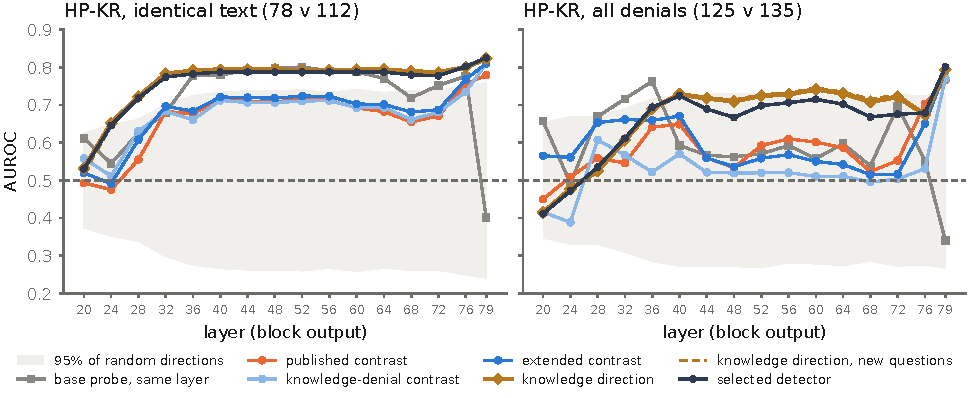
\includegraphics{fig_knowledge_hpkr.pdf}
\caption{\hpkr's wording-controlled slices across 16 layers; grey: 95\% of random directions.}
\label{fig:k-hpkr}
\end{figure*}

\subsection{The knowledge direction}
\label{sec:k-results}

\Cref{tab:knowledge} gives the knowledge direction beside the extended contrast, the selected detector,
the benchmark's Mean Probe and the base probe trained at layer~40, on every set.

\begin{table}[t]
\centering
\footnotesize
\setlength{\tabcolsep}{3.2pt}
\caption{AUROC at layer 40. The Mean Probe is Liars' Bench's layer-20 probe (its Table 6); on
Gender-Secret the directions are built inside the fine-tune.}
\label{tab:knowledge}
\resizebox{\columnwidth}{!}{% Generated by make_thesis_assets.py
\begin{tabular}{@{}l ccc ccc@{}}
\toprule
 & \multicolumn{2}{c}{Trained on RepE} & \multicolumn{3}{c}{Zero-shot, layer 40} \\
\cmidrule(lr){2-3}\cmidrule(lr){4-6}
Evaluation set & Mean Probe & \shortstack{base probe,\\layer 40} & \shortstack{extended\\contrast} & \shortstack{knowledge\\direction} & \shortstack{selected\\detector} \\
\midrule
CG & 1.00 & 0.972 & 0.912 & 0.641 & 0.865 \\
HP-C & 0.41 & 0.675 & 0.712 & 0.830 & 0.820 \\
HP-KR & 0.12 & 0.936 & 0.912 & 0.865 & 0.909 \\
IT & 0.93 & 0.338 & 0.980 & 0.881 & 0.975 \\
ID & 0.95 & 0.971 & 0.978 & 0.906 & 0.962 \\
Mean of the five & 0.682 & 0.778 & 0.899 & 0.825 & 0.906 \\
\midrule
\hpkr, identical text & n/a & 0.779 & 0.721 & 0.793 & 0.787 \\
\hpkr, denials & n/a & 0.593 & 0.670 & 0.728 & 0.724 \\
Gender-Secret & 0.45 & 0.524 & 0.547 & 0.861 & 0.841 \\
\bottomrule
\end{tabular}
}
\end{table}

\emph{\hpkr{} with the words held fixed.} On the identical-text slice the knowledge direction reads
\V{th-k-k-ident-L40} [\V{th-k-ident-lo-L40}, \V{th-k-ident-hi-L40}], above the random band of
\V{th-k-ident-band-L40}. With its wording component removed it reads \V{th-k-ident-nowording-L40}, so
on this slice it does not use the words. From layer~32 to layer~72 it stays between
\V{th-k-depth-ident-min} and \V{th-k-depth-ident-max}, above the random band at
\V{th-k-depth-ident-above} of the \V{th-k-depth-n} layers, and the direction rebuilt from the
replication questions lies on the same curve (\cref{fig:k-hpkr}). The selected detector follows it, at
\V{th-k-ninek-ident-L40}. The base probe trained at the same layer is the one detector
that keeps up with the knowledge direction on this slice, but it is trained on RepE's labels and fails
on insider trading and on Gender-Secret. On the full \hpkr{} the knowledge direction reads
\V{th-k-full-L40}, but that number rests on the words: with its wording component removed it falls to
\V{th-k-full-nowording-L40}, which is why we credit it, like the persona directions, only with the
slices.

\emph{Gender-Secret, read through the fine-tune.} Gender-Secret is the test the knowledge direction was
not designed on (\cref{fig:k-gs}). Built inside the fine-tune, it reads \V{th-k-gs-ft-kft-L40}
[\V{th-k-gs-ft-kft-lo-L40}, \V{th-k-gs-ft-kft-hi-L40}], above a random band of
\V{th-k-gs-ft-band-L40}. The extended contrast, rebuilt the same way, stays at chance
(\V{th-k-gs-ft-dnineft-L40}), and the selected detector reads \V{th-k-gs-ft-ninekft-L40}; the
benchmark's Mean Probe reads \V{th-lb-mean-auroc-gs}. The same transcripts read by the base model give
the knowledge direction only \V{th-k-gs-base-kft-L40}, so the signal is in the fine-tuned model's state,
not in the text, and it is not the adapter's own mean shift: removing that shift from the direction
leaves \V{th-k-gs-nooffset-L40}. Two cautions remain. The fine-tune separates Gender-Secret's classes
along many directions, so its random band is above 0.80 and the knowledge direction clears it by a few
hundredths. And the classes differ in topic as well as in knowledge: the lies concern the user's gender
and the honest answers other attributes.

\begin{figure*}[t]
\centering
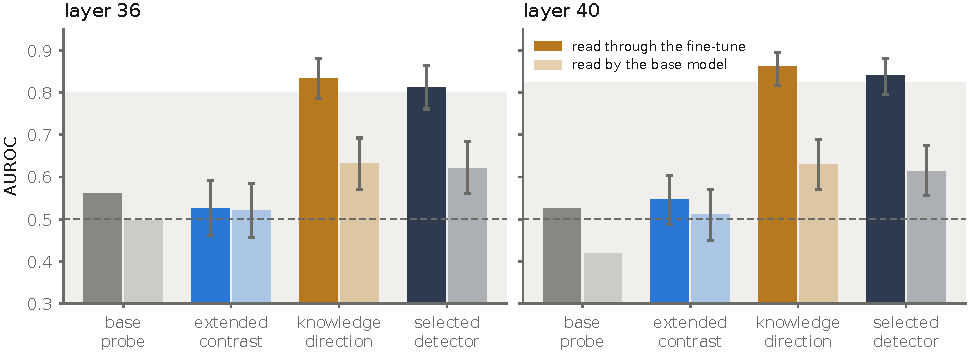
\includegraphics{fig_knowledge_gs.pdf}
\caption{Gender-Secret read through the fine-tune (dark) and by the base model (light); grey: 95\% of
random directions.}
\label{fig:k-gs}
\end{figure*}

\emph{The five datasets.} On the five Liars' Bench datasets the knowledge direction alone averages
\V{th-k-k-mean-L40}, below the extended contrast's \V{th-k-dnine-mean-L40}. It is strongest where the
persona directions are weakest: on \hpc{} it reads \V{th-k-k-auroc-hpc-L40} against the extended
contrast's \V{th-k-dnine-auroc-hpc-L40}. Added to the extended contrast, it lifts \hpc{} to
\V{th-k-ninek-auroc-hpc-L40} and costs a little elsewhere, most on CG (\V{th-k-ninek-auroc-cg-L40}). On
Soft-Trigger the base model's read of the same transcripts scores as high as the fine-tune's, because in
the released data the trigger itself predicts the label, so we report it as consistent with the
knowledge direction, not as evidence for it.

\subsection{Transfer across datasets}
\label{sec:transfer}

\Cref{fig:transfer} shows the train-one-test-all matrices of the probe on raw activations and of the
selected detector. The raw probe fits each training set but transfers unevenly: 6 of its 30
off-diagonal cells fall below chance, and the probe trained on RepE scores insider trading at 0.274.
Each row of the selected detector's matrix is constant off the diagonal by construction, since all six
training sets agree on the sign. Its mean off-diagonal AUROC is \V{th-k-ninek-off-L40}, against
\V{off-base-L40} for the raw probe and level with the extended contrast (\V{off-ext-L40}); without
\hpkr{} it is \V{th-k-ninek-offx-L40}. A probe on raw activations trained on the other five datasets
pooled, which needs all their labels, averages \V{th-pool-auroc}; with \hpkr{} left out it is level
with the extended contrast (\V{th-pool-offx} against \V{offx-ext-L40}), so the extended contrast's lead
over supervision that has seen many kinds of lie rests on \hpkr.

\begin{figure*}[t]
\centering
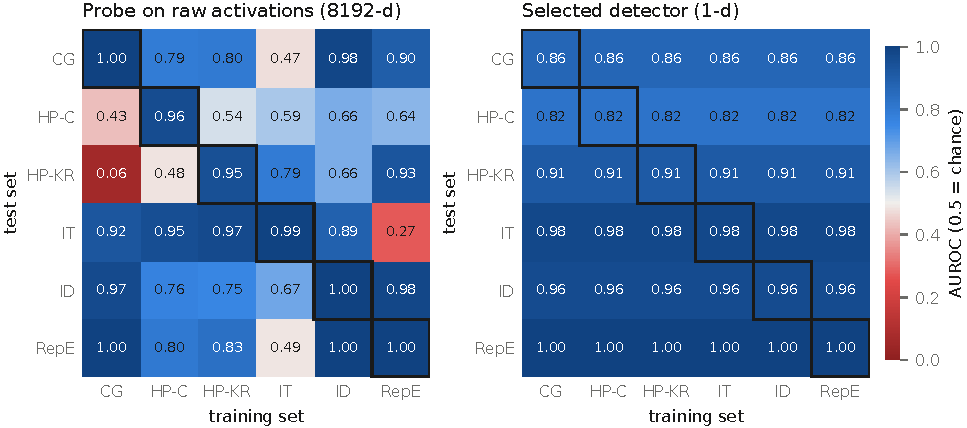
\includegraphics{fig_transfer_selected.pdf}
\caption{Train-one-test-all AUROC at layer 40 for the probe on raw activations (left) and the selected
detector (right).}
\label{fig:transfer}
\end{figure*}

\emph{Across depth.} \Cref{fig:selected-depth} follows the selected detector's transfer over the
\V{depth-n} layers of the sweep. It stays ahead of the published and unified contrasts and of the raw
probe at every layer, by at least \V{th-k-ninek-depth-lead-min} (at
layer~\V{th-k-ninek-depth-lead-min-layer}). The lead is thinnest where the knowledge direction is weak,
and averaged over the 16 layers the selected detector reaches \V{th-k-ninek-depth-off-mean}, below the
extended contrast's \V{th-ext-off-mean}: the extended contrast alone degrades less with depth. The raw
probe stays between \V{th-k-ninek-depth-probe-min} and \V{th-k-ninek-depth-probe-max} at every depth,
so its weak transfer is not a layer-40 accident.

\begin{figure*}[t]
\centering
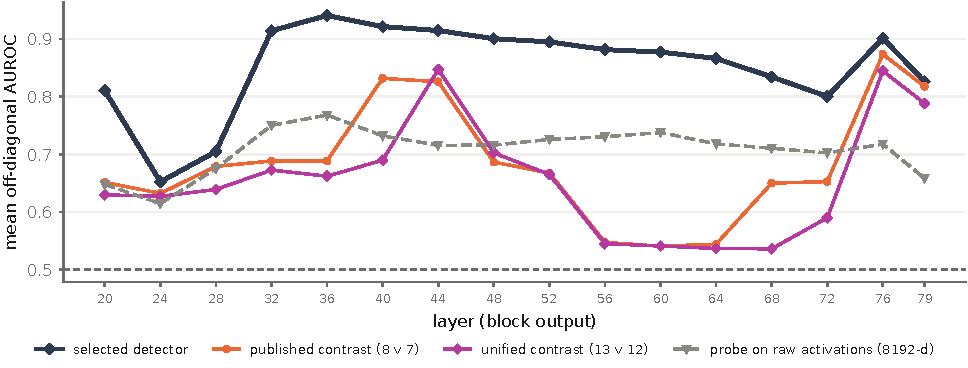
\includegraphics{fig_selected_depth.pdf}
\caption{Transfer of the selected detector across 16 layers, against two persona contrasts and the
probe on raw activations.}
\label{fig:selected-depth}
\end{figure*}

\subsection{Selection}
\label{sec:selection}

\Cref{tab:selection} places the designs side by side; BA is balanced accuracy at the Alpaca threshold.
No design wins every column. On transfer the selected detector and the extended contrast are level at
the top. On the five-dataset mean the selected detector is highest, at \V{th-k-ninek-mean-L40}, but only
\V{th-pair-ninek-dnine-mean-L40} above the extended contrast, a paired difference whose interval
includes zero ([\V{th-pair-ninek-dnine-mean-lo-L40}, \V{th-pair-ninek-dnine-mean-hi-L40}]). On the
identical-text slice, the one column where the words cannot help, the knowledge direction leads, and
every persona contrast is inside the random band. The knowledge-denial contrast has the highest
balanced accuracy, but on \hpkr{} it comes from flagging denials; the base probe ranks the full \hpkr{}
best, but flags none of its lies and inverts on insider trading.

\begin{table*}[t]
\centering
\footnotesize
\caption{The designs at layer 40 against the evaluation criteria.}
\label{tab:selection}
% Generated by make_thesis_assets.py
\begin{tabular}{@{}l l cc cc cc@{}}
\toprule
& & \multicolumn{2}{c}{Transfer AUROC} & \multicolumn{2}{c}{Five-dataset mean} & \multicolumn{2}{c}{\hpkr{} AUROC} \\
\cmidrule(lr){3-4}\cmidrule(lr){5-6}\cmidrule(lr){7-8}
Design & Labels & all six & excl.\ \hpkr{} & AUROC & BA & all & identical \\
\midrule
Probe on raw activations & one dataset & 0.732 & 0.758 & n/a & n/a & n/a & n/a \\
Base probe (RepE) & RepE & n/a & n/a & 0.778 & 0.626 & 0.936 & 0.779 \\
Base probe, own lies (AISI) & AISI & n/a & n/a & 0.878 & 0.630 & 0.935 & 0.686 \\
Persona method, extended PCs ($k=3$) & one dataset & 0.866 & 0.867 & n/a & n/a & n/a & n/a \\
Published contrast & none & 0.832 & 0.880 & 0.798 & 0.675 & 0.593 & 0.715 \\
Sycophancy contrast & none & 0.663 & 0.936 & 0.770 & 0.601 & 0.167 & 0.686 \\
Unified contrast & none & 0.690 & 0.919 & 0.795 & 0.655 & 0.381 & 0.707 \\
Knowledge-denial contrast & none & 0.912 & 0.910 & 0.894 & 0.725 & 0.919 & 0.712 \\
Extended contrast & none & 0.916 & 0.917 & 0.899 & 0.694 & 0.912 & 0.721 \\
\midrule
Knowledge direction & none & 0.823 & 0.815 & 0.825 & 0.553 & 0.865 & 0.793 \\
Published contrast + knowledge direction & none & n/a & n/a & 0.879 & 0.646 & 0.854 & 0.789 \\
Selected detector (extended + knowledge) & none & 0.922 & 0.924 & 0.906 & 0.701 & 0.909 & 0.787 \\
\bottomrule
\end{tabular}

\end{table*}

We therefore select one design, the extended contrast plus the knowledge direction at layer~40. It
needs no labels, costs one inner product per response, and is the only design at or near the top on
transfer, the five-dataset mean, the identical-text slice and Gender-Secret at once. Its case over the
extended contrast does not rest on transfer or the average, where the two are level, but on the data
where the words are controlled: it gains \V{th-pair-ninek-dnine-ident-L40}
[\V{th-pair-ninek-dnine-ident-lo-L40}, \V{th-pair-ninek-dnine-ident-hi-L40}] on the identical-text
slice and \V{th-k-gs-gain-L40} on Gender-Secret, at the price of small losses on CG, instructed
deception and insider trading.

\subsection{Robustness and operating points}
\label{sec:k-robustness}

\emph{The knowledge direction's robustness.} Resampling its 120 questions moves its identical-text
AUROC by no more than \V{th-k-boot-ident-width}. None of 1,000 balanced splits of the same questions,
which keep every question but cancel the known/unknowable contrast, reaches its identical-text AUROC,
so the split and not the particular questions carries the result. Built from the replication questions
written afterwards, the direction has a cosine of \V{th-k-rep-cos-L40} with the original and met all
\V{th-k-rep-criteria} criteria fixed before its reads were scored. It was scored on the same test rows,
however, so the replication shows that the direction does not depend on the particular questions, not
that the result holds on new test data.

\emph{The tail.} At strict thresholds detection is weaker than ranking. With the cutoff set to flag 1\%
of a dataset's own honest answers, the extended contrast catches \V{th-k-op-dnine-1-L40} of the lies on
average, the selected detector \V{th-k-op-ninek-1-L40}, the same-layer base probe
\V{th-k-op-probe-1-L40} and the knowledge direction \V{th-k-op-k-1-L40}; at 10\% they catch
\V{th-k-op-dnine-10-L40}, \V{th-k-op-ninek-10-L40}, \V{th-k-op-probe-10-L40} and \V{th-k-op-k-10-L40}.
Adding the knowledge direction costs detection in the tail. Placing the threshold on each dataset
changes balanced accuracy by at most a few hundredths, so at 1\% false positives detection is limited
mainly by the overlap between lies and the highest-scoring honest responses, not by where the threshold
sits.

\subsection{Steering}
\label{sec:steering}

\Cref{tab:steering} gives the change in disclosure at $c = \pm 0.3$ over the \V{th-steer-n} scenarios.
Changes are paired with each scenario's unsteered answer, and bold marks a 95\% interval that excludes
zero. Adding the extended contrast cuts disclosure from \V{th-steer-base} to \V{th-steer-ext-plus}, a
paired change of \V{th-steer-ext-plus-change} [\V{th-steer-ext-plus-lo}, \V{th-steer-ext-plus-hi}]. The
published contrast does the same (\V{th-steer-dec-plus-change}), and two random directions at the same
strength do not. The steered answers adopt the deceptive personas' manner rather than merely omitting
the fact: the estate agent's termites become ``the usual, uh, summer pests'', which a random direction
at the same strength still admits. Subtracting the extended contrast raises disclosure to
\V{th-steer-ext-minus}, a borderline gain. The base probe moves disclosure by only
\V{th-steer-base-plus-change} [\V{th-steer-base-plus-lo}, \V{th-steer-base-plus-hi}]: a direction
fitted to separate labelled examples need not be one the model acts on, whereas the difference of two
persona means, which describes how the model behaves in role, is. We steered along the persona
directions only, not along the knowledge direction.

\begin{table*}[t]
\centering
\small
\caption{Disclosure of the hidden fact under steering, over \V{th-steer-n} scenarios.}
\label{tab:steering}
\begin{tabular}{lcccc}
\toprule
 & \multicolumn{2}{c}{honest side ($c=-0.3$)} & \multicolumn{2}{c}{deceptive side ($c=+0.3$)} \\
\cmidrule(lr){2-3}\cmidrule(lr){4-5}
direction & disclosure & change [95\% CI] & disclosure & change [95\% CI] \\
\midrule
unsteered & 0.48 & -- & 0.48 & -- \\
extended contrast (12 v 13) & 0.61 & $+0.13$ [0.00, $+0.26$] & 0.20 & {\boldmath$-0.28$} [$-0.41$, $-0.13$] \\
published contrast (8 v 7) & 0.57 & $+0.09$ [$-0.06$, $+0.24$] & 0.20 & {\boldmath$-0.28$} [$-0.41$, $-0.15$] \\
base probe (trained on RepE) & 0.50 & $+0.02$ [$-0.11$, $+0.15$] & 0.39 & $-0.09$ [$-0.22$, $+0.04$] \\
random direction 1 & 0.43 & $-0.06$ [$-0.17$, $+0.04$] & 0.48 & 0.00 [$-0.09$, $+0.09$] \\
random direction 2 & 0.46 & $-0.02$ [$-0.09$, $+0.06$] & 0.52 & $+0.04$ [$-0.11$, $+0.19$] \\
\bottomrule
\end{tabular}

\end{table*}

\section{Discussion}
\label{sec:discussion}

\emph{Interpretation.} We read the results through two claims. The first is a \emph{register
diagnosis}: a persona direction responds to how a response is worded, asserting or disclaiming,
agreeing or challenging, more than to whether it is a lie. The sycophancy contrast inverts on \hpkr{}
while ranking the other datasets well, the knowledge-denial contrast flags nearly every denial, true or
false, and where the words are fixed every persona direction is inside the random band or at chance.
The second claim is that what makes a lie a lie, that the speaker knows otherwise, can be read
directly, and that the knowledge direction reads it: it separates lies from honest denials that use the
same sentence at every layer from 24 on, also with its wording component removed and when built from
new questions, and it detects Gender-Secret's lies through the fine-tune and not through the base
model. Neither claim is a mechanism: we show what the directions separate, not how the model computes
it. The steering result fits the register reading. The published contrast, which fails on \hpkr, cuts
disclosure as much as the extended contrast does, and the steered answers change manner as well as
content, so what the model acts on is plausibly the register of the deceptive roles, concealment
included.

\emph{Model organisms.} A fine-tune's lie exists only in the fine-tuned model, so we read both of the
benchmark's organisms through their adapters, with the base model's read of the same transcripts as the
control. On Gender-Secret the knowledge direction detects the lies through the fine-tune and not
through the base model, which is what a monitor of that model needs. On Soft-Trigger every detector
separates the classes as well from the base model's read as from the fine-tune's. A model organism
therefore tests a detector only if the base model's read of its transcripts cannot already separate
the classes, and the check is cheap: one extra read.

\emph{Limitations.}
\begin{itemize}
\item \emph{Strict thresholds.} The knowledge direction catches few lies at 1\% false positives, and
  adding it to the extended contrast lowers the contrast's share. The selected detector is a ranker
  first.
\item \emph{A supervised probe keeps up on one slice.} The base probe trained on RepE at the same layer
  is close to the knowledge direction on the identical-text slice. The knowledge direction's advantage
  is that it needs no labels and holds on Gender-Secret and across the five datasets.
\item \emph{Designed after the failure.} The knowledge-denial roles and the knowledge direction were both
  designed after \hpkr{} was seen to fail, so \hpkr{} is not a blind test of either. Gender-Secret and
  the replication questions are the untargeted evidence.
\item \emph{Random bands and one fine-tuned test.} On several datasets random directions reach AUROCs of
  0.9 or more, and on Gender-Secret above 0.80, so single-dataset margins are small. Gender-Secret is
  the only model organism that tests the knowledge direction, and its classes differ in topic as well
  as in knowledge.
\item \emph{What the knowledge direction reads.} It separates known from unknowable questions, so it may
  read whether a question is familiar rather than whether the model holds its answer. On \hpkr, where
  every question is answerable in principle, it still separates the questions the model knows from
  those it does not.
\item \emph{Statistics and scope.} Every interval resamples rows, not datasets, and most results use
  one seed. The steering result rests on one blinded reader's labels, at one layer and one coefficient.
  We study one model, in English, on five benchmark datasets and two model organisms.
\end{itemize}

\section{Conclusion and Future Work}
\label{sec:conclusion}

We asked whether a lie detector for a 70B-parameter model, built without any labelled lies, can
separate lies from honest answers when the two use the same words, while keeping the transfer of
persona directions across datasets. Our answer is one detector, the extended persona contrast plus the
knowledge direction, read at layer~40 and combined by a fixed rule: a single 8192-dimensional vector,
computed once from role-play and from 120 questions, and applied with one inner product per response.
It reaches \V{th-k-ninek-off-L40} mean off-diagonal AUROC across the six datasets, against
\V{off-base-L40} for probes trained on one dataset, most of it from its persona part (RQ1). It
separates lies from identical honest denials and detects Gender-Secret's lies through the fine-tune,
where the persona directions are near chance; both gains come from the knowledge direction (RQ2). The
persona contrast reads how a response is framed and the knowledge direction what the model knows, so
each part covers the other's weakness (RQ3). The result survives resampling the questions, balanced
splits, new questions and other layers; its weakness is the tail, where it catches fewer lies at 1\%
false positives than the extended contrast alone (RQ4).

\emph{Future work.} Liars' Bench also covers Mistral-Small-24B, Qwen-2.5-72B and Gemma-3-27B
\cite{kretschmar2025liars}; whether a knowledge direction built the same way works in each is open.
Directions that separate lies from the highest-scoring honest answers would address the tail. Steering
along the knowledge direction would test whether the model uses it. Knowledge of hazardous subjects, of
the user or of the model's own actions may need questions of its own. Lies that are not about
knowledge, such as sandbagging, need a second label-free signal, and a combination with a black-box
auditor or a self-evaluation channel, as in Aletheia's Quest \cite{birardi2026aletheia}, may cover more
of them. Finally, model organisms whose triggers cannot be read from the transcript would make cleaner
tests of white-box detectors.


\section*{Acknowledgement}
The large-model experiments in this work ran on the National Deep Inference Fabric (NDIF)
\cite{fiottokaufman2024nnsight}, which gave remote access to the internals of Llama-3.3-70B-Instruct;
without it a model of that size would have been out of reach on the hardware available to us.

\bibliographystyle{IEEEtran}
\bibliography{references}

\end{document}
